% =====================================================================
% Structure-Aware Row Scaling for Block-Structured Mixed-Integer Programs
% International Journal for Numerical Methods in Engineering (Wiley) -- NJD v5.
%
% COMPILE WITH XeLaTeX on TeX Live 2022 (the WileyNJDv5 class requires XeLaTeX;
% the template states TeX Live 2023 is unsupported). Sequence:
%   xelatex main ; bibtex main ; xelatex main ; xelatex main
% AMA = the journal reference style; Times1COL = single-column review layout.
% =====================================================================
\documentclass[AMA,Times1COL]{WileyNJDv5}

% --- Packages NOT already provided by WileyNJDv5 (which loads amsmath, amsthm,
%     amssymb, graphicx, hyperref, booktabs, multirow, threeparttable, float,
%     subfig, xcolor, url, ...). Only additive packages are loaded here. ---
\usepackage{mathtools}
\usepackage{bm}
\usepackage{xurl}   % breakable paths/URLs (\path)
% break long paths only at natural separators, not mid-token
\makeatletter\def\UrlBreaks{\do\/\do\_\do\-\do\.}\makeatother
\usepackage{threeparttable}
\usepackage{placeins}    % \FloatBarrier (class does not load it)
\usepackage{subcaption}  % subfig not active in this class mode; caption is loaded
\usepackage{siunitx}
\sisetup{
  detect-weight=true,
  detect-family=true,
  detect-mode=text,
  mode=text,
  group-digits=integer,
  group-minimum-digits=4,
  group-separator={,},
  table-number-alignment=center,
}
\usepackage{algorithm}
\usepackage{algpseudocode}
% orcidlink removed: fragile inside NJD \maketitle; ORCID given as text in \corres
\usepackage{lineno}                       % continuous line numbers for review
\usepackage{tikz}                          % conceptual overview figure (Fig. 1)
\usetikzlibrary{arrows.meta,positioning,calc}
\usepackage[nameinlink,noabbrev]{cleveref} % after the class-loaded hyperref

% Open in single-page (continuous) layout. The title page is an odd, right-hand page;
% in a two-page/"book" viewer the reader sees a blank sheet to its left, which reads as a
% phantom blank first page. This hint makes compliant viewers default to one page wide, so
% no facing blank appears. It only sets the default view; it changes no content.
\hypersetup{pdfpagelayout=OneColumn,
            colorlinks=true,      % no link boxes; sober dark-blue links instead
            linkcolor=blue!45!black,
            citecolor=blue!45!black,
            urlcolor=blue!45!black}

% --- Macros (theorem environments and caption styling are provided by the class) ---
\newcommand{\R}{\mathbb{R}}
\newcommand{\Z}{\mathbb{Z}}
\newcommand{\nnz}{\operatorname{nnz}}
\newcommand{\diag}{\operatorname{diag}}
\newcommand{\cond}{\operatorname{cond}}
\newcommand{\argmin}{\operatorname*{arg\,min}}
\newcommand{\norm}[1]{\left\lVert #1 \right\rVert}
\newcommand{\abs}[1]{\left\lvert #1 \right\rvert}
\newcommand{\methodBase}{Base}
\newcommand{\methodAug}{SA-Aug}
\newcommand{\methodMat}{SA-Mat}
\newcommand{\methodRuiz}{Ruiz}
\newcommand{\methodRuizCols}{Ruiz+Cols}
\newcommand{\sgm}{\ensuremath{\operatorname{sgm}}}
\newcommand{\PARten}{\ensuremath{\operatorname{PAR10}}}
\newcommand{\AvgGap}{\ensuremath{\overline{\gamma}_{\mathrm{cb}}}}
\newcommand{\Work}{\texttt{Work}}

% Figure helpers. Figures are external vector PDFs in figs/. The two-panel helper
% uses the subfigure environment from subcaption (loaded above), not the class's subfig.
\newcommand{\singleplotheight}{.42\textheight}
\newcommand{\pairedplotheight}{.30\textheight}
\newcommand{\safefigure}[2]{\includegraphics[width=#2,keepaspectratio]{#1}}
\newcommand{\plotfigure}[4]{%
  \begin{figure*}[!tbp]
  \centering
  \includegraphics[width=#2,height=\singleplotheight,keepaspectratio]{#1}
  \caption{#3}\label{#4}
  \end{figure*}%
}
\newcommand{\plotfiguretrim}[5][3pt 3pt 3pt 3pt]{%
  \begin{figure*}[!tbp]
  \centering
  \includegraphics[width=#3,height=\singleplotheight,trim=#1,clip,keepaspectratio]{#2}
  \caption{#4}\label{#5}
  \end{figure*}%
}
\newcommand{\twoplotfigure}[8]{%
  \begin{figure*}[!tbp]
  \centering
  \begin{subfigure}[t]{0.485\textwidth}\centering
    \includegraphics[width=\linewidth,height=\pairedplotheight,clip,keepaspectratio]{#1}
    \caption{#2}\label{#3}
  \end{subfigure}\hfill
  \begin{subfigure}[t]{0.485\textwidth}\centering
    \includegraphics[width=\linewidth,height=\pairedplotheight,clip,keepaspectratio]{#4}
    \caption{#5}\label{#6}
  \end{subfigure}
  \caption{#7}\label{#8}
  \end{figure*}%
}

\graphicspath{{figs/}}

% --- Front matter (NJD v5) ---
\articletype{Research Article}
\received{}
\revised{}
\accepted{}
% Pin the running folio so the title page is numbered 1 (the class otherwise leaves
% the start-page placeholder unset and prints "0" on the title page, which reads as a
% missing/blank first page); the journal overrides this at production.
\startpage{1}
% Suppress the editorial placeholders the class hardcodes ("Received/Revised/Accepted:
% Added at production", "DOI: xxx/xxxx", and the first-page footer with the generic
% journal URL and "Copyright Holder Name"); all of these are filled at production.
\historydates{}
\doiheadtext{}
\makeatletter
\def\oddfoot@titlepage@info{\vbox{\hsize\textwidth{\noindent\rule{\textwidth}{.5pt}\vskip-40pt {\fontsize{7}{8}\selectfont \hfill \foot@vertbar\quad {\pagenumfont\@FirstPg}}\vskip10pt }}}
\makeatother
% Compact the reference list slightly (without this, the last page carries only a
% handful of entries over an otherwise empty page). The class loads natbib, so the
% inter-item glue is natbib's \bibsep.
\AtBeginDocument{\setlength{\bibsep}{0.9pt plus 0.2pt}}

\begin{document}

\title{When Does Generator Metadata Help? A Controlled Study of Structure-Aware Row Scaling for Generated Mixed-Integer Programs}

\author[1]{Mathias Rodr\'iguez Castro}

\authormark{Rodr\'iguez Castro}
\titlemark{When Does Generator Metadata Help? Structure-Aware Row Scaling for Generated MIPs}

\address[1]{\orgdiv{Facultad de Ingenier\'ia}, \orgname{Universidad de la Rep\'ublica}, \orgaddress{\state{Montevideo}, \country{Uruguay}}}

\corres{Mathias Rodr\'iguez Castro, Facultad de Ingenier\'ia, Universidad de la Rep\'ublica, Montevideo, Uruguay. \email{mathiasr@fing.edu.uy} (ORCID: 0009-0002-7235-7677)}

\abstract[Abstract]{%
Generated mixed-integer programs (MIPs) reach solvers as flat coefficient matrices, though
their generators retain each row's role, block ownership, and coupling incidence. We ask
whether generator metadata should alter \emph{how} coupling constraints are scaled relative to
the local blocks they connect, beyond applying the same per-row kernel to every constraint. The
layer studied here applies geometric-mean row normalization in a local--block--coupling order,
preserves the MIP exactly, and verifies every returned solution against the original unscaled
constraints. We test it on three hydrothermal-dispatch classes, two commercial
solvers, and two MIPGap tolerances, against unscaled, Ruiz-kernel, solver-internal, and
role-blind full-coverage controls, together with a synthetic mechanism grid carrying a direct
spectral audit.

The result is controlled and regime-dependent. On the operational instances it is
\emph{non-identifying}: the distinctive coupling stage never activates, and the one substantial
difference between the selective rule and the role-blind full-coverage control traces to an
incomplete role map that left a block of market-shortage rows unscaled, not to the metadata. Under
equal coverage \emph{and an inactive coupling stage} the matrix-only policies coincide, as
\cref{prop:attribution} predicts and byte-for-byte confirms on the operational instances. When
heterogeneous block scales activate the block-relative treatment, however, the same-kernel policies
no longer coincide: on a controlled heterogeneous-block grid the matrix-only structure-aware rule
attains an order-of-magnitude lower spectral pseudo-condition number than a role-blind rule with
the \emph{same} kernel and coverage ($30/30$ instances, $p<10^{-8}$), demonstrating that the
mechanism can produce a material conditioning gain. The operational campaigns never enter that regime, where a per-row
local kernel computable from the flat matrix carries the whole effect. Runtime effects are of the
order of the solver's own
run-to-run variability---a five-seed replication puts the within-instance noise floor at
$12$--$18\%$ and leaves the metadata-versus-coverage contrast inside it in the fast class---and
only one of twelve contrasts clears multiplicity adjustment, none under CPLEX. Under the
pre-declared absolute criterion the augmented rule (SA-Aug) \emph{degrades} original-scale
reliability relative to Base, with failures concentrated on zero-right-hand-side balance rows,
and we report the strict reading as primary; the variant we ultimately recommend is the
matrix-only rule.

The transferable lesson outlives the method: the rule with the best numerical diagnostic is not
the fastest, so numerical improvement and solver acceleration must be measured separately.
}

\keywords{Numerical scaling, mixed-integer programming, generated formulations, block-structured optimization, engineering optimization, hydrothermal dispatch}

\maketitle

% Review builds carry continuous line numbers; set \reviewversionfalse for production.
\newif\ifreviewversion
\reviewversiontrue
\ifreviewversion\linenumbers\fi

\section*{Practitioner Points}
\begin{itemize}
  \item Model generators already know each row's role, block, and coupling incidence---metadata a
  flat matrix export discards but that costs nothing to reuse for numerical preprocessing.
  \item Metadata matters in the appropriate regime: under identical coverage and the same
  coefficient-only kernel, block-relative scaling reduced the spectral pseudo-condition number by
  one to two orders of magnitude as the block-scale heterogeneity increased.
  \item Cover every row: closing the incomplete-role-map gap makes the matrix-only structure-aware
  and role-blind exports coincide on the operational instances, because their coupling stages
  remain inactive there---so those instances do not test the value of the metadata itself.
  \item Time preprocessing separately from the solver---on fast instances the preprocessing cost,
  not the numerics, decided which rule looked faster, and the runtime gaps were of the order of
  the solver's own run-to-run variability (a five-seed replication put the noise floor at
  $12$--$18\%$).
  \item Re-verify every returned solution against the original unscaled constraints: SA-Aug
  degraded original-scale reliability relative to Base under the strict absolute criterion, and the
  recommended matrix-only rule must also remain subject to original-scale verification.
\end{itemize}


% -------------------------------------------------------------------------
\section{Introduction}
\label{sec:introduction}
% -------------------------------------------------------------------------

A model generator and a solver see different representations of the same optimization problem. The generator builds the model from components: hydro plants, thermal units, market rules, resource limits, demand balances, and discrete operating decisions. While doing so, it knows which rows are local to one component, which variables that component owns, and which constraints link several components. The solver receives the exported version: rows, columns, coefficients, bounds, and tolerances. In that exported matrix, much of the generator's structural knowledge has disappeared.

This loss matters because numerical representation affects computation. Two formulations
can describe the same feasible set and objective, yet lead a solver through different
presolve reductions, relaxation bases, cuts, incumbent searches, branching decisions, and
feasibility checks. Generic scaling routines can inspect coefficient magnitudes after
export. They usually cannot tell whether a row is a local turbine restriction, a thermal
limit, or a system-wide balance. The generator can make that distinction before export.
Mainstream modeling environments---Pyomo, JuMP, GAMS, AMPL---are exactly such generators:
they assemble the model component by component but, in their standard export paths, hand the
solver a flat matrix that no longer marks which rows are local, which variables a component
owns, or which rows couple components. Block-structured extensions of these ecosystems do
transport such structure---graph-based and block-decomposition modeling layers, and
solver-side decomposition files---but they feed it to decomposition algorithms rather than to
numerical preprocessing, which is the gap addressed here.

This is not made obsolete by solver-internal scaling. Commercial solvers already contain
sophisticated numerical preprocessing, and the experiments below leave it enabled; the
question here is complementary---whether an external layer can supply structural numerical
information before the solver sees the matrix as an anonymous list of rows and columns. A
positive answer would not replace solver scaling, but change the representation on which the
solver's pipeline starts.

The resulting question is simple: can generator-level block information guide positive row scalings that improve the solver-facing representation without changing the MIP? The question is not whether positive row scaling is valid. Multiplying a complete constraint by a strictly positive scalar preserves the feasible set. The question is whether the scaling factors should depend on information that the generator still has: local rows, component blocks, and coupling rows. In this sense, the paper treats pre-export metadata as numerical information rather than only as modeling bookkeeping.

We answer this question with a structure-aware row-scaling framework. The method scales
only whole constraints, including their right-hand sides. Hence it preserves the original
mixed-integer optimization problem. Its novelty lies in the order and source of the
scales, not in claiming that row scaling is new. The generator first scales local component
rows. It then summarizes the scale of each locally scaled block. A third stage would scale
global coupling rows with the scales of the blocks they connect; on every operational instance
tested its activation condition is never met, so that stage is exercised only on the synthetic
grid and is reported here as an extension rather than as validated machinery. Throughout the paper, this
local--block--coupling architecture is treated as a \emph{candidate} structure-aware policy
whose stages, coverage, and pipeline sensitivity are evaluated empirically, with the coupling
stage found to be operationally untested rather than refuted.

The contribution is not a new equilibration kernel---the per-row factor is a known
geometric-mean normalization, and the results show that this kernel carries most of the effect.
Generator metadata is useful only if the structural map is complete. In the modular formulation
every constraint is generated either by a local component or as a linking relation among
components, so the role map should be exhaustive: every row belongs to one local block or to the
coupling set (\cref{eq:role-disjointness}). The central question is therefore whether exhaustive
generator metadata improves the treatment of the \emph{coupling} rows, relative to a
kernel-matched, full-coverage role-blind rule that scales every row the same way.

We are deliberate about what the present campaigns can and cannot answer, because the
implementation used for them did not realize an exhaustive map: it left a block of
market-shortage constraints unscaled that the role-blind control normalized
(\cref{subsec:strategy-2}). That coverage gap, together with the fact that the distinctive
coupling stage never activates on any operational instance, makes the operational comparison
\emph{non-identifying} for the value of metadata---it varies coverage and metadata at once and
never exercises the one stage where metadata is structurally decisive. What the campaigns do
establish is cleaner and still useful: row scaling improves the solver-facing diagnostics and
can improve runtime over the unscaled base; the per-row local kernel, computable from the flat
matrix, carries essentially all of that effect on these instances; and, by
\cref{prop:attribution}, under equal coverage \emph{and} the inactive coupling stage of the
operational instances the structure-aware and role-blind matrix-only exports are provably---and
empirically---identical there, so no operational difference can be pinned on the metadata (once the
coupling stage activates, as it does on the heterogeneous-block synthetic grid, the two no longer
coincide). Concretely, the paper contributes: (i) an exhaustive-map formulation
of the row taxonomy and an attribution principle (\cref{prop:attribution}) that localizes any
metadata effect to the coupling rows and dictates the coverage-matched comparison the question
requires; (ii) an algebraically exact, auditable row-scaling layer for generated
block-structured MIPs, with the returned solutions verified on the original, unscaled
constraints; (iii) a controlled empirical study---augmented and coefficient-only role-blind
controls on all three classes under Gurobi and a fixed-basis conditioning control; and (iv) an
explicit separation of numerical improvement from computational acceleration. \Cref{fig:overview}
summarizes the proposed layer at a glance.

\begin{figure}[t]
\centering
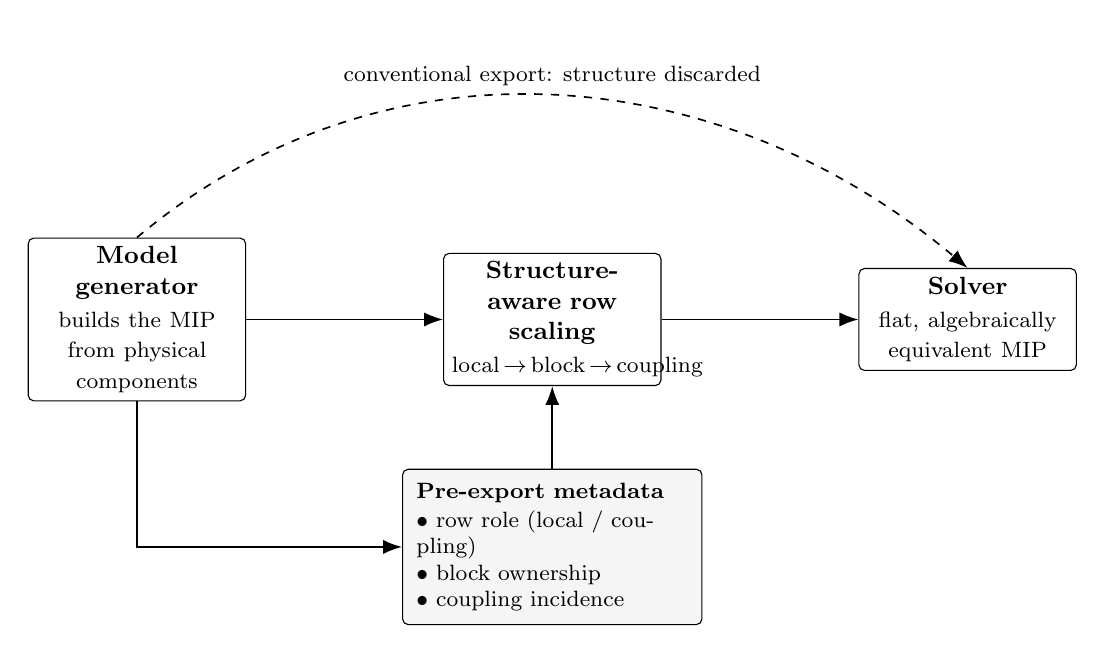
\begin{tikzpicture}[
  font=\small,
  >=Latex,
  box/.style={draw, rounded corners=2pt, align=center, minimum height=1.05cm,
              text width=2.55cm, inner sep=3pt},
  metabox/.style={draw, fill=black!4, rounded corners=2pt, align=left,
                  text width=3.45cm, inner sep=5pt, font=\footnotesize},
  arr/.style={-{Latex[length=2.4mm]}, semithick},
  darr/.style={-{Latex[length=2.4mm]}, semithick, dashed}
]
  \node[box] (gen) {\textbf{Model generator}\\[1pt]\footnotesize builds the MIP from
                    physical components};
  \node[box, right=2.5cm of gen] (scale) {\textbf{Structure-aware row scaling}\\[1pt]
                    \footnotesize local\,$\to$\,block\,$\to$\,coupling};
  \node[box, right=2.5cm of scale] (solver) {\textbf{Solver}\\[1pt]\footnotesize flat,
                    algebraically equivalent MIP};
  \node[metabox, below=1.05cm of scale] (meta) {\textbf{Pre-export metadata}\\[1pt]
                    $\bullet$ row role (local / coupling)\\
                    $\bullet$ block ownership\\
                    $\bullet$ coupling incidence};
  % main pipeline
  \draw[arr] (gen) -- (scale);
  \draw[arr] (scale) -- (solver);
  % the generator emits metadata, which keys the scaling
  \draw[arr] (gen.south) |- (meta.west);
  \draw[arr] (meta.north) -- (scale.south);
  % what a flat export throws away
  \draw[darr] (gen.north) to[out=40,in=140]
        node[above, font=\footnotesize] {conventional export: structure discarded}
        (solver.north);
\end{tikzpicture}
\caption{The proposed layer in one picture. A generator retains each row's role---local to a
component or coupling between components---block ownership, and coupling incidence before
export. A conventional export (dashed) hands the solver a flat matrix in which this structure is
lost. The structure-aware layer instead uses this metadata to assign positive row factors in a
local--block--coupling order and exports an \emph{algebraically equivalent} flat MIP. The solver
still receives a single flat matrix; only its numbers change. (The role-blind flat control, and
the coverage gap left by an incomplete role map, are analyzed in
\cref{subsec:stage-attribution}.)}
\label{fig:overview}
\end{figure}

The numerical rationale is also local--block--coupling. In an ideal block-diagonal matrix,
scalar block scaling can reduce scale separation between blocks but cannot repair a block's
intrinsic conditioning; once coupling rows are added, their relevant magnitude is their size
relative to the scaled local blocks, not their raw coefficients. Idealized conditioning
results make this reasoning precise and motivate the local--block--coupling order, but they do
not validate it and do not claim to predict mixed-integer runtime. The direct spectral audit of
\cref{subsec:spectral-audit} finds that the augmented rule obtains no conditioning advantage
over applying the same kernel to every row. By contrast, the kernel-matched heterogeneous-block
audit shows that the matrix-only block-relative rule can outperform its role-blind counterpart by
one to two orders of magnitude in spectral pseudo-conditioning: the spectral evidence is split by
rule, and it is positive for the recommended matrix-only variant.

We test the method on short-term hydrothermal dispatch, used not as a new formulation but as a
demanding testbed: it creates local hydro, thermal, market, shortage, and demand modules linked
by global balances, with coefficients mixing water volumes, turbine flows, power outputs, costs,
and penalties---block structure with strong scale heterogeneity. The intended generality,
however, is the generated block-structured MIP, not the hydrothermal equations. The layer
requires only metadata that many modular generators already have---which rows are local, which
block owns a variable or constraint, which global rows couple blocks---while reservoir dynamics,
turbine curves, and market costs determine the instances but never enter the scaling rule. The hydrothermal model thus supplies a realistic stress test for a layer whose intended target
is any generated MIP with local components and sparse global coupling. Whether the
coverage-versus-selectivity findings transfer beyond this domain, however, is not established
here: all operational results come from three instance classes of a single application, so
their generalization to other block-structured domains remains open.

The hydrothermal formulation used in the experiments descends from models for the
R\'io Negro hydroelectric complex and extensions to hydrothermal dispatch with Salto
Grande, developed by Risso and coauthors, together with a modular C++ implementation
used as the experimental platform
\cite{risso2025rioNegro,risso2025uruguayRiver,rodriguez2025thesis}.
We take the formulation as given and insert the proposed preprocessing layer after model
generation and before solver invocation.

The paper organizes its evidence into three strands of different strength: the algebraic strand
is exact (positive row scaling preserves the MIP); the numerical strand is empirical
(structure-aware scaling lowers own-incumbent path-specific fixed-LP diagnostics in the tested
instances); and the performance strand is conditional and exploratory. Under fixed-pool
intent-to-treat PAR10---an endpoint fixed after inspecting the data---some structure-aware
variant falls below Base in each Gurobi class and tolerance, though not the same variant in
each, while under CPLEX 22.1.2.0 there is no robust gain. SG-Ter-Mer at $0.1\%$ is the only cell in which both variants remain below Base
after strict reliability adjustment; this is a descriptive penalized-cost ordering, the
SA-Aug margin is negligible, and it is not replicated at $1\%$. The controlled attribution
analyses sharpen the result against the method's own premise: essentially the entire Gurobi
runtime effect is recovered by the local stage alone---a per-row geometric mean that consumes
no generator metadata---while the direct Flat comparisons make the role-based selection policy
class-, kernel-, and endpoint-dependent in the reported Gurobi campaigns. The path-specific diagnostic
moves in the intended numerical direction, but it is neither a pure measure of representation
nor a proven cause of acceleration.

The rest of the paper follows this chain of evidence. \Cref{sec:related-work} identifies
the research niche. \Cref{sec:model} defines the generated model structure and testbed.
\Cref{sec:scaling} gives the scaling method. \Cref{sec:experimental-design} explains how
the experiments test the claims. \Cref{sec:results} reports numerical and runtime
evidence. \Cref{sec:discussion} interprets that evidence and answers likely objections.
\Cref{sec:validity} states the main limitations and reproducibility implications, and
\cref{sec:conclusion} summarizes the contribution.

\section{Related work}
\label{sec:related-work}
% -------------------------------------------------------------------------

The literature sets the stage but leaves a specific niche. Hydrothermal-dispatch models provide realistic generated block-structured MIPs with heterogeneous units and global balances; numerical-scaling work explains why coefficient magnitudes matter, but its standard tools operate on the exported matrix; and formulation-quality practice shows that algebraic representation can matter as much as the underlying set. The missing argument is narrower than ``scaling is useful'': when a generator still knows each row's role and each variable's block, that metadata can be used as numerical information before export. The resulting transformation must then be evaluated separately as an algebraic equivalence, a representation change, and a performance intervention whose observed effect is specific to the tested solver pipeline.

\subsection{Hydrothermal dispatch and MIP formulations}

Hydrothermal dispatch has been studied with dynamic programming, stochastic dual
dynamic programming, nonlinear programming, and mathematical programming. Classical
references emphasize the trade-off between thermal generation costs, hydro opportunity
costs, demand satisfaction, and intertemporal reservoir management
\cite{wood2013power,conejo2010decision}. In short-term settings, MIP formulations are
attractive because they incorporate discrete decisions, piecewise-linear approximations,
local operating constraints, and system-wide balance equations in a single model
\cite{vielma2015formulation}.

This literature motivates the experimental domain but not the novelty claim. The dispatch model is used because it is a representative generated block-structured MIP: local physical modules are created separately, their variables have heterogeneous units, and a smaller set of global rows links the modules through system-wide balances. These are precisely the structural features exploited by the preprocessing layer.

\subsection{Dispatch models used in this study}

The computational experiments use a reference formulation from a research line on
MIP-based dispatch models for the Uruguayan power system. Risso et al. introduced a mixed combinatorial optimization model for the
R\'io Negro hydroelectric complex \cite{risso2025rioNegro} and extended the
modeling line to hydrothermal dispatch for the Uruguay River hydroelectric plant,
with emphasis on Salto Grande and coupled hydrothermal operation
\cite{risso2025uruguayRiver}, and an enriched formulation of the R\'io Negro model, the
closest published reference for the dispatch features used by the Full class
\cite{risso2026enriched}. The implementation used here builds on a modular
C++ version of the R\'io Negro dispatch model \cite{rodriguez2025thesis}.

This provenance fixes the scope of the experiments. The dispatch formulation, data
pipeline, and physical components are taken as given. The proposed method acts after the
model has been generated and before the solver is called. Consequently, any observed
difference between variants is attributed to an algebraically equivalent representation of
the same generated MIP, not to a modified dispatch model.

\subsection{Numerical scaling and solver-facing representation}

Scaling is a standard preprocessing operation in linear and mixed-integer optimization.
Multiplying a constraint by a positive factor preserves the feasible region but changes
the numerical magnitudes passed to the solver. These magnitudes can affect feasibility
tolerances, relaxation stability, presolve transformations, cut generation, basis quality,
and the numerical behavior of LP relaxations. Practical guidelines for difficult LP and
MIP models warn that large coefficient ranges and poor scaling can harm solver
performance even when the mathematical formulation is correct \cite{klotz2013lp,klotz2013mip},
and the dedicated treatment of identifying and correcting ill-conditioning in linear and
integer programs \cite{klotz2014illconditioning} is the closest published counterpart to the
solver-facing diagnostic apparatus this paper reports in \cref{subsec:original-scale-audit}.

This paper uses that observation in a restricted way: it does not claim coefficient compression
is itself an objective, nor that a smaller coefficient range must speed up branch-and-bound. A MIP
solver is a pipeline---presolve, internal scaling, root relaxation, cuts, heuristics, incumbents,
branching, node processing, termination---whose stages can respond differently to the same
external scaling. The experiments therefore distinguish exported coefficient-range ratios from
solver-level conditioning diagnostics and from runtime, a distinction central to interpreting the
Gurobi--CPLEX contrast.

\subsection{Generic equilibration and its limitation for generated models}

Generic equilibration procedures balance rows and columns according to matrix norms.
This is a mature subfield of numerical linear algebra. Geometric-mean and
arithmetic-mean ($\ell_\infty$) scaling normalize each row or column by an average of its
coefficient magnitudes \cite{tomlin1975scaling}; Curtis--Reid scaling chooses logarithmic
diagonal factors that minimize a least-squares measure of coefficient spread
\cite{curtisreid1972}; Sinkhorn--Knopp iteration drives a nonnegative matrix toward a
doubly stochastic form by alternating row and column normalization \cite{sinkhorn1967};
and Ruiz-type scaling iteratively equilibrates row and column norms through diagonal
transformations \cite{ruiz2001scaling}. These methods are the standard tools and are
already embedded in solver presolve and internal scaling \cite{achterberg2020presolve}.
Their computational payoff, however, is known to be irregular: the largest empirical study
of LP scaling to date found that no scaling method consistently improves---and can even
degrade---simplex performance across solvers \cite{elble2012scaling}, an early warning that
coefficient compression alone is not the lever.
Such methods are useful because they are model-agnostic and can be applied after export.
That strength is also their limitation in the setting considered here. A flat-matrix method
can see coefficient magnitudes and sparsity, but it is not told whether a row is a local
turbine restriction, a thermal bound, a market-cost relation, a shortage constraint, or a
system-wide balance.

Against this background, the proposed rule is not a new equilibration kernel: its local row
factor is, in isolation, a geometric-mean normalization of the row's nonzero coefficient
magnitudes, optionally augmented with the right-hand side (the augmented \methodAug{} kernel
includes $\lvert b_r\rvert$ among the extremes; the matrix-only \methodMat{} kernel does not). What is new is \emph{where the scales come from and in what order}---the
factors are keyed to generator metadata (row role, block ownership, coupling incidence) rather
than the flat matrix, and applied in a local--block--coupling order so coupling rows are
normalized relative to the already-scaled blocks they connect, not their raw coefficients. A flat
method (Ruiz, Curtis--Reid, geometric-mean, Sinkhorn--Knopp) cannot make this
local-versus-coupling distinction, because role information is exactly what export discards. Concretely, take two rows with
identical coefficients: a flat method cannot tell them apart and scales them identically, whereas the
structure-aware rule need not. If one is a local block row and the other a coupling row, the
local row is scaled by its own coefficients while the coupling row is scaled relative to the
\emph{already-scaled} blocks it links---so a coupling row with small raw coefficients can still
receive a large factor when it joins a poorly scaled block, and conversely. Identical numbers,
different roles, different factors: that is the distinction a flat matrix cannot expose---though, as \cref{subsec:stage-attribution} shows, this representational capability is not itself the runtime lever. The
model stays monolithic, as with generic scaling: an external, auditable layer that uses
generator metadata before the exported matrix loses it.

\subsection{Formulation quality, generated structure, and decomposition}

The MIP literature also stresses that formulation quality matters: two algebraically
related formulations can describe the same modeling intention but lead to different
relaxations, numerics, and search behavior \cite{vielma2015formulation}. On this paper's
own application class, the tight-and-compact tradition is the established answer to
whether representation changes solver behavior: reformulating the thermal unit-commitment
problem to tighten its relaxation and shrink its size yields large, repeatable solver-time
reductions \cite{carrion2006uc,moralesespana2013tight}. That strand changes the
\emph{algebraic} representation---the variables, the constraints, the feasible polytope---and
is the natural rival hypothesis to the one studied here. The present work is adjacent to it
but changes a different object. It does not strengthen the formulation, add valid
inequalities, alter variables, or change the feasible set; it changes only the positive row
multipliers applied to complete constraints. The two levers are complementary rather than
competing, and the results below---in which the numerical lever moves runtime by at most a
few percent---are consistent with the algebraic lever being the larger one on this class,
which the tight-formulation literature already documents.

The method is also adjacent to structural decomposition. Like Dantzig--Wolfe, Benders, or
Lagrangian approaches, it recognizes local blocks and global linking rows. Unlike those
methods, it does not decompose the optimization problem, introduce a master problem, or
exchange prices or cuts between subproblems. The solver still receives one monolithic MIP.
The use of block structure is numerical rather than algorithmic decomposition: block
metadata guide the representation presented to the solver.

\subsection{Remaining niche}

The resulting contribution is deliberately narrow: it tests whether local rows, block scales, and
coupling rows should be treated as different numerical objects before a generated block-structured MIP
is exported. The performance comparison rests on distributional evidence over heterogeneous
instances rather than a single runtime average, using performance profiles
\cite{dolan2002performance}, paired tests, deterministic-effort metrics, and solver-level
conditioning diagnostics.

\section{Materials and methods: generated modular formulation and testbed}
\label{sec:model}
% -------------------------------------------------------------------------

We now define the objects that the scaling rule changes and the objects it must leave
unchanged. The generator supplies the block structure; the preprocessing layer changes the
row magnitudes; the solver then receives an algebraically equivalent MIP. The dispatch
model itself is not new. What matters here is the structure that the generator exposes and
the original scale in which all feasibility and objective checks are evaluated after the
solve. We consider generated modular MIP instances formulated as
\begin{equation}
\begin{aligned}
  \min_{x} \quad & c^\top x \\
  \text{s.t.} \quad & Ax \le b, \\
  & x_j \in \Z, \qquad j \in \mathcal{I}, \\
  & x_j \in \R, \qquad j \notin \mathcal{I}.
\end{aligned}
\label{eq:generic-mip}
\end{equation}
In the general generated setting, the vector $x$ collects all variables created by the
modules, while $A$ and $b$ contain both local component constraints and global linking
constraints. In the hydrothermal testbed used here, $x$ includes generation, reservoir,
flow, spillage, shortage, and operating variables. Equalities are represented either
explicitly or by pairs of inequalities, depending on the solver interface.

The notation is intentionally application-agnostic: the layer uses the generator's structural
map---row role, block ownership, coupling incidence---not hydrological, thermal, or economic
semantics. The hydrothermal variables above explain the physical origin of the coefficients;
they are not assumptions of the scaling method.

\subsection{Hydrothermal dispatch testbed and scope}

The computational testbed uses the reference model generated by the modular dispatch
platform developed around R\'io Negro and Salto Grande hydrothermal dispatch models
\cite{risso2025rioNegro,risso2025uruguayRiver,rodriguez2025thesis}.
The application is useful because it exhibits the target structure: local modules
with heterogeneous physical units and global rows that couple those modules through
system-wide balances. The hydraulic, thermal, and market-cost constraints are those of
the reference model and its implementation.

A caveat about those heterogeneous units is in order, because it is tempting to read the
imbalance as artificial. Unit heterogeneity (reservoir volumes in $\mathrm{hm}^3$, flows in
$\mathrm{m}^3/\mathrm{s}$, power in MW) lives on the \emph{columns}, and rescaling units is,
mathematically, column scaling: an exact reformulation for continuous variables, whereas
arbitrary continuous column scaling does not in general preserve the standard integer
lattice unless the variable domains are transformed consistently, so a straightforward unit
normalization of a MIP is in practice partial. Our column-normalizing baseline
(\methodRuizCols{})
is the weakest variant in runtime, and the base is no ill-scaled straw man: it already
runs under the solver's own internal equilibration (\cref{subsec:internal-scaling}). In the
tested configurations, the row-based variants were therefore more effective than the
particular column-inclusive baseline considered here; whether a better-designed column or
unit normalization could compete is untested, and the row-only
scoping decision is revisited as a limitation in \cref{sec:validity}.

The method acts on the generated algebraic model, not the physical dispatch formulation: every transformation must preserve the feasible set and let objective values, constraint violations, and operational variables be read in the original scale after solution. It never uses a hydro-specific rule (reservoir priority, turbine efficiency, unit commitment) to choose factors---those details generate the rows, and only their structural role in the block-coupled MIP is used afterward.

\subsection{Block structure}

The method targets models generated by components or agents. Each component
$i\in\mathcal{B}$ creates local variables $x_i$, contributes local constraints
$A_i x_i\le b_i$, and appears in a smaller number of global constraints. Let
$\mathcal{R}_i$ denote the local row index set of component $i$. In the hydrothermal
testbed, these components include hydro, thermal, market, and demand modules. If $u_{\mathrm{loc}}$ stacks all local variables and $g$ denotes an aggregate
coupling variable, the row structure can be written schematically as
\begin{equation}
\begin{bmatrix}
D & 0 \\
0 & I_T \\
L & -I_T
\end{bmatrix}
\begin{bmatrix}
u_{\mathrm{loc}} \\
g
\end{bmatrix}
\sim
\begin{bmatrix}
b \\
d \\
0
\end{bmatrix},
\qquad
D=\diag(A_1,\ldots,A_B).
\label{eq:compact-dispatch-structure}
\end{equation}
Here $\sim$ denotes a row-wise relation that is $\le$, $=$ or $\ge$ depending on the block,
since the local and coupling rows mix inequalities and equalities; the scaling layer treats
all three identically, so the specific sense of each row is immaterial to what follows.
The first block contains local component restrictions. The second block represents an
aggregate system restriction. The third block contains coupling equations that link local
component decisions with the aggregate system variable. In the dispatch application,
these rows correspond to demand and balance relationships. More generally, absorbing the
aggregate variable and its defining rows into the coupling block, the coefficient matrix
takes the block form
\begin{equation}
A =
\begin{bmatrix}
A_1 & 0   & \cdots & 0 \\
0   & A_2 & \cdots & 0 \\
\vdots & \vdots & \ddots & \vdots \\
0   & 0   & \cdots & A_B \\
L_1 & L_2 & \cdots & L_B
\end{bmatrix},
\qquad
b =
\begin{bmatrix}
b_1\\ b_2\\ \vdots\\ b_B\\ h
\end{bmatrix}.
\label{eq:block-matrix}
\end{equation}
The matrices $A_i$ encode local restrictions. The matrices $L_i$ encode each block's contribution to the global coupling rows, such as demand balance in the hydrothermal
testbed.

Row roles and block incidence are separate metadata fields. Because every constraint in the
modular formulation is generated either by a single local component or as a linking relation
among components, the row-role map should be \emph{exhaustive}: each row belongs to exactly one
local block or to the coupling set. Formally, a role map
\begin{equation}
\tau:\mathcal{R}_{\mathrm{all}}\longrightarrow\mathcal{B}\cup\{\mathrm{cpl}\},
\qquad
\mathcal{R}_{\mathrm{all}}
=\Bigl(\dot{\textstyle\bigcup}_{i\in\mathcal{B}}\mathcal{R}_i\Bigr)
\,\dot\cup\,\mathcal{R}_{\mathrm{cpl}},
\qquad
\mathcal{R}_i\cap\mathcal{R}_j=\varnothing\ (i\neq j),
\label{eq:role-disjointness}
\end{equation}
sends $\tau(r)=i$ when $r$ is local to block $i$ and $\tau(r)=\mathrm{cpl}$ when it links
several blocks through the variables it involves; a coupling row is not a local row of any
block and does not enter the local-row normalization stage. We accordingly define the target
class as generated modular MIPs \emph{equipped with an exhaustive role map}, rather than assuming
that every conceivable modular MIP admits such a partition without further modeling decisions.
Within this class there is no third row category: a row that looks ``global but not coupling''
has simply not been traced to the module that generates it, so a residual class is a symptom of
an incomplete map $\tau$, not a structural fact of the formulation.

We flag this because the implementation used for the operational campaigns did \emph{not}
realize an exhaustive map. One set of rows---the market shortage segments of the SG-Ter-Mer
testbed, some $1800$ constraints---was left outside both the local blocks and the coupling
set, even though each is generated by the market/shortage module and carries that module's
variables, so each should have been assigned to that module's block. The structure-aware
rules therefore left those rows unscaled, whereas the role-blind Flat control in
\cref{subsec:stage-attribution} normalized them. That comparison consequently varies two
things at once---the use of role metadata \emph{and} the set of rows that receive any scaling
at all---so on its own it cannot attribute a difference to the metadata. We make the confound
precise, and give the attribution principle that removes it, in
\cref{prop:attribution}; we return to it when interpreting the SG-Ter-Mer result.

This structure suggests three scaling decisions: scale local rows inside each block; compute representative block scales after local row scaling; and scale global coupling rows with those block scales. The goal is to reduce harmful scale heterogeneity without erasing the modular meaning of the formulation.

\subsection{Algebraic equivalence and spectral diagnostics}
\label{subsec:equivalence-diagnostics}

We restrict the preprocessing layer to positive row scalings. This restriction makes the
transformation auditable: variables keep their original units, and the generated MIP remains
the same optimization problem. Let $D_r=\diag(d_1,\ldots,d_m)$, with $d_r>0$ for every
row. We replace $(A,b)$ by
\begin{equation}
\widetilde A = D_r A,
\qquad
\widetilde b = D_r b .
\label{eq:row-scaling}
\end{equation}
For every vector $x$,
\begin{equation}
Ax\le b
\quad\Longleftrightarrow\quad
D_rAx\le D_rb,
\label{eq:row-scaling-equivalence}
\end{equation}
because each component of the inequality is multiplied by a strictly positive scalar.
Thus positive row scaling preserves the feasible set, the integer restrictions, and the
objective function. Any difference observed after preprocessing must therefore come from
the numerical representation seen by the solver, not from a different mathematical MIP.

The theoretical arguments below use the spectral condition number as a diagnostic of linear-algebraic sensitivity. For a real matrix $M$, define
\begin{equation}
\kappa_2(M)=
\frac{\sigma_{\max}(M)}{\sigma_{\min}^{+}(M)},
\label{eq:spectral-condition}
\end{equation}
where $\sigma_{\max}(M)$ is the largest singular value and $\sigma_{\min}^{+}(M)$ is the
smallest positive singular value. For rectangular matrices, this ratio is used only as a
diagnostic over the nonzero singular spectrum; in the square benchmarks below the minimum
is taken over the full spectrum, so that singularity is reported as an infinite condition
number. This diagnostic does not characterize the full difficulty of a MIP. A MIP solver also depends on presolve, cuts, branching, primal heuristics, incumbent discovery, feasibility tolerances, and integrality. The role of $\kappa_2$ is narrower still: it provides an idealized matrix argument for why
local rows and coupling rows \emph{might} warrant different treatment. Whether role differentiation
improves conditioning is an empirical question, and the spectral audit gives a split answer. Every
scaling rule improves $\kappa_2$ by orders of magnitude; the augmented collective rule obtains no
advantage over its role-blind counterpart on the original mechanism grid, whereas the
kernel-matched heterogeneous-block experiment shows a clear advantage for the matrix-only
block-relative rule under identical coverage (\cref{subsec:spectral-audit}).

\subsection{Ideal block scaling}
\label{subsec:ideal-block-scaling}

The block structure is not only a modeling convenience. It identifies what scalar scaling
can and cannot repair. In a purely block-diagonal matrix $D=\diag(A_1,\ldots,A_B)$, a
single scalar per block can remove differences of scale between blocks, but it cannot
improve the intrinsic conditioning of an individual block. The following benchmark makes
this statement precise in the ideal square nonsingular case.

\begin{proposition}[Ideal scalar scaling of block-diagonal matrices]
\label{prop:ideal-block-scaling}
Let $D=\diag(A_1,\ldots,A_B)$, where every $A_i$ is square and nonsingular. Let
$M_i=\sigma_{\max}(A_i)$ and $m_i=\sigma_{\min}(A_i)>0$. Then
\begin{equation}
\min_{\alpha_i>0}
\kappa_2\!\left(\diag(\alpha_1 I,\ldots,\alpha_B I)D\right)
=
\max_i \kappa_2(A_i).
\label{eq:ideal-block-minimax}
\end{equation}
One minimizer is
\begin{equation}
\alpha_i=\frac{1}{\sqrt{M_i m_i}}
=
\frac{1}{\sqrt{\sigma_{\max}(A_i)\sigma_{\min}(A_i)}} .
\label{eq:ideal-block-factor}
\end{equation}
\end{proposition}

\noindent The proof, which constructs the optimal scalar per block and evaluates the
resulting spectrum, is given in the Supporting Information (Section~S1).

This proposition is not used as an algorithmic recipe: the generated MIPs here contain
rectangular local matrices, inequalities, bounds, redundant rows, and integer variables, so
singular-value-based block scalings would not be a practical external preprocessing rule. It
instead justifies the architecture---poor scale separation between blocks should be treated
differently from poor conditioning inside a block, and after local row scaling each block
should contribute a representative scale before coupling rows are processed---and the
implemented rules replace the ideal quantities $(M_i,m_i)$ with cheap coefficient-based
proxies. As stated at the outset of this section, these are design principles, not performance
theorems. \Cref{subsec:spectral-audit} tests them and finds support for the block-relative
placement of the matrix-only kernel in heterogeneous-block regimes, but not for the augmented
collective coupling rescale.

\subsection{Effect of global coupling rows}
\label{subsec:global-coupling-theory}

Local block scaling does not exhaust the numerical issue because the generated model is
not purely block diagonal. In the hydrothermal dispatch testbed, global rows couple local
agent decisions through demand and balance equations. The relevant schematic block is
\begin{equation}
A_{\mathrm{bal}}=
\begin{bmatrix}
D & 0\\
L & -I_T
\end{bmatrix},
\label{eq:balance-block-matrix}
\end{equation}
where $D=\diag(A_1,\ldots,A_B)$ represents the local blocks and $L$ collects the
coefficients by which local decisions enter the global balance. If $D$ is nonsingular, then
\begin{equation}
A_{\mathrm{bal}}=
\begin{bmatrix}
I & 0\\
LD^{-1} & -I_T
\end{bmatrix}
\begin{bmatrix}
D & 0\\
0 & I_T
\end{bmatrix}.
\label{eq:balance-factorization}
\end{equation}
This factorization separates local scale from coupling scale. The matrix $L$ by itself is
not the relevant object: the coupling felt by the balance row after the local block scales
are taken into account is $LD^{-1}$. Thus a row with moderate entries in $L$ can still be
numerically influential if some local block contains weak directions.

The next result makes the dependence on the effective coupling norm explicit.

\begin{proposition}[Conditioning of a triangular coupling factor]
\label{prop:triangular-coupling}
Let $R\in\R^{m\times n}$ and define
\begin{equation}
T_R=
\begin{bmatrix}
I_n & 0\\
R & I_m
\end{bmatrix}.
\end{equation}
If $\rho=\norm{R}_2$, then
\begin{equation}
\kappa_2(T_R)=
\frac{\rho^2+2+\rho\sqrt{\rho^2+4}}{2}
=
\left(\frac{\sqrt{\rho^2+4}+\rho}{2}\right)^{\!2} .
\label{eq:link-condition}
\end{equation}
The sign of the identity block is immaterial: since
$\bigl[\begin{smallmatrix}I&0\\R&-I\end{smallmatrix}\bigr]
=\diag(I,-I)\bigl[\begin{smallmatrix}I&0\\-R&I\end{smallmatrix}\bigr]$ and orthogonal
factors preserve singular values, the same formula applies to the factor with $-I_T$ in
\cref{eq:balance-factorization}.
\end{proposition}

\noindent The proof, which bounds the effect of the coupling factor on the extreme
singular values, is given in the Supporting Information (Section~S1).

Applied to \eqref{eq:balance-factorization}, the proposition shows that the balance row
should not be treated as an ordinary local row. Its numerical effect depends on the
effective coupling proxy $\norm{LD^{-1}}_2$, not only on the raw magnitude of the
entries in $L$. Moreover, if a common positive factor $\gamma$ is applied to the coupling
row, the scaled block satisfies
\begin{equation}
\begin{bmatrix}
D & 0\\
\gamma L & -\gamma I_T
\end{bmatrix}
=
\begin{bmatrix}
I & 0\\
\gamma LD^{-1} & -I_T
\end{bmatrix}
\begin{bmatrix}
D & 0\\
0 & \gamma I_T
\end{bmatrix}.
\label{eq:scaled-balance-factorization}
\end{equation}
Thus $\gamma$ changes both the effective coupling term and the relative scale of the
aggregate variable in the balance equation: pushing $\gamma$ down improves the triangular
factor of \cref{eq:scaled-balance-factorization} but degrades its diagonal factor, and
vice versa. This is the trade-off behind the proposed coupling treatment---global rows
are scaled after local rows, using block-level representative scales, rather than by an
isolated row norm---and the augmented rule resolves it explicitly by minimizing the
product of the two factors (\cref{eq:augmented-coupling-factor} in
\cref{subsec:strategy-1}). In the implemented variants, $D^{-1}$ and singular values are
replaced by coefficient-based block proxies, yielding a cheap operational approximation
to the ideal coupling measure.

The same factorization yields the attribution principle that governs the experimental design.

\begin{proposition}[Attribution under an exhaustive row map]
\label{prop:attribution}
Suppose the role map $\tau$ of \eqref{eq:role-disjointness} is exhaustive, and that the
structure-aware and role-blind policies apply the \emph{same} per-row kernel to every local
row. Then both policies produce identical scaled local blocks, so any difference between the two
exported matrices is confined to the coupling rows $\mathcal{R}_{\mathrm{cpl}}$ and is
attributable exclusively to the block-relative coupling treatment. In particular, if every
coupling-candidate factor equals one or is rejected by the safeguards, the two exported matrices
are identical.
\end{proposition}

\noindent The argument is immediate. Under an exhaustive $\tau$ the two policies scale exactly
the same rows; on a local row the structure-aware rule reduces to the shared per-row kernel, so
the two agree row by row off $\mathcal{R}_{\mathrm{cpl}}$; and on a coupling row the only
structural degree of freedom is the block-relative factor $\gamma$ of
\eqref{eq:scaled-balance-factorization}, which the flat rule instead reads from the raw
coefficients. \Cref{prop:attribution} is the lever the experiments need. It says exactly where
generator metadata \emph{can} matter---the coupling rows---and therefore why the local stage
alone, computable from the flat matrix, cannot demonstrate the metadata's value; it tells us how
to read the activation audit, since a run with no coupling activation lands in the
``every factor equals one'' case where the two exports must coincide; and it fixes the valid
comparison: to measure the worth of the metadata, the structure-aware and role-blind rules must
be run under a common, exhaustive coverage, so that the two exports differ, if at all, only on
the coupling treatment. A comparison in which one rule leaves rows unscaled that the other
normalizes measures coverage, not metadata.


\subsection{From ideal diagnostics to implementable proxies}
\label{subsec:ideal-to-proxies}

The two propositions identify \emph{which} numerical distinctions a scaling rule can
preserve in the ideal square, nonsingular setting, and they motivate rather than validate
the architecture that follows. They suggest three design
requirements: local scale imbalance should be reduced before global coupling rows are
diagnosed; blocks should be summarized only after their local rows are on a comparable
scale; and a coupling row should be scaled relative to the blocks it connects, not only
relative to its own raw coefficient norm. The implemented method encodes these
distinctions through coefficient-based proxies: they are cheap to compute from the
generated model before export, auditable because they depend only on visible row and
block metadata, and they avoid expensive or unstable singular-value information from the
rectangular, redundant, inequality-based matrices that arise in generated MIPs. The row
factor based on the geometric mean of the smallest and largest nonzero magnitudes is a
robust coefficient-scale proxy that centers each eligible row without changing variables,
bounds, integrality, or the objective. Encoding a distinction is not the same as exercising
it: on the operational classes only the first stage, local row centring, ever alters the
exported matrix, because the coupling proxy stays below its activation threshold throughout
(\cref{subsec:stage-attribution}).

The coupling rule implements the same logic. In \cref{prop:triangular-coupling}, the
relevant ideal object is the effective coupling magnitude after local scaling, a term of
the form $LD^{-1}$; since generated blocks are rectangular, possibly redundant, and not
inverted by the preprocessing layer, the block scale $s_i$ used below is a representative
coefficient scale for block $i$ computed after local row scaling, and the coupling proxy
divides each coupling coefficient by the representative scale of the block owning its
column. This is a cheap, auditable surrogate for asking whether the coupling row is large
relative to the local numerical scale of the blocks it links.

We state the scope of this argument once and plainly: the propositions describe square,
nonsingular blocks under exact SVD scaling, the proxies act on rectangular,
inequality-based matrices, and we establish no bound relating the proxy scale to the
ideal spectral factor in \cref{prop:ideal-block-scaling}. The propositions motivate the
architecture; whether the architecture moves the quantity they describe is an empirical
question, and the synthetic matrices are small enough to answer it directly by singular-value
decomposition rather than through the magnitude-range surrogate the implementation uses.
\Cref{subsec:spectral-audit} reports that audit. Its verdict is split, and we state both
halves here because they bear on different claims. The propositions' \emph{qualitative}
prediction survives: every scaling rule reduces $\kappa_2$ by orders of magnitude wherever
row-multiplicative imbalance is present. Their use as a rationale for the \emph{augmented
collective} coupling factor does not: the role-blind control matches or beats the augmented
structure-aware rule on $\kappa_2$ in every pattern, including the coupling patterns the coupling
stage was designed for. The block metadata itself is not inert, though: a kernel-matched test
(\cref{subsec:spectral-audit}) isolates an order-of-magnitude $\kappa_2^{+}$ gain for the
matrix-only structure-aware rule over its role-blind control once the blocks sit at heterogeneous
scales. The spectral argument therefore supports scaling in general, and the block-relative
placement of the per-row kernel specifically, but not the augmented collective coupling rescale.

This design rationale also explains why the proposed method is row-based. Positive row scaling
preserves the original units and domains of all variables; integer and binary variables do
not require reinterpretation, and objective coefficients are left in their original
economic units. Column scaling can be useful as a generic numerical device, so a
Ruiz-plus-column baseline is included in the experiments. It is not part of the proposed
structure-aware layer because that layer is the object under study: a row-based,
algebraically transparent transformation whose row-role and coupling metadata is precisely
what the controlled comparison against role-blind coverage is designed to evaluate.


% -------------------------------------------------------------------------
\section{Numerical scaling method}
\label{sec:scaling}
% -------------------------------------------------------------------------

The scaling method keeps the same structural roles visible throughout: local rows, blocks, and coupling rows. Local rows receive row factors first. Blocks then inherit representative scales from their scaled local rows. Coupling rows receive their factors last, using the blocks they connect. This order is the algorithmic expression of the numerical argument in \cref{subsec:ideal-block-scaling,subsec:global-coupling-theory} and of the proxy interpretation in \cref{subsec:ideal-to-proxies}.

This section defines the numerical transformations tested in the results. The base variant is the unscaled model generated by the platform. The two proposed variants share the local--block--coupling architecture but are \emph{two different structural rules}: they differ both in whether the right-hand side participates in the scale diagnosis and in how coupling rows are treated (a single grid-selected factor in \methodAug{}, one factor per row in \methodMat{}), so their head-to-head comparison is not by itself a clean right-hand-side ablation. The clean ablation of the right-hand side is the local-only pair of \cref{subsec:stage-attribution}, whose members differ \emph{only} in whether $b$ enters the per-row extremes. The comparison with the Ruiz-kernel baselines tests the choice of per-row kernel under the same structural pipeline; the fully role-blind comparisons are carried by kernel-matched Flat-Aug and Flat-Mat controls (\cref{subsec:added-controls,subsec:stage-attribution}).

\subsection{Base formulation}

The \methodBase{} variant is passed to the solver without external scaling. Internal
solver presolve and internal scaling remain enabled unless stated otherwise. All
speedups, objective deviations, and original-scale reliability checks are computed relative
to this variant on the same instance, solver, and gap setting (algebraic equivalence itself
is proved analytically and needs no per-instance check).

\subsection{Augmented structure-aware scaling}
\label{subsec:strategy-1}

The first proposed variant, denoted \methodAug{}, computes row factors from both
coefficient magnitudes and right-hand sides. The motivation is that a generated row may
have moderate coefficients but a right-hand side in a very different physical or economic
scale. Such a row can still lead to a poorly balanced numerical representation.

For each local row $r$, define
\begin{equation}
\mathcal{S}_r^{A,b}
=
\left\{
\abs{a_{rj}}: a_{rj}\neq 0
\right\}
\cup
\left\{
\abs{b_r}: b_r\neq 0
\right\}.
\label{eq:augmented-set}
\end{equation}
If $\mathcal{S}_r^{A,b}\neq\emptyset$, let
\begin{equation}
M_r^{A,b}=\max \mathcal{S}_r^{A,b},
\qquad
m_r^{A,b}=\min \mathcal{S}_r^{A,b}.
\label{eq:augmented-extremes}
\end{equation}
The local row factor is
\begin{equation}
\alpha_r^{A,b}=\frac{1}{\sqrt{M_r^{A,b}m_r^{A,b}}}.
\label{eq:alpha-augmented}
\end{equation}
The scaled row is
\begin{equation}
\alpha_r^{A,b}a_r^\top x\le \alpha_r^{A,b}b_r.
\end{equation}

The rule is a three-stage procedure: rescale local rows, summarize the resulting block scales
(a diagnosis---the scales are never applied to the blocks, only to the coupling proxy), and scale
coupling rows against those block scales. On the operational classes the third stage is inert
(\cref{subsec:stage-attribution} records zero activations), so the solver there receives a
row-by-row normalization of the role-selected local rows; the coupling stage activates only on the
oversized synthetic patterns of \cref{subsec:synthetic-results}.
After local scaling, let $\widetilde a_{rj}=d_r\,a_{rj}$ for local rows, where $d_r$ is the
factor \emph{actually applied}---$d_r=\alpha_r^{A,b}$ when the candidate factor
$\alpha_r^{A,b}=1/\sqrt{M_r^{A,b}m_r^{A,b}}$ passes the safeguards of
\cref{subsec:safeguards} and $d_r=1$ when it is rejected---so the extremes below are taken
on the matrix that is actually exported, not on candidate factors. For each
local block $i$, define
\begin{equation}
M_i^{A,b}
=
\max_{r\in\mathcal{R}_i,\,j:\,\widetilde a_{rj}\neq 0}
\abs{\widetilde a_{rj}},
\qquad
m_i^{A,b}
=
\min_{r\in\mathcal{R}_i,\,j:\,\widetilde a_{rj}\neq 0}
\abs{\widetilde a_{rj}}.
\label{eq:augmented-block-extremes}
\end{equation}
The representative scale of block $i$ is
\begin{equation}
s_i^{A,b}=\sqrt{M_i^{A,b}m_i^{A,b}}.
\label{eq:augmented-block-scale}
\end{equation}
For a coupling row $r$, let $\beta(j)$ denote the local block that owns column $j$.
Columns owned by no block enter at the arithmetic mean of the valid block scales,
\begin{equation}
s_{\mathrm{free}}=\frac{1}{\lvert\mathcal{B}_+\rvert}\sum_{i\in\mathcal{B}_+}s_i^{A,b},
\qquad
\mathcal{B}_+=\{i:0<s_i^{A,b}<\infty\},
\label{eq:free-column-scale}
\end{equation}
falling back to $s_{\mathrm{free}}=1$ if no block has a valid scale, and components that
contribute no local rows enter at unit scale. The effective coupling proxy of row $r$ is
\begin{equation}
\widehat\rho_r^{A,b}
=
\sqrt{
\sum_j
\left(
\frac{\abs{a_{rj}}}{s_{\beta(j)}^{A,b}}
\right)^2
},
\label{eq:augmented-coupling-rho}
\end{equation}
the magnitude of the row relative to the representative scales of the blocks it connects,
and $\rho=\max_r \widehat\rho_r^{A,b}$ is the worst such magnitude over the coupling
rows. \methodAug{} then computes a \emph{single candidate} factor
$\gamma^{A,b}$ for the coupling block, chosen to minimize the conditioning
surrogate that the idealized analysis suggests, and applies it to each coupling row that
passes the per-row safeguards of \cref{subsec:safeguards}:
\begin{equation}
\gamma^{A,b}=\argmin_{\gamma}\,\Phi(\gamma),
\qquad
\Phi(\gamma)=\kappa_T(\gamma\rho)\,\kappa_B(\gamma),
\qquad
\kappa_B(\gamma)=\frac{\max(\bar M,\gamma)}{\min(\bar m,\gamma)},
\label{eq:augmented-coupling-factor}
\end{equation}
where $\kappa_T(\cdot)$ is exactly $\kappa_2$ of the triangular coupling factor
(\cref{eq:link-condition}), $\kappa_B$ is the diagonal spread once the aggregate variable
enters at scale $\gamma$, and, writing $\kappa_i=M_i^{A,b}/m_i^{A,b}$ for the
post-local-normalization coefficient spread of block $i$,
\begin{equation}
\bar M=\max_i\sqrt{\kappa_i},\qquad \bar m=\min_i\tfrac{1}{\sqrt{\kappa_i}}.
\label{eq:augmented-diagonal-spread}
\end{equation}
Here $\kappa_i=M_i^{A,b}/m_i^{A,b}$ is block $i$'s post-normalization coefficient spread, and
$\bar M,\bar m$ are the extrema each block would present under a \emph{virtual} normalization by
$s_i^{A,b}$ that enters only the diagonal surrogate---the blocks themselves are never scaled.
Minimizing $\Phi$ over a fixed logarithmic grid ($121$ points in $[10^{-6},10^{6}]$) resolves the
trade-off of \cref{eq:scaled-balance-factorization}: a smaller $\gamma$ improves the triangular
coupling factor and worsens the diagonal one, and by submultiplicativity $\Phi$ bounds the
ideal-scale $\kappa_2$ of the balance block; on the exported rectangular matrices it is only a
coefficient-proxy surrogate, with no formal bound claimed (\cref{subsec:ideal-to-proxies}). The
stage is skipped when the coupling is moderate ($\rho\le 10$, a per-instance test that holds
throughout the operational classes) or when $\gamma^{A,b}$ lies in the near-identity band
$(0.5,2)$; surviving coupling rows are subject to the per-row safeguards of
\cref{subsec:safeguards}, so the exported map has entries in $\{1,\gamma^{A,b}\}$ and, since
$\rho=\max_r\widehat\rho_r$ may be set by a row the floor later vetoes, $\gamma^{A,b}$ is a
single-pass candidate rather than the minimizer for the final matrix.

\subsection{Matrix-only structure-aware scaling}
\label{subsec:strategy-2}

The second proposed variant, denoted \methodMat{}, uses the same row--block--coupling
architecture but excludes $b$ from the diagnosis. The right-hand side is still multiplied
by the selected row factor to preserve equivalence, but it does not influence factor
selection. This variant is the one we ultimately recommend: excluding the right-hand side
makes the kernel structurally safe against residual amplification (\cref{subsec:safeguards}) and
gives it the best-conditioned behaviour in the spectral audit (\cref{subsec:spectral-audit}),
whereas the augmented rule of the previous subsection is better read as an exploratory probe of
whether the right-hand side should enter the diagnosis at all---a question the reliability
evidence (\cref{subsec:original-scale-audit}) answers in the negative, since folding $\lvert
b_r\rvert$ into the extremes is exactly what degrades original-scale reliability on
right-hand-side-dominated rows.

For each local row $r$, define the nonzero coefficient extremes
\begin{equation}
M_r^{A}=\max_{j:\,a_{rj}\neq 0}\abs{a_{rj}},
\qquad
m_r^{A}=\min_{j:\,a_{rj}\neq 0}\abs{a_{rj}}.
\label{eq:matrix-row-extremes}
\end{equation}
If the row has at least one nonzero coefficient, the row factor is
\begin{equation}
\alpha_r^{A}=\frac{1}{\sqrt{M_r^{A}m_r^{A}}}.
\label{eq:matrix-row-factor}
\end{equation}
The scaled row is
\begin{equation}
\alpha_r^{A}a_r^\top x\le \alpha_r^{A}b_r.
\end{equation}
This factor centers the smallest and largest nonzero coefficient magnitudes of the row
around a common scale. Unlike Euclidean-norm scaling, it does not directly depend on
the number of nonzeros in the row.

Let $\widetilde a_{rj}=d_r a_{rj}$ after local row scaling, where $d_r=\alpha_r^A$ when the
candidate factor passes the safeguards of \cref{subsec:safeguards} and $d_r=1$ otherwise,
so the block extremes below are taken on the matrix actually exported, as in \methodAug{}.
For each local block
$i$, define
\begin{equation}
M_i^{A}
=
\max_{r\in\mathcal{R}_i,\,j:\,\widetilde a_{rj}\neq 0}
\abs{\widetilde a_{rj}},
\qquad
m_i^{A}
=
\min_{r\in\mathcal{R}_i,\,j:\,\widetilde a_{rj}\neq 0}
\abs{\widetilde a_{rj}}.
\label{eq:matrix-block-extremes}
\end{equation}
The representative block scale is
\begin{equation}
s_i^A=\sqrt{M_i^A m_i^A}.
\label{eq:matrix-block-scale}
\end{equation}
No additional multiplier is applied to all rows or columns of block $i$ at this stage.
The quantity $s_i^A$ is an auxiliary representative scale: it is used only to
normalize the contribution of block $i$ when the coupling-row proxy is computed.

For a coupling row $r$, with the same ownership map $\beta(\cdot)$ and the same
convention for blockless columns as in \cref{subsec:strategy-1}, define
\begin{equation}
\widehat{\rho}_r^{A}
=
\sqrt{
\sum_j
\left(
\frac{\abs{a_{rj}}}{s_{\beta(j)}^{A}}
\right)^2
}.
\label{eq:matrix-coupling-rho}
\end{equation}
If $\widehat{\rho}_r^{A}>0$, the coupling-row factor is per row,
\begin{equation}
\gamma_r^{A}=\frac{1}{\widehat{\rho}_r^{A}},
\label{eq:matrix-coupling-factor}
\end{equation}
clipped to $[10^{-8},10^{8}]$ and subject to the safeguards below. When the block
extremes of \cref{eq:matrix-block-extremes} are computed, the implementation restricts
them to coefficients inside a fixed moderation window $(10^{-6},10^{6})$, so a single
extreme coefficient cannot distort $s_i^A$. If no post-local-scaling coefficient of block
$i$ falls inside that window, block $i$ contributes no representative scale and its columns
enter the coupling proxy at the matrix-only mean block scale
\begin{equation}
s_{\mathrm{free}}^{A}=\frac{1}{\lvert\mathcal{B}_A^{+}\rvert}\sum_{i\in\mathcal{B}_A^{+}}s_i^{A},
\qquad
\mathcal{B}_A^{+}=\{i:0<s_i^{A}<\infty\},
\label{eq:free-column-scale-mat}
\end{equation}
with $s_{\mathrm{free}}^{A}=1$ when $\mathcal{B}_A^{+}=\varnothing$; this is the
matrix-only counterpart of \cref{eq:free-column-scale}, computed from $s_i^A$ rather than
$s_i^{A,b}$.

\methodAug{} and \methodMat{} therefore differ in \emph{two} respects: whether $b$
participates in factor selection, and the granularity and criterion of the coupling
treatment (one grid-selected $\gamma$ for the whole coupling block versus one
$\gamma_r$ per row). A difference between them cannot be attributed to the right-hand
side alone; the clean right-hand-side ablation is the local-only pair reported with the
coupling-stage activation audit (\cref{subsec:stage-attribution}), which shares every other
design choice.

\subsection{Safeguards}
\label{subsec:safeguards}

All applied scaling factors---the local row factors and the coupling-row factors in the
augmented or matrix-only variants---are subject to the near-identity and
admissible-coefficient-range safeguards, applied
independently to each factor. The collective \methodAug{} coupling factor is additionally
subject to the reliability floor defined at the end of this subsection, and the optional
local reliability floor of that same paragraph applies to the augmented local factors.
The representative block scales $s_i$ are auxiliary
quantities used to compute coupling-row proxies; they are not applied as independent
row or column scalings.

\paragraph{Near-identity threshold}
A factor is applied only if it departs from one by at least a factor of $u=2$; factors
falling in the open band $(1/u,\,u)=(0.5,\,2)$ are treated as negligible and skipped:
\begin{equation}
\theta \text{ is applied}
\iff
\left(\theta \le \frac{1}{u}\right)\ \text{or}\ \left(\theta \ge u\right),
\qquad u=2 .
\label{eq:near-identity}
\end{equation}
This prevents re-scaling rows or coupling rows that are already at a reasonable scale.

\paragraph{Admissible coefficient range}
A factor is applied only if it keeps every affected coefficient within the window
$[\varepsilon_{\min},\varepsilon_{\max}] = [10^{-9},\,10^{9}]$. Writing
$c_{\min}$ and $c_{\max}$ for the smallest and largest magnitudes of the affected
coefficients, the factor $\theta$ is admitted only if
\begin{equation}
\begin{aligned}
\varepsilon_{\min} &\le c_{\min}\,\theta,
& c_{\max}\,\theta &\le \varepsilon_{\max},\\
[\varepsilon_{\min},\varepsilon_{\max}]&=[10^{-9},\,10^{9}].
\end{aligned}
\label{eq:coef-window}
\end{equation}
Otherwise, the factor is not applied and the corresponding row or coupling row is left at its base scale. The coupling factor is additionally hard-clipped to
$\gamma \in [10^{-8},\,10^{8}]$ prior to this check.

\paragraph{Reliability safeguards}
The coefficient window bounds the magnitudes of the scaled coefficients, but it does not
by itself bound the effect of a small total row factor $d_r$ on the \emph{original-scale}
residual. The exported row is $d_r$ times the original, so \emph{if} the returned point
satisfies the exported row to absolute residual at most $\varepsilon$, the corresponding
original-scale residual is at most $\varepsilon/d_r$; a small $d_r$ amplifies it. This is a
conditional relation, not a solver-level guarantee: commercial solvers enforce feasibility on
internally scaled and presolved representations, so a small $\varepsilon$ on the exported row
is expected rather than certified, and the floors below control the potential amplification
from $d_r$ rather than certify the residual. The \emph{coefficient-only} per-row kernel is
structurally safe against this amplification for its coefficients: its factor
$\alpha_r=1/\sqrt{M_r m_r}$ maps the largest coefficient to $\alpha_r M_r=\sqrt{M_r/m_r}\ge1$,
so the largest scaled coefficient is at least one (this centers the extremes geometrically
around one; it does \emph{not} preserve the original magnitude---for $M_r/m_r=10^{12}$ a
leading coefficient of $10^{12}$ becomes $10^{3}$), and consequently, under a fixed residual
bound on the exported row, the original residual relative to the row's leading coefficient
is not amplified above that bound. The \emph{augmented} kernel does not share this property:
because $\lvert b_r\rvert$ enters the extremes, a row whose right-hand side dominates its
coefficients receives a tiny $d_r$, and this is visibly the source of the largest absolute
entries in the operational audit, which sit on rows of very large right-hand side
(\cref{subsec:original-scale-audit}). Two reliability safeguards are considered: the
collective coupling floor, enabled by default, and an optional local floor evaluated
separately.

The \emph{collective coupling floor} guards the single \methodAug{} coupling factor, which
is chosen to fit the largest coupling rows and has no per-row protection: $\gamma$ is applied
to a coupling row only if the row's largest scaled coefficient magnitude remains at least
$\varepsilon_{\mathrm{floor}}^{\mathrm{cpl}}=10^{-3}$; rows below it keep their base scale.
This is enabled by default, and it eliminates the
common-factor failure mode on the synthetic suite (\cref{subsec:synthetic-results}). The
optional \emph{local floor} defines a variant we call \methodAug{}-LF, which guards the
augmented local factors directly: the local factor is applied only if it also satisfies
\begin{equation}
\alpha_r^{A,b}\ge\varepsilon_{\mathrm{floor}}^{\mathrm{loc}}
\qquad(\text{in addition to \cref{eq:near-identity,eq:coef-window}}),
\label{eq:local-floor}
\end{equation}
so that $d_r\ge\varepsilon_{\mathrm{floor}}^{\mathrm{loc}}$ bounds the conditional original
residual by $\varepsilon/\varepsilon_{\mathrm{floor}}^{\mathrm{loc}}$; a factor below the
floor leaves the row at base scale. \methodAug{}-LF is off by default and is evaluated
separately at $\varepsilon_{\mathrm{floor}}^{\mathrm{loc}}=10^{-2}$. Because the condition
on $\alpha_r$ is not invariant to a positive re-emission of a row, it is keyed to the
generator's canonical physical-unit export---the reference used by the original-scale
audit; that caveat, invariant alternatives, and the sensitivity sweep are in Table~S4.
Neither floor is a general guarantee, and the primary \methodAug{} results deliberately
retain the unresolved local-reliability behavior rather than masking it.

Because each admitted factor is a strictly positive multiplier applied to a complete
constraint---both its coefficients and its right-hand side---the feasible set and the
objective value are preserved exactly. The safeguards therefore restrict only the
numerical aggressiveness of the transformation, never its equivalence to the base model.

\paragraph{Verification protocol}
Algebraic equivalence concerns the mathematical program; it does not by itself guarantee
that the solution the solver returns for the scaled formulation satisfies the original
constraints within a given absolute tolerance. Every experiment therefore follows a fixed
protocol: (i) solve the scaled formulation; (ii) evaluate the returned solution on the
original, unscaled model (mapping variables back to original units only where column
scaling is used); (iii) check the absolute residuals of every row, bound, and
integrality restriction against the thresholds of \cref{subsec:metrics}---the formal
pass/fail criterion is absolute; right-hand-side-normalized residuals
(\cref{eq:relative-residual}) are reported descriptively when interpreting exceedances; and (iv) treat a
failed check as a numerical-reliability event---in an operational deployment such a run
would be repeated with more conservative solver settings or fall back to the base
formulation. \Cref{subsec:original-scale-audit} reports this verification for all
campaigns.

\subsection{Ruiz-type baselines}

We compare the proposed variants with two \emph{kernel-swap} baselines that run inside the
same structural pipeline. The first,
\methodRuiz{}, replaces the local per-row kernel with iterative max-norm equilibration
applied to the block row sets; the
second, \methodRuizCols{}, adds continuous-column
scaling and physical normalization. Both retain the row classification and the shared
coupling stage (which never activates on the operational classes, where
$\widehat\rho\le10$ throughout, but does act on the synthetic benchmark;
\cref{subsec:synthetic-results}). They are therefore \emph{not} fully role-blind
flat-matrix methods: they isolate the choice of \emph{kernel} under the same selection
policy, while the fully role-blind selection controls---each kernel with no roles at
all---are Flat-Aug and Flat-Mat in \cref{subsec:stage-attribution}.

\methodRuiz{} is deliberately not a weak foil: max-norm equilibration is a standard, strong
scheme, and \methodRuizCols{} additionally grants it the column-scaling lever the
structure-aware rule forgoes. Together with the Flat controls these baselines separate two
questions---whether the geometric-mean kernel differs from a Ruiz kernel
under the same selection policy, and whether role-based selection differs from full
coverage under the same kernel; the separate ``could the solver have done
this itself'' control is the internal-scaling baseline of \cref{subsec:internal-scaling}. Every
variant hands the solver the same monolithic MIP; only the pre-export row factors differ.

The final implementation uses
\begin{equation}
K=4
\end{equation}
Ruiz iterations. Binary and integer variables are not rescaled unless explicitly stated,
so that bounds, objective interpretation, and integrality remain unchanged.

\subsection{Algorithmic summary}

The recommended exhaustive matrix-only rule is collected end to end as Algorithm~S1 in the
Supporting Information; the augmented exploratory variant differs from it in two independent ways---it
folds the right-hand side into the per-row and per-block magnitude extremes, and it replaces the
per-row coupling factors with a single collective factor.

The matrix-only algorithm follows the same local and block stages with the
coefficient-only set $\{\abs{a_{rj}}:a_{rj}\neq 0\}$ and the representative block scales
and coupling proxies of \cref{eq:matrix-block-scale,eq:matrix-coupling-rho}; its coupling
stage differs in granularity, assigning each coupling row its own factor
$\gamma_r^{A}=1/\widehat\rho_r^{A}$ (\cref{eq:matrix-coupling-factor}) instead of the
single grid-selected $\gamma^{A,b}$. \methodMat{} is therefore a second structural rule,
not a right-hand-side ablation of \methodAug{}: the two differ both in whether $b$ enters
the diagnosis and in the coupling criterion, and only their local-only reductions
(\cref{subsec:stage-attribution}) isolate the right-hand side cleanly.

% -------------------------------------------------------------------------
\section{Experimental design}
\label{sec:experimental-design}
% -------------------------------------------------------------------------

\subsection{Instance classes and scenarios}

The experiments are organized around five reader questions: does scaling preserve the original
optimization problem, does it change the numerical representation, does that change solver
behavior, does any observed change depend on using generator metadata rather than applying the
same kernel to all rows, and does the answer differ across instance class, solver, and
tolerance? The fourth question is the one this study turns on. It is carried by the role-blind
Flat controls of \cref{subsec:added-controls,subsec:stage-attribution} rather than by the
contrast with the unscaled base; those controls were run under Gurobi only, so the cross-solver
persistence of their ordering remains untested. The study uses
three instance classes generated by the same modular hydrothermal platform, built from
operational instances with available real input data. The pools are balanced by construction:
every variant is attempted on every instance of a class (204 Simple, 68 SG-Ter-Mer, 34 Full).
Valid-run counts nevertheless differ slightly across class--scenario--variant cells because
individual runs can time out, abort, or lack a required diagnostic. Descriptive metrics use all
valid runs for a row (so a cell may report, say, $195$--$199$ of $204$ Simple instances).
Speedups and paired tests use scenario-specific matched base--variant pairs. One-sided timeouts
or algorithmic aborts are retained at the capped time, as defined in the statistical-analysis
subsection; pairs are excluded only when both sides fail to complete or when the instance is
uniformly unavailable for the documented infrastructure and artifact-curation reasons reported
in Supporting Information.

Each measurement is tied to the part of the argument it can support: algebraic equivalence
is proved analytically, and the numerical reliability of each returned solution is checked
by the original-scale feasibility and integrality tests (with variables mapped back to
original units only for the column-scaling baseline); the numerical
claim by exported coefficient-range summaries and solver-level conditioning diagnostics; the
performance claim by matched base--variant speedups, deterministic effort, performance
profiles, and primal--dual progress, which show that an external scaling pass changes solver
behavior but cannot attribute that change to the metadata selectivity; whether the selectivity
is responsible at all by the direct kernel-matched role-blind contrasts (\methodAug{} versus
Flat-Aug and \methodMat{} versus Flat-Mat) and the stage and coupling-activation audits of
\cref{subsec:added-controls,subsec:stage-attribution}; and the sensitivity of the observed
preprocessing effect to the tested solver pipeline through separate Gurobi and CPLEX scenarios
at two tolerances.

\begin{table*}[t]
\centering
\caption{Three instance classes test the method on progressively different generated hydrothermal models.}
\label{tab:instance-stats}
\begin{threeparttable}
\small
\begin{tabular}{@{}p{0.16\textwidth}p{0.42\textwidth}p{0.28\textwidth}r@{}}
\toprule
Class & Configuration & Main role & Instances \\
\midrule
Simple & R\'io Negro + fixed demand + fixed dispatch & Basic numerical behavior & 204 \\
Full & R\'io Negro nonlinear + Salto Grande + thermal units + market & Largest integrated model & 34 \\
SG-Ter-Mer & Salto Grande + thermal units + market & Coupled hydrothermal subset & 68 \\
\bottomrule
\end{tabular}
\begin{tablenotes}[flushleft]\footnotesize
\item The counts report the maximum operational instance pools with available real input
      data. Scenario tables may show different $n$ values because each aggregate row uses
      the valid runs available for that solver--gap--variant combination. Pairwise
      speedups and tests use matched base--variant pairs only.
\end{tablenotes}
\end{threeparttable}
\end{table*}

\noindent \Cref{tab:instance-stats} separates the three pools: Simple gives the largest
sample for distributional evidence, Full is the smallest and most integrated model, and
SG-Ter-Mer isolates a coupled hydrothermal subset---so the averages and paired tests do not come
from a single homogeneous population.

The class names are application-specific, but the three classes differ structurally---from a
simpler modular model to larger and more strongly coupled ones---so they probe whether the rule
behaves consistently across that range. All three, however, are hydrothermal-dispatch classes
produced by one generator on one platform, so the conclusions here are empirical statements
about these instances. Whether the same behavior carries over to other block-structured
engineering MIPs is a hypothesis this evidence motivates but does not test.


We evaluate four solver--gap scenarios. The operational time limit is uniformly
$T_{\max}=3600$\,s (one hour) per solve; the separate synthetic mechanism check uses $600$\,s.
Internal solver presolve and internal scaling are left enabled, because the goal is
to test whether external preprocessing helps in a realistic solver pipeline. All main
experiments were run on ClusterUY, a collaborative high-performance computing
platform for scientific computing in Uruguay \cite{nesmachnow2019clusteruy}.

\begin{table*}[t]
\centering
\caption{Four solver--tolerance scenarios examine how the observed external-preprocessing effect changes across solver pipelines and MIPGap tolerances.}
\label{tab:solver-scenarios}
\begin{threeparttable}
\small
\begin{tabular}{@{}clc@{}}
\toprule
Scenario & Solver & Relative MIPGap \\
\midrule
1 & Gurobi & $10^{-2}$ \\
2 & Gurobi & $10^{-3}$ \\
3 & CPLEX  & $10^{-2}$ \\
4 & CPLEX  & $10^{-3}$ \\
\bottomrule
\end{tabular}
\begin{tablenotes}[flushleft]\footnotesize
\item Deterministic time is reported when available: \Work{} units for Gurobi and ticks
for CPLEX.
\end{tablenotes}
\end{threeparttable}
\end{table*}

\noindent The four scenarios in \cref{tab:solver-scenarios} vary two dimensions separately: the stopping tolerance and the solver pipeline. Scenarios 1--2 test Gurobi at two MIPGap values; scenarios 3--4 repeat the comparison under CPLEX and serve as a solver contrast.



\noindent The configuration in Table~S20 matters because the proposed preprocessing is tested on top of each solver's default numerical pipeline. The CPLEX conclusions below are therefore statements about this version and ClusterUY environment, not claims about all CPLEX releases or parameter choices.



\FloatBarrier
\subsection{Controlled synthetic block-structured benchmark}
\label{subsec:synthetic-benchmark}

The hydrothermal testbed evaluates the proposed preprocessing rule on realistic
operational generated MIPs. To complement this real-data setting, we define a controlled
synthetic benchmark whose purpose is diagnostic rather than physical. The synthetic
instances are not intended to model a power system. They isolate the numerical mechanism
targeted by the method by allowing local-row scale imbalance and coupling-row scale
imbalance to be varied independently.

Each synthetic instance consists of $B$ local blocks. Block $i$ contains continuous
activity variables $y_i\in\R^{n_y}_+$ and binary activation variables
$z_i\in\{0,1\}^{n_z}$. A nonnegative slack vector $s$ is added to the global coupling
constraints to guarantee feasibility. The generic synthetic MIP is
\begin{equation}
\begin{aligned}
\min_{y,z,s}\quad
& \sum_{i=1}^{B} c_i^\top y_i
  + \sum_{i=1}^{B} q_i^\top z_i
  + P\mathbf{1}^\top s \\
\text{s.t.}\quad
& R_i y_i + G_i z_i \le r_i,
  \qquad i=1,\ldots,B,\\
& 0 \le y_{ik} \le U_{ik}z_{ik},
  \qquad i=1,\ldots,B,\quad k=1,\ldots,n_y,\\
& \sum_{i=1}^{B} L_i y_i
  + \sum_{i=1}^{B} H_i z_i
  + s \ge d,\\
& s\ge 0,\qquad z_i\in\{0,1\}^{n_z}.
\end{aligned}
\label{eq:synthetic-mip}
\end{equation}
The first group of constraints defines local block restrictions, the second group links
continuous activity variables to binary activation variables, and the third group creates
global coupling rows. The penalty $P$ is chosen large enough that the slack variable is
used only when the activated block capacity cannot satisfy the synthetic demand.

The unscaled coefficients are generated from bounded random distributions with controlled
sparsity. Local matrices $R_i$ and $G_i$ define block-internal resource constraints.
Coupling matrices $L_i$ and $H_i$ define the contribution of each block to the global rows.
The generator records row metadata
\begin{equation}
\texttt{row\_type}\in\{\texttt{local},\texttt{coupling}\},
\qquad
\texttt{block\_id}\in\{1,\ldots,B\},
\label{eq:synthetic-row-metadata}
\end{equation}
and column metadata identifying the block associated with each variable. This metadata is
the same information required by the structure-aware scaling rules.

Scale imbalance is introduced after the clean synthetic MIP has been generated. For each
eligible row $r$, a positive row multiplier
\begin{equation}
\theta_r = 10^{\xi_r},
\qquad
\xi_r\sim\mathcal{U}[-S,S],
\label{eq:synthetic-row-factor}
\end{equation}
is drawn and applied to the entire row, including its right-hand side. Therefore, the
scaled representation is algebraically equivalent to the clean synthetic MIP. The severity
parameter $S$ controls the possible scale range. We use
\begin{equation}
S\in\{0,3,6\},
\label{eq:synthetic-severity}
\end{equation}
corresponding to no artificial imbalance, moderate imbalance, and strong imbalance.

Five scale patterns are considered:
\begin{enumerate}
  \item \textbf{None:} no artificial row scaling is applied.
  \item \textbf{Local:} only local block rows are multiplied by factors
  \eqref{eq:synthetic-row-factor}.
  \item \textbf{Coupling:} only global coupling rows are multiplied by factors
  \eqref{eq:synthetic-row-factor}, one independent draw per row---heterogeneous
  imbalance \emph{among} the coupling rows.
  \item \textbf{Coupling-uniform:} all global coupling rows are multiplied by a
  \emph{single} shared factor $\theta=10^{\xi}$, $\xi\sim\mathcal{U}[-S,S]$, one draw per
  instance---a collective, units-mismatch-style displacement of the coupling rows relative
  to the blocks, which is the case the block-relative coupling stage is designed for.
  \item \textbf{Mixed:} both local block rows and global coupling rows are multiplied,
  independently per row.
\end{enumerate}
The ``none'' pattern is a negative control: a useful preprocessing rule should not create
large artificial changes when the representation is already reasonably scaled. The
``local'' and two coupling patterns isolate the numerical objects distinguished by the
proposed method, and the two coupling patterns separate the collective displacement a
single block-relative factor can repair from the per-row heterogeneity it cannot. The
``mixed'' pattern approximates the combined heterogeneity observed in
generated models. These controlled patterns are mechanism checks. They verify that the implementation reacts correctly when the source of imbalance is known by construction, but they are not an operational local-only versus coupling-only ablation on the real hydrothermal instances.
In the generated instances the local and coupling row sets are disjoint, as in the method's
row taxonomy (\cref{sec:scaling}): a coupling row is incident to several blocks through its
variables, but it is not a local row of any of them and does not enter the local-row
normalization stage.


\begin{table*}[t]
\centering
\caption{Controlled synthetic benchmark factors isolate the numerical mechanisms targeted by the scaling rule.}
\label{tab:synthetic-design}
\begin{threeparttable}
\small
\begin{tabular}{@{}p{0.18\textwidth}p{0.20\textwidth}p{0.26\textwidth}p{0.27\textwidth}@{}}
\toprule
Factor & Levels used & Controlled object & Purpose \\
\midrule
Scale pattern & none, local, coupling, coupling-uniform, mixed
& Row class affected by artificial scaling
& Separate local imbalance from per-row and collective coupling imbalance \\
Severity $S$ & $0,3,6$
& Range of row multipliers $10^{-S}$--$10^S$
& Test mild and severe numerical heterogeneity \\
Blocks and size & $B=10$, $n_y=n_z=8$
& Number and size of generated local components
& Keep a fixed block structure while varying row-scale imbalance \\
Rows and seeds & $8$ local rows per block, $3$ coupling rows, $20$ seeds
& Random coefficients and sparsity patterns
& Estimate distributional behavior rather than one instance \\
\bottomrule
\end{tabular}
\begin{tablenotes}[flushleft]\footnotesize
\item The synthetic instances are not physical power-system models. They are controlled
block-structured MIPs designed to test whether the preprocessing rule responds to the type
of scale imbalance it is designed to exploit. The reported synthetic grid uses the middle
size $B=10$, the five patterns, the three severity levels, and twenty random seeds per
pattern--severity cell.
\end{tablenotes}
\end{threeparttable}
\end{table*}

The reported synthetic runs follow the factor grid summarized in \cref{tab:synthetic-design},
using the five scaling variants in \cref{subsec:variants} plus the role-blind flat control
introduced in \cref{subsec:stage-attribution}, the
same original-scale feasibility and objective checks, Gurobi with relative MIPGap
$10^{-3}$, and a $600$ second time limit. They are intentionally small: the benchmark is a
controlled mechanism check for global magnitude-range behavior and original-scale numerical
reliability, not a performance experiment. Runtime claims are reserved for the operational
hydrothermal instances. The legacy CSV fields \texttt{kappa\_antes}/\texttt{kappa\_despues}
store the augmented global magnitude-range proxy
\begin{equation}
\mathcal M(A,b)=
\{\,|a_{rj}|:a_{rj}\ne0\,\}\cup\{\,|b_r|:b_r\ne0\,\},
\qquad
\widehat\kappa_{\mathrm{range}}(A,b)=
\frac{\max\mathcal M(A,b)}{\min\mathcal M(A,b)},
\label{eq:synthetic-range-proxy}
\end{equation}
not the spectral condition number $\kappa_2(A)$. The synthetic tables, figures, and tests
below use \cref{eq:synthetic-range-proxy}, which is the quantity the implementation itself
optimizes. Because these matrices are small, we additionally compute $\kappa_2(A)$ exactly
for the whole grid and compare the two; \cref{subsec:spectral-audit} reports that comparison.

\subsection{Scaling variants}
\label{subsec:variants}

The compared variants are: \methodBase{}, the original formulation; \methodAug{},
the augmented structure-aware scaling rule; \methodMat{}, the matrix-only
structure-aware rule with safeguards; \methodRuiz{}, a Ruiz-kernel baseline that swaps
the local geometric-mean kernel for max-norm row equilibration ($K=4$ iterations) inside
the same structural pipeline; and \methodRuizCols{}, the same with
continuous-column scaling and physical normalization. Both Ruiz variants keep the row
taxonomy and the shared coupling stage and are therefore \emph{not} fully role-blind; the
fully role-blind operational baselines are Flat-Aug and Flat-Mat in
\cref{subsec:stage-attribution} (the synthetic grid uses Flat-Aug).
Binary and integer variables are not rescaled.

\subsection{Additional controls: internal scaling, sensitivity, and coupling-stage activation}
\label{subsec:added-controls}

Three further controls sharpen the attribution of the main comparison. They reuse the same
matched-pairs design, the same instance classes, and the same original-scale verification,
and they leave the five variants above unchanged.

\paragraph{Solver-internal-scaling baseline}
To separate ``structure-aware external scaling helps'' from ``any extra scaling pass
helps, and the solver could have produced it,'' we run the \emph{unscaled} model under the
solver's own scaling controls and compare it, within each scenario, against the
structure-aware variants run under default internal scaling. For Gurobi we sweep the scaling
flag over its admissible settings (no scaling, equilibration, geometric, and aggressive
modes); for CPLEX we sweep its read-scaling parameter (none, default equilibration,
aggressive). If a tuned internal setting matches the structure-aware runtime on the same instances, whatever
runtime change is observed reduces to generic coefficient compression the solver could have
produced itself; if it does not, the change requires an external pass. This control bears only
on whether the pass must be external, not on whether generator metadata is needed to construct
it: that question is settled by the role-blind Flat contrasts of
\cref{subsec:stage-attribution}.
Presolve remains enabled throughout. Internal scaling is varied only in this control's
solver-specific sweep (including the setting that disables it), while the structure-aware
variants always run under the solver's default internal-scaling configuration, as in the
main experiments.

\paragraph{Hyperparameter sensitivity}
The constants of the proposed rules are, for \methodAug{}: the near-identity band $u=2$
(\cref{eq:near-identity}), the admissible coefficient window
$[\varepsilon_{\min},\varepsilon_{\max}]=[10^{-9},10^{9}]$ (\cref{eq:coef-window}), the
coupling activation threshold $\widehat\rho>10$, the collective coupling reliability floor
$\varepsilon_{\mathrm{floor}}^{\mathrm{cpl}}=10^{-3}$, the
$\gamma$ grid ($121$ log-uniform points on $[10^{-6},10^{6}]$), and the hard clip
$[10^{-8},10^{8}]$; the optional \methodAug{}-LF variant adds the local floor
$\varepsilon_{\mathrm{floor}}^{\mathrm{loc}}=10^{-2}$ (off by default). \methodMat{} shares
$u$, the window, and the clip, and adds the
moderation window $(10^{-6},10^{6})$ on the block extremes. The Ruiz iteration count $K=4$
is a parameter of the baselines, not of the proposed rules. Three sensitivity analyses are
reported; each varies one constant at a time within a single cell, so together they bound
knife-edge sensitivity to individual constants rather than validate the safeguard cascade as a
deployable policy. On the Simple class under Gurobi at the $1\%$ tolerance we sweep
$u\in\{1.5,2,4\}$ and the coefficient window over
$\{[10^{-6},10^{6}],[10^{-9},10^{9}],[10^{-12},10^{12}]\}$: within that cell the runtime
conclusion is unchanged ($\sgm$ within $[2.01,2.12]$\,s across the sweep, against
$3.73$\,s for the base; Table~S1, Supporting Information). The collective coupling floor
$\varepsilon_{\mathrm{floor}}^{\mathrm{cpl}}$ is swept
over three orders of magnitude on independent synthetic seeds
(\cref{subsec:synthetic-results}; Table~S3), and the local floor
$\varepsilon_{\mathrm{floor}}^{\mathrm{loc}}$ over
$\{10^{-1},10^{-2},10^{-3},10^{-4}\}$ on the failing Simple subset
(\cref{subsec:original-scale-audit}; Table~S4). The coupling threshold is swept over
$\widehat\rho_{\mathrm{trigger}}\in\{2,5,10,20,50\}$ on the synthetic coupling patterns,
where the stage is active and the threshold could in principle discriminate: the medians
are unchanged, because the coupling proxy is bimodal and essentially never lands in that
band (\cref{subsec:synthetic-results}). On the operational classes the same proxy sits
far from the threshold on both sides ($\widehat\rho\approx3\times10^{-4}$ in Simple,
$\approx1$ in SG-Ter-Mer and Full), so no nearby value changes any operational run; the
coupling-stage activation audit confirms zero operational activations. A separate
$K\in\{2,4,8\}$
sweep for the Ruiz baselines confirms their irregular matched behavior is not an artifact of
the iteration count.

\paragraph{Operational coupling-stage activation audit}
The synthetic benchmark isolates local and coupling imbalance by construction, but the
operational comparison evaluates the full local--block--coupling architecture. We run two
single-stage variants on the hydrothermal classes---local rows scaled but coupling rows left
at base scale, and coupling rows scaled but local rows left at base scale---against the same
base. As \cref{subsec:stage-attribution} shows, the coupling stage does not activate on any
operational instance, so this comparison is an \emph{activation audit} rather than a true
ablation: it establishes that the coupling stage is inactive operationally (full and
local-only export identical matrices) and that the entire operational effect is the local-row
normalization; the coupling stage's marginal contribution is measured only on the synthetic
benchmark, where it does activate.

\subsection{Metrics and reporting conventions}
\label{subsec:metrics}

The analysis reports three families of metrics. First, numerical feasibility of the returned
solution is checked on the original, unscaled constraints. Row-only variants do not transform
the variables, so the returned primal vector is evaluated directly; when column scaling is
used (the \methodRuizCols{} baseline), the variables are first mapped back to their original
units. The primary
post-solve check is the maximum violation of the original constraints, together with the
maximum integrality violation. A run is labeled feasible in original scale if the maximum
row violation is at most $10^{-4}$ and the maximum integer violation is at most
$10^{-5}$. Recomputing the objective in original units is retained as an auxiliary
consistency diagnostic, but it is not the primary feasibility criterion. Objective agreement
with the base is measured by
\begin{equation}
\Delta z_{\mathrm{rel}}=
\frac{|z_v-z_{\mathrm{base}}|}{\max\{1,|z_{\mathrm{base}}|\}}.
\label{eq:relative-objective-deviation}
\end{equation}
This deviation is descriptive only, and it is not by itself evidence of an error in the
scaled variant, because the base can itself return an invalid claimed optimum
(\cref{subsec:original-scale-audit}). The correctness reference is therefore the best
\emph{verified} incumbent on each instance,
\begin{equation}
z_i^{\mathrm{ver}}=\min\{\,z_{iv}:\text{run }(i,v)\text{ passes original-scale verification}\,\},
\qquad
\Delta z_{iv}^{\mathrm{ver}}=\frac{\lvert z_{iv}-z_i^{\mathrm{ver}}\rvert}{\max\{1,\lvert z_i^{\mathrm{ver}}\rvert\}},
\label{eq:verified-objective-deviation}
\end{equation}
taken within each scenario (solver $\times$ tolerance) over the variants that complete and
pass verification; the failure analysis of \cref{subsec:original-scale-audit} uses
$z_i^{\mathrm{ver}}$, judging the base against it like any variant, while
\cref{eq:relative-objective-deviation} is retained in the audit table as the historical
base-referenced spread with both directions flagged. When no run of an instance passes
verification within a scenario, the set is empty; such an instance is classified as
unresolved in that scenario and excluded from objective-distance summaries, but retained as a
failure in the operational reliability metrics. In the reported data the rule is inactive in
the four Gurobi scenarios---there every instance has at least one verified incumbent among
the available base and scaled runs, so no instance is unresolved---but it is active under
CPLEX, where verification failures are both frequent and correlated across variants:
$63$ of $204$ Simple instances at $1\%$, $55$ of $204$ at $0.1\%$, and one of $34$ Full
instances at $0.1\%$ have no verified run at all and are therefore unresolved for the
purpose of \cref{eq:verified-objective-deviation}. This is a further consequence of the
CPLEX reliability behavior documented in \cref{subsec:original-scale-audit}, and it is why
the verified-incumbent reference is used for the Gurobi comparisons on which the runtime
conclusions rest; no reported quantity is computed from
\cref{eq:verified-objective-deviation} in the affected CPLEX cells.

Second, numerical behavior is a primary outcome, not only an explanatory variable for
speed. We distinguish three quantities. The first is the spectral condition number used in
\cref{subsec:equivalence-diagnostics} to motivate the rule in an idealized linear-algebraic
setting. The second is the exported coefficient-range ratio
\begin{equation}
\rho_\kappa(v)=
\frac{(\max |a|/\min |a|)_v}{(\max |a|/\min |a|)_{\mathrm{base}}},
\label{eq:static-kappa-ratio}
\end{equation}
where the extrema are computed over nonzero coefficients in the generated matrix. This
is a static proxy and should not be interpreted as the condition number of the MIP. The
third is the solver-level ratio
\begin{equation}
\rho^{\mathrm{solver}}_\kappa(v)=
\frac{\kappa_{\mathrm{solver}}(v)}{\kappa_{\mathrm{solver}}(\mathrm{base})},
\label{eq:solver-kappa-ratio}
\end{equation}
where $\kappa_{\mathrm{solver}}$ is the basis condition number reported by the solver on the
LP obtained by fixing the integer variables to the incumbent \emph{each variant found} and
re-solving with dual simplex (Gurobi's \texttt{fixedModel}), measured after the main MIP
solve so it does not enter the timer. A consequence must be stated plainly: because each
variant fixes to its own incumbent, the ratio \eqref{eq:solver-kappa-ratio} can reflect not
only the change of representation but also differences in the integer decisions the variants
reached; it is a diagnostic of the solver-facing numerics along each variant's own solution
path, not of a single common LP. This is one more reason the diagnostic is read as a partial,
not a definitive, mediator of runtime; a fixed-basis control in \cref{subsec:added-controls}
removes the vertex confound by holding one common basis across variants, and confirms the
conditioning gain is representational. The primary runtime evidence remains the matched
timing rather than the conditioning ratio. For CPLEX we also record tree-level KappaStats
(maximum sampled basis condition number, unstable and ill-conditioned fractions, numerical
attention score), which sample bases across the actual tree. Parsed
solver warnings are kept as a descriptive alert, not a ranking criterion. Values below one
indicate improvement relative to the base. The paper thus separates the numerical effect from
whether it is converted into faster MIP search.

Third, efficiency is measured by wall-clock time, solver time, total time including
preprocessing, deterministic time, node counts, iterations, final gap, and callback-based
gap progress. For any time measure $T_q$, the paired speedup is
\begin{equation}
\mathrm{speedup}_{q}(v)=
\frac{T_{q,\mathrm{base}}}{T_{q,v}},
\qquad
q\in\{\mathrm{solver},\mathrm{total},\det\}.
\label{eq:speedup}
\end{equation}
Values above one indicate that variant $v$ is faster than the base.

Two total-time notions appear in this paper and they must not be conflated. In the main
campaign, $T_{\mathrm{total}}$ is reconstructed by the driver as the logged preprocessing
time plus the logged solver time---the same formula as the $T_{\mathrm{pre+solve}}$ of the
dedicated SA--Flat batches (\cref{subsec:statistical}), and likewise excluding model
construction, solver loading, and verification. The two differ in \emph{measurement
resolution}, not in definition. In the archived main-campaign records the preprocessing
component is stored at whole-second resolution: it is exactly $0$ for the base and for both
structure-aware variants, and $2$--$63$\,s for the Ruiz baselines. Consequently the
main-campaign $T_{\mathrm{total}}$ of a structure-aware variant coincides numerically with
its solver time and understates its true preprocessing cost, which the separately
instrumented dedicated batches measure at $0.02$--$0.13$\,s per call. The Ruiz overhead
visible in the total-time figures is therefore real and large, whereas the structure-aware
overhead is invisible at that resolution; only the dedicated batches support preprocessing-plus-solver
statements about the structure-aware and Flat policies, and levels of the two quantities
are never compared across campaigns.

Because solution times are highly skewed, we report shifted geometric means
\begin{equation}
\sgm_s(\{x_i\})=
\exp\!\left(\frac{1}{n}\sum_i \log(x_i+s)\right)-s,
\label{eq:shifted-geometric-mean}
\end{equation}
using $s=1$ s for times and $s=10$ for node counts. For callback reports
$(t_k,\gamma_k)$, where $\gamma_k\in[0,1]$ is the relative optimality gap and is set to one
before the first incumbent, we report the time-averaged relative gap
\begin{equation}
\AvgGap=
\frac{1}{t_K}\sum_{k=2}^{K}
\frac{\gamma_{k-1}+\gamma_k}{2}(t_k-t_{k-1}).
\label{eq:time-averaged-gap}
\end{equation}
This is the implemented trapezoidal average over the observed callback horizon, normalized
by the final callback timestamp $t_K$; no extrapolation is made before the first report or
after the last. It is dimensionless and removes the direct duration penalty, so it
complements solver time and fixed-pool \PARten{} rather than replacing either.
Because callback cadence and gap reporting differ between solvers, the absolute level of
\AvgGap{} is comparable within a scenario table but not across solvers. Timeouts and non-timeout
solver or pipeline aborts are summarized by \PARten{} on a common instance pool. For every
operational scenario the penalty is $10T_{\max}=36{,}000$\,s; the three per-run cost
definitions are given with the original-scale reliability criteria below.

Two reporting conventions apply throughout. The descriptive $\sgm$ in the per-scenario
tables is computed over each variant's own completed runs, so the count $n$ can differ by a
few instances between variants (timeouts, aborts, or missing diagnostics); a raw $\sgm$
comparison across variants can therefore mix speed with which instances each variant solved.
The $\sgm$ tables are accordingly read as descriptive. Inferential comparisons use each
Base--variant eligible matched pool (with one-sided non-completions capped), while the fixed-pool
\PARten{} of \cref{tab:par10-readings} uses one scenario pool for every displayed variant.

The Dolan--Mor\'e profiles use a separate but equally fixed convention. For scenario $s$, let
$\mathcal I_s^{\mathrm{prof}}$ be the common pool after removing uniformly unavailable
instances and instances for which no variant has an admissible normally terminated solver
time. Define
\begin{equation}
c_{iv}^{\mathrm{prof}}=
\begin{cases}
t_{iv}, & \text{if variant $v$ terminates normally},\\
10T_{\max}, & \text{for a timeout, abort, missing run, or invalid individual time},
\end{cases}
\qquad
r_{iv}=\frac{c_{iv}^{\mathrm{prof}}}{\min_{v'}c_{iv'}^{\mathrm{prof}}},
\label{eq:performance-profile-cost}
\end{equation}
and $P_v(\tau)=|\mathcal I_s^{\mathrm{prof}}|^{-1}
\sum_{i\in\mathcal I_s^{\mathrm{prof}}}\mathbf 1\{r_{iv}\le\tau\}$. Every curve in a
panel therefore has the same denominator. The logarithmic horizontal range runs from one to
the largest finite penalized ratio in that panel. The common-pool sizes for Simple/Full/
SG-Ter-Mer are $199/32/67$ (Gurobi $1\%$), $200/29/64$ (Gurobi $0.1\%$),
$204/32/68$ (CPLEX $1\%$), and $204/30/68$ (CPLEX $0.1\%$).

\subsection{Statistical analysis}
\label{subsec:statistical}

The statistical analysis is paired by construction: every variant is compared with Base on
the same instance, solver, and MIPGap tolerance. Since solve times are skewed, we apply the
Wilcoxon signed-rank test to the scenario-specific eligible matched pool. For a one-sided
timeout, setting the failed side to $T_{\max}$ preserves the known direction while censoring
the rank magnitude. For a one-sided algorithmic or pipeline abort, assigning $T_{\max}$ is an
operational-failure convention, not a censoring argument; a sensitivity assigns such aborts
$10T_{\max}$. A pair is excluded only when both sides do not complete, when a required time is
absent, or when the instance is uniformly unavailable under the documented data criterion.
Thus a variant is not rewarded for aborting. Table~S6 reports every excluded and capped case;
the abort sensitivity leaves all signs and inferential decisions unchanged (the largest
structure-aware change is Gurobi Full/SA-Aug at $0.1\%$: $q_{\mathrm{BH}}=0.110$ to $0.116$).

We use a two-sided Wilcoxon signed-rank test on
$d_i=t_{i,\mathrm{variant}}-t_{i,\mathrm{Base}}$. Exact zeros are discarded
(``wilcox'' convention), tied absolute differences receive midranks, and no continuity
correction is applied. The exact null distribution is used when there are at most $50$
nonzero differences and neither zeros nor tied absolute ranks; otherwise we use the
tie-corrected normal approximation. In the displayed structure-aware rows, Simple and
SG-Ter-Mer use the approximation and Full uses the exact distribution; no zero or tied
absolute differences occur. As the effect size we report the
matched-pairs rank-biserial correlation
$r_{\mathrm{rb}}=(T^{+}-T^{-})/(T^{+}+T^{-})$, computed from the same signed ranks as $W$,
together with the median of the per-instance paired speedup ratios; both are genuinely
paired quantities, unlike distribution-overlap measures such as Cliff's $\delta$, which we
do not use. We also report the raw $p$-value and the
Benjamini--Hochberg adjusted value $q_{\mathrm{BH}}$. The Benjamini--Hochberg correction is applied within each scenario (solver $\times$
tolerance), over the family of all four scaled variants across the three instance classes
(twelve paired tests); the tables display the two structure-aware variants, while
$q_{\mathrm{BH}}$ reflects that full family. In the synthetic benchmark, the adjustment is
applied jointly over the $60$ paired magnitude-range-proxy comparisons---four variants against
the base, five imbalance patterns, three severity levels---within that proxy
metric; \methodRuizCols{} is excluded from that family because it coincides exactly with
\methodRuiz{} on the synthetic instances (no unit metadata), so including it would
duplicate a full set of hypotheses. With the convention used here, negative values of $r_{\mathrm{rb}}$ indicate that
the variant tends to be faster than the base, whereas positive values indicate
deterioration.

The direct SA--Flat analysis has its own endpoints and multiplicity structure, and one
disclosure comes first: \emph{the endpoint hierarchy was selected after inspection of the
direct-control data and is therefore exploratory}. We report \emph{prototype} preprocessing-plus-solver time
$T_{\mathrm{pre+solve}}^{\mathrm{prototype}}=T_{\mathrm{preproc}}+T_{\mathrm{solver}}$ as the
observed implementation endpoint, and capped solver time as its decomposition. The prototype endpoint charges each
rule the cost of the implementation used in the dedicated batches, including metadata
reconstruction; a release-build cached-metadata sensitivity (Table~S17)
approximates a generator-integrated implementation in which the structural taxonomy is reused.
Neither is treated as a preregistered confirmatory outcome, and we report both. The name is deliberately narrow:
$T_{\mathrm{pre+solve}}$ excludes model construction, solver model loading, and post-solve
verification, which are common to both policies, so it is not literally the whole
pipeline. Here $T_{\mathrm{preproc}}$ is the wall time of the preprocessing call on the
constructed model---row-role classification, scale diagnosis (including the coupling-stage
grid search where applicable), and in-place application of the factors. In the dedicated
batches each call was timed once with the C++ high-resolution wall clock, in the batch's
fixed execution order, without repetition; per-policy medians and IQRs are in Table~S11
(medians $0.02$--$0.13$\,s, IQRs $\le0.003$\,s). Because a single unrandomized measurement
cannot separate the policy effect from systematic order effects---cache warming, allocator
state, machine state---we re-timed the preprocessing call alone in a dedicated replication
that never solves the MIP: for every instance of all three classes and both kernels,
$R=20$ repetitions with the SA/Flat order drawn from a seeded RNG within each repetition
and each call in a fresh process
(\texttt{scripts/preproc\_timing\_replication.py}); the per-instance statistic is the median
over repetitions. Each timed call starts after model construction and excludes process
startup and input parsing; the two policies of a repetition run sequentially in the
randomized order, timed with a monotonic steady clock, over $12$ concurrent workers on a
$16$-core workstation without CPU pinning, so they share machine state but compete with
unrelated instances (full protocol and per-cell statistics in Table~S11; dispersion is
summarized by the interquartile range relative to the median, the coefficient of variation
being unstable for short, skewed timings). \Cref{subsec:stage-attribution} reports the
outcome: the direction replicates on every instance, while the absolute gap is
load-dependent. The deterministic Gurobi Work comparison and the solver-time decomposition are likewise
exploratory; their adjusted values are reported descriptively and define no confirmatory
outcome. For the time endpoints
the paired variable is $d_i=\log(T_{\mathrm{Flat},i}/T_{\mathrm{SA},i})$: the Wilcoxon
signed-rank test, the rank-biserial correlation, the operational-family sign-flip
sensitivity, and the family bootstrap are computed on this same relative scale and share
its direction convention (negative favors full coverage), but they do not target an
identical estimand: the Wilcoxon test targets a signed-rank location under symmetry,
$r_{\mathrm{rb}}$ is a rank-weighted effect size, and the median ratio summarizes the
sample median. As a location estimate aligned with the test we also report the
Hodges--Lehmann pseudomedian
$\widehat\theta_{\mathrm{HL}}=\operatorname{median}_{i\le j}(d_i+d_j)/2$, expressed as the
typical SA/Flat ratio $\exp(-\widehat\theta_{\mathrm{HL}})$ (Table~S10). (Work, a
deterministic count that can be zero, keeps the paired difference.) The analysis
convention defines each MIPGap tolerance as a distinct six-test family (three classes by
two kernels), because changing the stopping tolerance changes the operating regime; the
joint BH adjustment over all twelve contrasts is also reported, and each endpoint forms
its own BH families. Both readings initially treat instances as independent. As a sensitivity under family-level joint sign
symmetry---it does not correct for arbitrary dependence---one common sign is flipped for
every prespecified operational family while the within-family absolute ranks are retained;
the exact null distribution is evaluated by dynamic programming and BH-adjusted over the
same six- and twelve-test families. The Simple pool contains $34$ operational families of
six scenarios each (\texttt{casoXX[a--f]}, six perturbations of one operating scenario).
The SG-Ter-Mer pool contains $34$ paired families and no singletons: the released
identifiers span \texttt{instance001}--\texttt{instance096} and pair exactly under the
\texttt{XXX}${}\leftrightarrow{}$\texttt{XXX$+$48} correspondence encoded by the
generator's scenario numbering, which links the two variants derived from the same
operating scenario. The Full pool contains $34$ singleton families. Family counts
and pair-specific attrition after exclusions are reported per contrast in Table~S11. For
the two central augmented contrasts, a $2000$-resample percentile bootstrap of whole
families (seed $12345$) provides a nominal $95\%$ interval for the median log time ratio
of both endpoints. Table~S10 reports these sensitivities and the parallel Gurobi
Work-unit comparison.

A word on what the instances are replicates \emph{of}. The $204$, $68$, and $34$ instances
of a class are distinct operational scenarios---different inflow, demand, and cost
trajectories and initial conditions---of the \emph{same} physical system and generator, so
they are not independent draws from a population of models: they share the component
structure, the row taxonomy, and, where scenarios correspond to related operating periods,
possibly correlated data. The paired design conditions on the instance, so each test
compares variants within a scenario; but to the extent that scenarios are correlated, the
effective number of independent replicates is smaller than the nominal $n$ and the reported
instance-level $p$-values may understate uncertainty. On the solver-time decomposition
the family-sign sensitivity leaves only the augmented Simple contrast below $0.05$ after
adjustment; on the \emph{prototype} preprocessing-plus-solver endpoint it leaves every Simple
and SG-Ter-Mer contrast below the nominal $0.05$ threshold, while on the release-build
cached-metadata sensitivity, under its baseline cross-protocol construction, only the
augmented Simple contrast at $0.1\%$ remains below the reported joint and operational-family
thresholds and the augmented Full contrast stays
conditional on its eligible pairs (\cref{subsec:stage-attribution}). We therefore call the
SG-Ter-Mer solver-time result nominal, read the tests as evidence about scenarios of
this platform, and lean on effect sizes and cross-class consistency rather than on any single
$p$-value (\cref{sec:validity}).

To connect numerical and algorithmic effects, we compare solver speedup with the exported
coefficient-range ratio $\rho_\kappa$ and the path-specific ratio
$\rho_\kappa^{\mathrm{solver}}$. Because each instance contributes several formulations, the
primary confidence intervals use $2000$ cluster-bootstrap resamples of whole instances. The
pooled solver-level association is negative and more pronounced than the essentially null
exported-range association (\cref{tab:gurobi-conditioning-correlations}). This remains a weak
between-formulation result: it is carried mainly by the Ruiz-kernel baselines, is essentially
absent within \methodAug{} and \methodMat{}, and still pools heterogeneous classes. It
therefore describes solver paths rather than predicting a proposed rule's instance-level
speedup. Full bootstrap accounting, within-class coefficients, and deliberately
nonconfirmatory unclustered checks are reported with Table~S6.

\section{Computational results}
\label{sec:results}

The results follow the hierarchy of claims. We first report path-specific numerical
diagnostics, without treating them as pure measures of representation. We then ask whether
Gurobi shows lower matched runtime or deterministic effort, and use CPLEX as a contrast for
the external-preprocessing effect.

The order matters because numerical improvement and algorithmic acceleration are related but
not identical outcomes---a conditioning table alone would imply too much, a timing table alone
too little---so the numerical and algorithmic evidence must be read together. The main pattern
is clear but bounded: under Gurobi, the structure-aware variants lower the reported
path-specific conditioning diagnostic and often reduce completed-run time or deterministic
effort; under CPLEX 22.1.2.0, the same
external scalings do not produce a robust runtime gain.

\subsection{Original-scale numerical verification across the operational campaigns}
\label{subsec:original-scale-audit}

Before the per-scenario results, we report the original-scale verification promised in
\cref{subsec:metrics} for the four operational campaigns; this is not a secondary audit.
It complements the algebraic equivalence result---which is proved exactly by the
positivity of the factors and needs no empirical support---by assessing a distinct
question: whether the finite-precision solution the solver returns satisfies the original
formulation within the stated tolerances. After every completed run, the
returned solution is evaluated on the original, unscaled constraints (the row-only variants
transform no variables; only \methodRuizCols{} requires mapping the variables back to their
original units);
\cref{tab:original-scale-audit} is a pooled completed-run diagnostic audit: it combines the
four scaling variants per scenario and instance class and reports the share of returned
solutions meeting the primary criterion (maximum row violation
at most $10^{-4}$, maximum integrality violation at most $10^{-5}$), together with the
median and worst row violation and the objective deviation $\Delta z_{\mathrm{rel}}$ of
\cref{eq:relative-objective-deviation}. Three facts hold uniformly over the 4{,}806
variant runs. The integrality criterion is met in every run (worst violation
$9.9\times10^{-6}$). The objective recomputed on the original model from the returned
solution matches the solver incumbent to at most $1.0\times10^{-6}$, so the transformation
bookkeeping itself is exact to solver precision. Every exceedance discussed below is therefore
a property of the solution returned by the solver, not an artifact of rescaling or of
the bookkeeping that undoes it.

The pooled rates are descriptive and are not evidence about any individual variant; the
per-variant attempted, normal-termination, timeout, abort, strict-pass, and mixed-pass counts
are in Table~S2. At the pooled level, feasibility pass rates are high wherever the solver
returns clean solutions: 89\% of
runs pooled over the Gurobi campaigns and 94\% of the CPLEX runs outside the Simple
class meet the strict criterion. The visible exception is Simple under CPLEX (32\%
pass). The unscaled base is the control that locates the cause: it fails the same
checker at essentially the same rate (25--26\% pass), on essentially the same instances
(151 of the 154 base failures at 1\% MIPGap recur under \methodAug{}), on the same rows
(balance equalities with zero right-hand side), and with the same magnitude (median
residual near $3\times10^{-4}$), while Gurobi passes the identical instances at
99.5\%. The exceedance is attributable to the solutions CPLEX returns on this class,
not to the external scaling, and is consistent with feasibility tolerances being
enforced on the solver's internally scaled and presolved model rather than on the
original rows. A fixed absolute threshold also explains the largest worst-case entries:
a residual at solver tolerance on a scaled row maps back to $\varepsilon/\alpha_r$ on
the original row, and the extremes sit on rows of large magnitude. The worst absolute
violation in the table ($7.9\times10^{2}$, Simple under CPLEX at 0.1\%) carries a
relative residual of at most $1.6\times10^{-6}$ on a constraint whose right-hand side
exceeds $5\times10^{8}$ in original units, and the SG-Ter-Mer maximum of
$1.1\times10^{-1}$ is below $4.5\times10^{-10}$ relative to its right-hand side. The remaining
Gurobi exceedances are a bounded tail: the scaled variants exceed the absolute
threshold in 13--15\% of Simple runs (22--28\% for the Ruiz row variant, 6--15\% for
the structure-aware variants), and in the worst cell, Full under \methodAug{} at 1\%
(79\% pass), the seven failing runs violate original rows by $2.8\times10^{-4}$ to
$2.6\times10^{-3}$ (all but one on equality rows) with zero integrality violation and
objective agreement with the base within the gap band.

Objective differences between independently gap-terminated solves are descriptive, not
correctness tests: MIPGap bounds each incumbent against its own dual bound, not against another
run's incumbent. The correctness reference is therefore the best original-scale-verified
incumbent on each instance, with Base judged like every variant. The $72$ beyond-two-gap cases
and the individual Base/Ruiz anomalies are documented with Table~S2 in Supporting Information.
For runs that complete but exceed the strict original-scale threshold we report two
readings rather than choose one. The \emph{intent-to-treat} analyses of the following
subsections retain them as returned, since filtering on an outcome correlated with the
treatment would bias the runtime comparison. A \emph{reliability-adjusted} complement
penalizes every such run as a computational failure at \PARten{} cost, exactly like a
timeout (the base column is essentially unchanged by this adjustment: it passes at
$97.1$--$100\%$ in the Gurobi scenarios). Because the strict criterion is absolute and
therefore not invariant to the physical units of a row, we also report a third,
\emph{mixed} absolute--relative reading, defined precisely as follows. For each row the
verifier computes the residual $v_r=(a_r^{\top}x-b_r)_{+}$ for $\le$ rows,
$v_r=(b_r-a_r^{\top}x)_{+}$ for $\ge$ rows, and $v_r=\lvert a_r^{\top}x-b_r\rvert$ for
equalities, and the \emph{right-hand-side-normalized} residual
\begin{equation}
v_r^{\mathrm{rel}}=\frac{v_r}{1+\lvert b_r\rvert}.
\label{eq:relative-residual}
\end{equation}
The name is deliberate: the denominator uses $\lvert b_r\rvert$ as a row-magnitude proxy,
not the full activity $\sum_j\lvert a_{rj}\rvert\lvert x_j\rvert$ or $\lvert a_r^{\top}x\rvert$,
so it under-normalizes rows whose activity is large while the right-hand side is small---in
particular zero-right-hand-side balance equalities, where it reduces to the absolute
residual and offers no relief. A fuller normalization by
$\max\{1,\lvert b_r\rvert,\sum_j\lvert a_{rj}\rvert\lvert x_j\rvert\}$ is the natural
refinement; we keep the right-hand-side form because it is the quantity the verifier
already records and because it is the conservative choice (it never declares a
zero-right-hand-side violation benign). Bound and integrality checks keep their absolute
thresholds. A run passes the mixed reading if every row satisfies $v_r\le10^{-4}$
\emph{or} $v_r^{\mathrm{rel}}\le\tau_{\mathrm{rel}}$ with $\tau_{\mathrm{rel}}=10^{-6}$
(the order of the solvers' feasibility tolerance), so that a tolerance-level
residual on a row of order $10^{8}$ is not treated like an operationally meaningful
violation. Formally, for instance $i$ and variant $v$, the intent-to-treat cost is
\begin{equation}
c_{iv}^{\mathrm{ITT}}=
\begin{cases}
t_{iv}, & \text{if the solver terminates normally},\\
10T_{\max}, & \text{if it reaches the time limit or aborts},
\end{cases}
\label{eq:par10-itt-cost}
\end{equation}
and the two reliability-adjusted costs are
\begin{equation}
c_{iv}^{k}=
\begin{cases}
c_{iv}^{\mathrm{ITT}}, & \text{if it does not complete, or completes and passes reading }k,\\
10T_{\max}, & \text{if it completes but fails reading }k,
\end{cases}
\quad k\in\{\mathrm{strict},\mathrm{mixed}\}.
\label{eq:par10-reliability-cost}
\end{equation}
Thus an abort is penalized under \emph{all three} readings, not only under the
reliability-adjusted ones. On the scenario-specific common operational pool
$\mathcal I_s$,
\begin{equation}
\operatorname{PAR10}^{(k)}_v
=\frac{1}{\lvert\mathcal I_s\rvert}\sum_{i\in\mathcal I_s}c_{iv}^{(k)},
\qquad k\in\{\mathrm{ITT},\mathrm{strict},\mathrm{mixed}\}.
\label{eq:par10-readings}
\end{equation}
For every operational cell $T_{\max}=3600$\,s, including Simple; hence every penalized
run costs $36{,}000$\,s. The unpenalized cost $t_{iv}$ is \emph{capped solver time}: every
\PARten{} in this paper, including \cref{tab:par10-readings} and
Tables~S2, S9 and~S19, uses the solver-time cost $c_{iv}^{(k,\mathrm{solver})}$. The
preprocessing-plus-solver counterpart $c_{iv}^{(k,\mathrm{pre+solve})}$ adds the measured
preprocessing wall time to both branches; in the direct-control batches, which carry the
preprocessing timer, recomputing all three readings with it shifts every reported cell by
less than $0.2$\,s and changes no ordering
(\texttt{scripts/flat\_control\_tests.py}). The archived main campaign predates that
timer, so its \PARten{} is defined on solver time only; the measured preprocessing
medians ($\le0.13$\,s per call) are orders of magnitude below every margin in
\cref{tab:par10-readings}. The class separation below does not depend on the mixed-reading
threshold convention: sweeping
$\tau_{\mathrm{rel}}\in\{10^{-7},10^{-6},10^{-5}\}$ leaves SG-Ter-Mer at zero failures
even at the strictest setting and moves the Simple and Full failure counts by at most a
few runs per cell. The full per-variant breakdown---failure counts, median and maximum violations,
and \PARten{} under all three readings for every scenario, class, and scaled
variant---is Table~S2 of the Supporting Information; the fixed-pool \PARten{} under all three
readings for Base/SA-Aug/SA-Mat is \cref{tab:par10-readings}. At $1\%$, the strict absolute
penalty removes the advantage in every class. At $0.1\%$, SG-Ter-Mer is the one exception:
despite one strict failure per structure-aware variant, both remain below Base because they also
incur fewer non-completions ($2237$/$1130$ against $2246$\,s). The rounded SA-Aug margin is
only $9$\,s (about $0.4\%$), whereas the SA-Mat difference is substantial. These are descriptive
orderings of penalized aggregate costs, not an inferential family-level advantage, and the cell
is not replicated at $1\%$. Thus no class retains a strict-adjusted ordering below Base
\emph{at both tolerances}. The SG-Ter-Mer exceedances fail only the absolute component of the
declared strict criterion. Their right-hand-side-relative residuals are small, so under the
mixed reading they are no longer classified as failures and the class returns to its ITT
level below Base at both tolerances ($1083$/$1079$ against $1094$\,s at $1\%$;
$1683$/$576$ against $2246$\,s at $0.1\%$). Simple and Full remain above Base under both
reliability-adjusted readings. A reader who requires replication across tolerances under the
strict criterion should therefore treat the evidence as unproven; under the mixed reading the
descriptive cross-tolerance ordering rests on SG-Ter-Mer.

The \methodAug{} exceedances in Simple and Full arise from augmented local factors, not from
the inactive coupling stage. An exploratory local-floor variant removes the observed mechanism
on the twelve selected Simple failures, but this post-treatment subset cannot estimate its
full-class reliability or runtime effect. We therefore retain \methodAug{} without that floor as
the primary variant; Table~S4 contains the local-floor definition, sweep,
magnitude-range-proxy cost, and
limits of the probe. Counts for mechanisms not explained by the augmented right-hand-side
factor are reported per variant in Table~S2.

\Cref{tab:par10-readings} makes the central reliability conclusion checkable in the body. It
uses the scenario-specific common operational pool after excluding instances that meet the
documented all-variant nonzero-return-code criterion; timeouts, aborts, and verification
failures are penalized rather than dropped. The excluded counts are $5/0/0$ at $1\%$ and
$4/3/2$ at $0.1\%$ for Simple/SG-Ter-Mer/Full. Table~S5 gives identifiers, log evidence, and
the causal assessment rather than inferring infrastructure from uniform failure alone. A
conservative sensitivity that restores those instances and assigns
$36{,}000$\,s to every excluded cell preserves every within-reading ordering (Table~S5).
Reliability adjustment is nevertheless consequential: Simple and Full move above Base under
both adjusted readings. SG-Ter-Mer moves above Base under the strict reading at $1\%$, while
both variants remain descriptively below at $0.1\%$ (with the negligible SA-Aug margin noted
above); under the mixed reading both are below Base at both tolerances. The
per-variant, all-scenario breakdown, including the Ruiz baselines, is Table~S2.

\begin{table*}[t]
\centering
\caption{\PARten{} (s) under the three readings---intent-to-treat (ITT), strict absolute, and
mixed absolute--relative---for Gurobi on the scenario-specific common operational pool after
uniformly excluding instances that meet the documented criterion in Table~S5 (pool size $n$).
Every timeout or abort costs
$10T_{\max}=36{,}000$\,s under all readings; a normally terminated run that fails a reliability
criterion costs the same under that criterion. Counts distinguish timeouts ($n_{\mathrm{TO}}$),
aborts ($n_{\mathrm{ab}}$), and normally terminated runs failing strict or mixed verification
($n_{\mathrm{fail,s}}$, $n_{\mathrm{fail,m}}$). Bold entries are descriptive numerical
comparisons with Base within the same reading; they do not denote inferential significance.}
\label{tab:par10-readings}
\small
\setlength{\tabcolsep}{4pt}
\begin{tabular}{@{}ll r rrr rrrr@{}}
\toprule
& & & \multicolumn{3}{c}{\PARten{} reading} & & & & \\
\cmidrule(lr){4-6}
Scenario & Variant & {$n$} & {ITT} & {strict} & {mixed} & {$n_{\mathrm{TO}}$} & {$n_{\mathrm{ab}}$} & {$n_{\mathrm{fail,s}}$} & {$n_{\mathrm{fail,m}}$} \\
\midrule
\multirow{3}{*}{Simple, $1\%$}
 & Base    & 199 & 373 & 554  & 554  & 0 & 2 & 1  & 1 \\
 & SA-Aug  & 199 & \bfseries 364 & 2535 & 2535 & 0 & 2 & 12 & 12 \\
 & SA-Mat  & 199 & \bfseries 183 & 3620 & 3439 & 0 & 1 & 19 & 18 \\
\addlinespace
\multirow{3}{*}{SG-Ter-Mer, $1\%$}
 & Base    & 68  & 1094 & 1094 & 1094 & 1 & 1 & 0 & 0 \\
 & SA-Aug  & 68  & \bfseries 1083 & 1613 & \bfseries 1083 & 1 & 1 & 1 & 0 \\
 & SA-Mat  & 68  & \bfseries 1079 & 1608 & \bfseries 1079 & 0 & 2 & 1 & 0 \\
\addlinespace
\multirow{3}{*}{Full, $1\%$}
 & Base    & 34  & 3385 & 4436 & 4436 & 3 & 0 & 1 & 1 \\
 & SA-Aug  & 34  & \bfseries 3308 & 9640 & 9640 & 3 & 0 & 6 & 6 \\
 & SA-Mat  & 34  & 3473 & 5586 & 5586 & 2 & 1 & 2 & 2 \\
\midrule
\multirow{3}{*}{Simple, $0.1\%$}
 & Base    & 200 & 928 & 1108 & 1108 & 0 & 5 & 1 & 1 \\
 & SA-Aug  & 200 & 928 & 4705 & 3987 & 0 & 5 & 21 & 17 \\
 & SA-Mat  & 200 & \bfseries 381 & 5776 & 5057 & 0 & 2 & 30 & 26 \\
\addlinespace
\multirow{3}{*}{SG-Ter-Mer, $0.1\%$}
 & Base    & 65  & 2246 & 2246 & 2246 & 1 & 3 & 0 & 0 \\
 & SA-Aug  & 65  & \bfseries 1683 & \bfseries 2237 & \bfseries 1683 & 1 & 2 & 1 & 0 \\
 & SA-Mat  & 65  & \bfseries 576  & \bfseries 1130 & \bfseries 576  & 0 & 1 & 1 & 0 \\
\addlinespace
\multirow{3}{*}{Full, $0.1\%$}
 & Base    & 32  & 5992 & 5992 & 5992 & 4 & 1 & 0 & 0 \\
 & SA-Aug  & 32  & \bfseries 5897 & 8140 & 8140 & 3 & 2 & 2 & 2 \\
 & SA-Mat  & 32  & 6026 & 9293 & 7148 & 4 & 1 & 3 & 1 \\
\bottomrule
\end{tabular}
\end{table*}

\begin{table*}[t]
\centering
\caption{Pooled completed-run diagnostic audit for original-scale reliability in the four
operational campaigns. Each
returned solution is evaluated on the original, unscaled constraints (variables are mapped
back to original units only for the column-scaling baseline); a run passes if
the maximum row violation is at most $10^{-4}$ and the maximum integrality violation at
most $10^{-5}$ (\cref{subsec:metrics}). The ``pass'' column is a \emph{conditional pass rate
among completed runs}: it is not a campaign-wide reliability rate, because solver aborts are
excluded from its denominator here (they are instead penalized as failures in the \PARten{}
readings of \cref{tab:par10-readings}). Row violations are absolute, in original units;
$\Delta z_{\mathrm{rel}}$ is \cref{eq:relative-objective-deviation} against the base
incumbent on the same instance (descriptive; the correctness reference is the verified
incumbent $z_i^{\mathrm{ver}}$ of \cref{eq:verified-objective-deviation}). Pooling can conceal
variant heterogeneity and is not used to infer the reliability of a particular method; the
per-variant counts are in Table~S2.}
\label{tab:original-scale-audit}
\begin{threeparttable}
\small
\begin{tabular}{@{}ll S[table-format=3.0] S[table-format=3.1] S[table-format=3.1] S[table-format=1.1e-1] S[table-format=1.1e-1] S[table-format=1.1e-2] S[table-format=1.1e-1] @{}}
\toprule
Scenario & Class & {$n$\tnote{a}} & {Cond.\ pass (\%)} & {Base (\%)\tnote{b}} & {viol.\ med.} & {viol.\ max.} & {$\Delta z_{\mathrm{rel}}$ med.} & {$\Delta z_{\mathrm{rel}}$ max.} \\
\midrule
\multirow{3}{*}{Gurobi, 1\%}
 & Simple     & 792 & 86.7 & 99.5  & 2.9e-6 & 4.9e-3 & 3.8e-5  & 8.7e-1 \\
 & Full       & 134 & 89.6 & 97.1  & 4.8e-6 & 2.6e-3 & 9.2e-4  & 1.8e2  \\
 & SG-Ter-Mer & 270 & 98.1 & 100.0 & 6.8e-7 & 1.1e-1 & 7.9e-5  & 2.1e-2 \\
\addlinespace
\multirow{3}{*}{Gurobi, 0.1\%}
 & Simple     & 787 & 85.4 & 99.5  & 3.5e-6 & 1.2e0  & 2.7e-5  & 8.7e-1 \\
 & Full       & 122 & 90.2 & 100.0 & 4.8e-6 & 4.5e-3 & 6.3e-5  & 1.8e2  \\
 & SG-Ter-Mer & 255 & 98.4 & 100.0 & 6.6e-7 & 1.1e-1 & 1.5e-14 & 2.1e-2 \\
\addlinespace
\multirow{3}{*}{CPLEX, 1\%}
 & Simple     & 816 & 32.0 & 24.5  & 2.3e-4 & 4.4e-1 & 1.4e-15 & 7.3e-2 \\
 & Full       & 136 & 80.9 & 75.8  & 1.4e-5 & 1.3e-3 & 1.0e-3  & 5.3e1  \\
 & SG-Ter-Mer & 272 & 100.0 & 100.0 & 6.8e-7 & 1.4e-5 & 4.3e-14 & 9.7e-3 \\
\addlinespace
\multirow{3}{*}{CPLEX, 0.1\%}
 & Simple     & 816 & 32.6 & 26.0  & 2.4e-4 & 7.9e2  & 4.3e-15 & 1.1e-1 \\
 & Full       & 134 & 83.6 & 84.8  & 1.3e-5 & 6.2e-4 & 7.0e-6  & 5.3e1  \\
 & SG-Ter-Mer & 272 & 100.0 & 100.0 & 6.9e-7 & 1.4e-5 & 9.1e-15 & 2.0e-3 \\
\bottomrule
\end{tabular}
\begin{tablenotes}[flushleft]\footnotesize
\item[a] Runs with returned solver output, pooled over \methodAug{}, \methodMat{},
\methodRuiz{}, and \methodRuizCols{}; time-limited runs with output are included, whereas
solver or pipeline aborts are not in the denominator here (they are penalized in
\cref{tab:par10-readings}). Three runs lacking verification output are counted as non-passing.
\item[b] Pass rate of the unscaled base under the same checker
($n$ per scenario: 195--204 Simple, 31--34 Full, 62--68 SG-Ter-Mer).
\end{tablenotes}
\end{threeparttable}
\end{table*}

\subsection{Gurobi results at both tolerances}

At $1\%$ MIPGap, completed-run timing, deterministic effort, and capped-time
intent-to-treat comparisons favor the structure-aware variants in several cells. The
conclusion does not survive strict original-scale reliability adjustment, under which every
structure-aware class-level \PARten{} is above Base. Within the descriptive completed-run
metrics, \methodMat{} gives the lowest shifted geometric solver time in Simple and
SG-Ter-Mer and improves deterministic effort in all three classes, while \methodAug{} is
strongest in Full. The Ruiz-type baselines do not show the same class-consistent pattern.

\begin{table*}[t]
\centering
\footnotesize
\caption{At $1\%$ MIPGap, structure-aware variants improve several descriptive completed-run
Gurobi efficiency metrics in Simple and SG-Ter-Mer; fixed-pool intent-to-treat and
reliability-adjusted \PARten{} are reported in \cref{tab:par10-readings}.}
\label{tab:robust-gurobi-1pct-mipgap}
\begin{tabular}{@{}ll S[table-format=3.0] S[table-format=3.2] S[table-format=1.2] S[table-format=1.3] @{}}
\toprule
Class & Variant & {$n$} & {$\sgm T$} & {med. sp.$^{\det}$} & {\AvgGap{}} \\
\midrule
Simple & \methodBase & 197 & 4.05 & 1.00 & 0.245 \\
 & \methodAug & 197 & 2.20 & \textbf{1.07} & 0.242 \\
 & \methodMat & 198 & \textbf{2.03} & 1.06 & 0.241 \\
 & \methodRuiz & 198 & 8.27 & 0.88 & 0.300 \\
 & \methodRuizCols & 199 & 7.52 & 1.02 & \textbf{0.233} \\
\addlinespace
Full & \methodBase & 34 & 82.93 & 1.00 & 0.120 \\
 & \methodAug & 34 & \textbf{70.56} & \textbf{1.37} & 0.075 \\
 & \methodMat & 34 & 77.82 & 1.15 & \textbf{0.055} \\
 & \methodRuiz & 33 & 126.94 & 1.13 & 0.263 \\
 & \methodRuizCols & 33 & 75.89 & 1.32 & 0.239 \\
\addlinespace
SG-Ter-Mer & \methodBase & 67 & 14.14 & 1.00 & 0.664 \\
 & \methodAug & 67 & 8.39 & 1.32 & 0.566 \\
 & \methodMat & 67 & \textbf{6.75} & \textbf{1.40} & \textbf{0.531} \\
 & \methodRuiz & 68 & 14.40 & 1.00 & 0.639 \\
 & \methodRuizCols & 68 & 18.35 & 0.78 & 0.662 \\
\bottomrule
\end{tabular}
\begin{flushleft}\footnotesize
\emph{Notes.} $\sgm T$: shifted geometric mean of solver time in seconds. med.
sp.$^{\det}$: median deterministic speedup with respect to the base model. \AvgGap{}:
time-averaged relative gap over the callback horizon. Lower is better for $\sgm T$ and
\AvgGap{};
higher is better for med. sp.$^{\det}$. Bold values mark the best descriptive value within
each class and metric. Fixed-pool ITT and reliability-adjusted \PARten{} are reported only in
\cref{tab:par10-readings} and Table~S2, so no variant-specific available-run penalty is mixed
into this table.
\end{flushleft}
\end{table*}

\noindent Within this comparison set, \Cref{tab:robust-gurobi-1pct-mipgap} places \methodMat{}
at the lowest completed-run $\sgm T$ in Simple and SG-Ter-Mer and \methodAug{} at the lowest in
Full, with no comparable class-consistent ordering among the Ruiz baselines. All five variants
in the table share the row taxonomy and the coupling stage, so this ordering compares per-row
\emph{kernels} under a fixed structural pipeline and is not a test of whether the role metadata
contributes anything. That test is carried by the kernel-matched role-blind Flat controls,
which were run in dedicated batches rather than in this archived pool and which match or beat
the selective rules in most contrasts (\cref{subsec:variants,subsec:stage-attribution}). The common-pool timing tails and
non-completions are read from \cref{tab:par10-readings}, not from a second quantity with the
same PAR10 label. \Cref{fig:boxplot-speedup-total-gap1} shows the per-instance speedup
distributions, \cref{fig:diagnostic-scatter-gap1} contrasts the two conditioning diagnostics
against speedup, and \cref{fig:profile-gurobi-gap001} gives the corresponding fixed-pool
Dolan--Mor\'e profiles defined in \cref{eq:performance-profile-cost}.


% Result figures are allowed to float across adjacent subsections to avoid large
% blank pages. Strategic barriers separate the Gurobi and CPLEX result blocks.
\plotfigure{esc1_gurobi_1pct_boxplot.pdf}{\textwidth}{At $1\%$ MIPGap, the Gurobi total-time speedup distributions place the structure-aware variants mostly above parity, while Ruiz-type baselines are more dispersed. The axis is the logged \emph{total}-time speedup of the main campaign (\cref{eq:speedup}, $q=\mathrm{total}$). Its preprocessing component has whole-second resolution: the Ruiz overhead is visible and pulls those medians well below the solver-time and deterministic-effort parity of \cref{tab:robust-gurobi-1pct-mipgap} and the $\rho^{\mathrm{solver}}_\kappa$ scatter, whereas the subsecond structure-aware overhead is rounded to zero (\cref{subsec:metrics}). The figure should therefore not be read as a precise preprocessing-plus-solver comparison for the structure-aware variants; those come from the instrumented control batches of \cref{subsec:stage-attribution}. Values above the parity line indicate acceleration relative to the unscaled model. In all box plots, boxes span the interquartile range (IQR) and whiskers extend to the most extreme observation within $1.5\times$\,IQR; outliers are omitted, since tail behavior is captured by \PARten{} and the performance profiles.}{fig:boxplot-speedup-total-gap1}

\twoplotfigure{esc1_gurobi_1pct_scatter_rho.pdf}{Static coefficient-range ratio.}{fig:scatter-kappa-speedup-gap1}{esc1_gurobi_1pct_scatter_rhosolver.pdf}{Solver-level conditioning ratio.}{fig:scatter-kappa-solver-speedup-gap1}{At $1\%$ MIPGap, static coefficient-range compression and solver-level conditioning tell different stories. The contrast between panels shows why exported matrix compression alone should not be treated as evidence of easier branch-and-bound search. In panel (a) every static ratio lies below one, so the $\rho_\kappa=1$ reference sits outside the plotted range.}{fig:diagnostic-scatter-gap1}

\plotfigure{esc1_gurobi_1pct_perfil.pdf}{\textwidth}{At $1\%$ MIPGap, fixed-pool Dolan--Mor\'e profiles use the common denominators and $36{,}000$-s individual failure cost of \cref{eq:performance-profile-cost}. Curves farther toward the upper-left indicate variants that more often lie close to the best admissible time.}{fig:profile-gurobi-gap001}

\smallskip\noindent\textbf{The stricter $0.1\%$ tolerance.} This tests the descriptive completed-run timing pattern under a
harder stopping criterion, and that pattern largely persists: \methodMat{} again gives the
best shifted geometric solver time in Simple and SG-Ter-Mer and \methodAug{} is stronger in
Full, while the Ruiz-type variants remain unstable. This statement is distinct from the
strict- and mixed-adjusted \PARten{} readings in \cref{tab:par10-readings}. The matrix-only rule uses no right-hand-side information, yet is descriptively competitive with
\methodAug{} in these cells, which is consistent with much of the useful structural scale
information in this testbed already residing in the coefficient matrix. This head-to-head is
not itself an ablation of the right-hand side: the two rules also differ in their coupling
criterion (\cref{subsec:strategy-2}), each cell is a single run whose margins are of the order
of the run-to-run drift documented in \cref{sec:validity}, and the two kernels do not order
consistently across classes, tolerances and solvers---\methodAug{} leads Full here. The clean
right-hand-side evidence is the local-only ablation pair of \cref{subsec:stage-attribution},
whose members differ only in whether $b$ enters the per-row extremes.

\noindent The $0.1\%$-MIPGap completed-run efficiency metrics are reported as Table~S14 in the
Supporting Information; they show that the same descriptive completed-run
ordering largely recurs under the stricter tolerance, the exception being Full, where
\methodMat{} loses its edge over the base and \methodRuizCols{} takes the best median
deterministic speedup. Because each cell is a single run and the two tolerances admit different
completed-run pools, this recurrence is a consistency check across stopping criteria rather
than a replication that establishes stability (\cref{sec:validity}). This statement
is distinct from the strict- and mixed-adjusted \PARten{} readings in
\cref{tab:par10-readings}; the distributional and diagnostic views are in Supporting
Information, Figures~S1--S3.


\begin{table*}[t]
\centering
\caption{Structure-aware variants are associated with lower own-incumbent path-specific fixed-LP conditioning diagnostics under Gurobi at $0.1\%$ MIPGap, whereas static coefficient compression alone is not.}
\label{tab:gurobi-gap0001-relative-conditioning}
\footnotesize
\begin{tabular}{@{}ll S[table-format=3.0] c c S[table-format=1.1] @{}}
\toprule
Class & Variant & {$n$} & {median $\rho_\kappa$ (IQR)} & {median $\rho_\kappa^{\mathrm{solver}}$ (IQR)} & {warnings} \\
\midrule
Simple & \methodAug & 195 & $4.0\times10^{-3}$ ($4.0\times10^{-3}$) & $0.04$ ($0.08$) & 1.0 \\
 & \methodMat & 195 & $2.0\times10^{-3}$ ($1.0\times10^{-3}$) & $0.08$ ($0.08$) & 1.0 \\
 & \methodRuiz & 192 & $0.01$ ($0.01$) & $0.75$ ($3.94$) & 2.0 \\
 & \methodRuizCols & 190 & $1.5\times10^{-5}$ ($6.7\times10^{-5}$) & $1.19$ ($12.70$) & 1.0 \\
\addlinespace
Full & \methodAug & 30 & $5.6\times10^{-4}$ ($3.7\times10^{-4}$) & $0.02$ ($0.04$) & 1.0 \\
 & \methodMat & 31 & $5.6\times10^{-4}$ ($3.7\times10^{-4}$) & $0.07$ ($0.08$) & 1.0 \\
 & \methodRuiz & 29 & $5.6\times10^{-4}$ ($3.7\times10^{-4}$) & $0.47$ ($2.55$) & 2.0 \\
 & \methodRuizCols & 30 & $6.0\times10^{-4}$ ($8.0\times10^{-4}$) & $1.60$ ($24.82$) & 0.0 \\
\addlinespace
SG-Ter-Mer & \methodAug & 62 & $6.7\times10^{-4}$ ($1.8\times10^{-4}$) & $0.01$ ($0.01$) & 1.0 \\
 & \methodMat & 61 & $6.7\times10^{-4}$ ($1.8\times10^{-4}$) & $0.08$ ($0.02$) & 1.0 \\
 & \methodRuiz & 61 & $6.7\times10^{-4}$ ($1.8\times10^{-4}$) & $0.06$ ($0.06$) & 1.0 \\
 & \methodRuizCols & 59 & $1.0\times10^{-4}$ ($8.9\times10^{-5}$) & $0.07$ ($0.11$) & 0.0 \\
\bottomrule
\end{tabular}
\begin{flushleft}\footnotesize
\emph{Notes.} Values below one indicate improvement relative to the base on the same
scenario. $\rho_\kappa$ is the exported coefficient-range proxy, whereas
$\rho_\kappa^{\mathrm{solver}}$ is computed from the solver-level conditioning diagnostic
on the fixed-integer LP. Because each variant fixes its own incumbent, these ratios
describe the numerics along each variant's solution path and do not compare one common LP
(\cref{subsec:metrics}). All ratios are strictly positive; the smallest are shown in
scientific notation. The warnings column summarizes solver numerical warning flags parsed from
logs and is used only as a descriptive diagnostic.
\end{flushleft}
\end{table*}

\noindent \Cref{tab:gurobi-gap0001-relative-conditioning} separates two numerical notions that
are easy to conflate. Both structure-aware variants drive the solver-level ratio well below one
(\methodMat{} brings $\rho_\kappa^{\mathrm{solver}}$ to $0.07$--$0.08$ in Full and SG-Ter-Mer
while compressing $\rho_\kappa$ much like \methodAug{}), whereas \methodRuizCols{} may compress the
exported matrix while worsening the solver-level diagnostic in Full---so the geometric-mean kernel
is not interchangeable with the Ruiz kernel even under the same structural pipeline.

\paragraph{A fixed-basis conditioning check.}
Because \eqref{eq:solver-kappa-ratio} fixes each variant to its \emph{own} incumbent, a lower
$\rho_\kappa^{\mathrm{solver}}$ could in principle reflect the integer vertex a variant reached
rather than its representation. To remove that confound we recompute $\kappa_1$ on one basis
held common across variants: we solve the base model, pin its integers at the incumbent, take
the optimal basis of the resulting fixed-integer LP as a reference, and then reassemble exactly
that basis from each variant's own scaled matrix. Any spread that survives is due to the
representation alone, evaluated at a single shared vertex. On this common basis the improvement
over the unscaled base holds in full: in Simple and Full every scaling variant compresses
$\kappa_1$ by two to three orders of magnitude relative to Base---the median matrix-only ratio
to Base is $1.2\times10^{-3}$ (Simple, $n=204$) and $3.6\times10^{-4}$ (Full, $n=34$), both with
$p<10^{-9}$---and in SG-Ter-Mer, whose base is already some four orders better conditioned, the
compression is smaller but still significant ($0.41$, $p<10^{-12}$). The conditioning gain is
therefore representational, not an artifact of which vertex each variant's solve reached. The
check needs no commercial solver: reading the exported matrices and solving the reference LP with
the open-source HiGHS reproduces the same ordering.

The same control makes \cref{prop:attribution} visible on the conditioning endpoint. The
matrix-only structure-aware rule and its role-blind flat counterpart yield \emph{byte-identical}
bases wherever the role map covers every row---the matrix-only and flat-matrix $\kappa_1$ agree
to every digit on all $204/204$ Simple and $34/34$ Full instances---exactly as the attribution
principle requires when the coupling factors are near-identity. The only class where they differ
is the one where the map was incomplete: in SG-Ter-Mer the market-shortage rows the
structure-aware rule left unscaled make the two disagree on all $68$ instances, the flat rule
being the better conditioned by a median factor of $47$ in the matrix-only kernel
($p<10^{-13}$) and $23$ in the augmented kernel. That difference is the fingerprint of the
coverage gap, not of the metadata: on the conditioning endpoint, as on runtime, equal coverage
erases it, and what remains untested is the block-relative coupling treatment.

% The 0.1% Gurobi distributional/diagnostic/profile views mirror the 1% ones and live in
% the Supporting Information (Figures S1-S3, supporting-information.tex).
\begin{table*}[!tbp]
\centering
\caption{Paired Gurobi tests show a distributional runtime shift for both structure-aware variants relative to the unscaled base formulation, especially in Simple and SG-Ter-Mer. The contrast that isolates metadata selectivity is against the role-blind controls, not against Base, and is reported in \cref{subsec:stage-attribution}.}
\label{tab:wilcoxon-structured-gurobi}
\small
\begin{tabular}{@{}lllrrrrr@{}}
\toprule
Scenario & Class & Variant & $n$ & $W$ & $p$ & $q_{\mathrm{BH}}$ & $r_{\mathrm{rb}}$ \\
\midrule
1\% MIPGap & Simple & \methodAug & 197 & 7535.0 & 0.0057 & 0.0097 & $-0.227$ \\
1\% MIPGap & Simple & \methodMat & 198 & 3011.0 & $<10^{-4}$ & $<10^{-4}$ & $-0.694$ \\
1\% MIPGap & Full & \methodAug & 32 & 175.0 & 0.0984 & 0.1476 & $-0.337$ \\
1\% MIPGap & Full & \methodMat & 32 & 204.0 & 0.2699 & 0.3599 & $-0.227$ \\
1\% MIPGap & SG-Ter-Mer & \methodAug & 66 & 501.0 & 0.0001 & 0.0005 & $-0.547$ \\
1\% MIPGap & SG-Ter-Mer & \methodMat & 66 & 115.0 & $<10^{-4}$ & $<10^{-4}$ & $-0.896$ \\
0.1\% MIPGap & Simple & \methodAug & 195 & 6963.0 & 0.0010 & 0.0031 & $-0.271$ \\
0.1\% MIPGap & Simple & \methodMat & 198 & 7069.0 & 0.0006 & 0.0023 & $-0.282$ \\
0.1\% MIPGap & Full & \methodAug & 28 & 124.0 & 0.0735 & 0.1103 & $-0.389$ \\
0.1\% MIPGap & Full & \methodMat & 27 & 173.0 & 0.7140 & 0.7140 & $-0.085$ \\
0.1\% MIPGap & SG-Ter-Mer & \methodAug & 62 & 456.0 & 0.0003 & 0.0016 & $-0.533$ \\
0.1\% MIPGap & SG-Ter-Mer & \methodMat & 64 & 341.0 & $<10^{-4}$ & $<10^{-4}$ & $-0.672$ \\
\bottomrule
\end{tabular}
\begin{flushleft}\footnotesize
\emph{Notes.} Tests are paired against the base formulation on the scenario-specific eligible
matched pool.
$r_{\mathrm{rb}}$ is the matched-pairs rank-biserial correlation computed from the same
signed ranks as $W$; negative values mean the variant tends to be faster. Double timeouts and
other double non-completions are excluded; a one-sided timeout is censored at $T_{\max}$,
whereas assigning $T_{\max}$ to a one-sided abort is the operational convention tested by the
$10T_{\max}$ sensitivity. Tests are two-sided, without continuity correction; Simple and
SG-Ter-Mer use the normal approximation and Full the exact null distribution, as specified in
\cref{subsec:metrics}.
The displayed $n$ is therefore the scenario-specific eligible matched pool, not the full class
pool. Table~S6 decomposes attrition into uniformly unavailable instances, double timeouts,
double aborts or mixed double non-completions, one-sided capped observations, missing times, and
Wilcoxon zeros; no zero or tied-absolute-difference pair occurs in these twelve rows. These
tests use capped ITT solver times; they are not inferential tests of the strict- or
mixed-adjusted \PARten{} orderings in \cref{tab:par10-readings}.
\end{flushleft}
\end{table*}

\noindent The paired tests in \cref{tab:wilcoxon-structured-gurobi} support the descriptive
Gurobi pattern. The signs are favorable for both structure-aware variants, and after
Benjamini--Hochberg adjustment both are significant in Simple and SG-Ter-Mer in both Gurobi
scenarios. These tests compare scaled against unscaled formulations, so they establish that
scaling helps, not that role selectivity does; the role-blind controls of
\cref{subsec:stage-attribution} carry that second question and answer it less favorably. In Full, neither \methodAug{} result is significant after adjustment
($q_{\mathrm{BH}}=0.15$ at $1\%$ and $0.11$ at $0.1\%$); the latter changes from the earlier
complete-case result once one-sided aborts are retained at the cap. Given the small sample,
censoring, and run-to-run variability, Full remains directional rather than inferential
evidence. The paired effect sizes range from small or moderate to large ($r_{\mathrm{rb}}$ from
$-0.23$ to $-0.90$), with the strongest paired shifts appearing for \methodMat{} in
SG-Ter-Mer; the evidence is a distributional shift, not a guarantee that every instance
accelerates.


\begin{table*}[!htbp]
\centering
\caption{Across the pooled scaling family, the own-incumbent path-specific fixed-LP diagnostic is more associated with Gurobi speedup than the exported-range proxy; within the structure-aware variants the association is essentially null.}
\label{tab:gurobi-conditioning-correlations}
\small
\begin{tabular}{@{}lrrrr@{}}
\toprule
Scenario & $\rho_S(\rho_\kappa,\mathrm{sp})$ & $\rho_S(\rho_\kappa^{\mathrm{solver}},\mathrm{sp})$ & {solver $95\%$ CI} & {$\bigl(|\rho^{\mathrm{sol}}|-|\rho^{\mathrm{prox}}|\bigr)$ CI} \\
\midrule
1\% MIPGap   & $+0.002$ & $-0.256$ & $[-0.32,-0.19]$ & $[0.16,0.30]$ \\
0.1\% MIPGap & $+0.010$ & $-0.267$ & $[-0.34,-0.20]$ & $[0.16,0.32]$ \\
\bottomrule
\end{tabular}
\begin{flushleft}\footnotesize
\emph{Notes.} $\mathrm{sp}$ denotes solver speedup; $\rho_S$ is the pooled Spearman correlation
over all four scaled variants. The confidence intervals are $95\%$ instance-clustered
bootstrap intervals ($2000$ resamples of whole instances, $298$ clusters at $1\%$ and $288$ at
$0.1\%$; full accounting is reported with Table~S6)---the primary
inference, since each instance contributes four correlated rows: the
solver-level association is negative and its magnitude exceeds the proxy's (the difference CI
excludes zero). Decomposed by variant, the negative solver-level association is
carried by the Ruiz baselines ($\rho_S\approx-0.33$ for \methodRuiz{} and $-0.36$ for
\methodRuizCols{} at $1\%$), whereas for the structure-aware variants it is essentially
null (\methodAug{} $-0.06$; \methodMat{} $+0.11$), with the same
pattern at $0.1\%$, so it provides no per-instance runtime prediction for the proposed rules.
\end{flushleft}
\end{table*}

\noindent \Cref{tab:gurobi-conditioning-correlations} adds the aggregate correlation check.
Across the pooled family of formulations, the own-incumbent path-specific fixed-LP diagnostic is
more strongly associated with speedup than the exported-range proxy (which is essentially
uninformative); the instance-clustered bootstrap confirms that this contrast survives the
within-instance dependence (\cref{subsec:metrics}). The association is weak, driven mainly by
the Ruiz-kernel variants, and provides no useful per-instance runtime prediction for
\methodAug{} or \methodMat{} (essentially null within either; see the table notes). The result
supports using the own-incumbent fixed-LP quantity as a pooled description of solver paths rather
than treating the exported-range proxy as an explanation of runtime. It does not establish that
the former is a purer measure of representation, nor does it provide an instance-level
predictor for \methodAug{} or \methodMat{}.


Together with \cref{tab:gurobi-gap0001-relative-conditioning,tab:gurobi-conditioning-correlations},
these results support a two-step interpretation: structure-aware scaling changes the
numerical representation seen by Gurobi, and---across the pooled family of formulations, and
primarily because of the Ruiz-kernel variants---the own-incumbent path-specific fixed-LP
diagnostic is more associated with speedup than the exported-range proxy. This association is
not present strongly enough within \methodAug{} or \methodMat{} to serve as a per-instance
runtime predictor for the proposed rules.

\FloatBarrier

\subsection{CPLEX results at both tolerances}

The CPLEX scenarios provide a negative solver contrast to the Gurobi results. The structured variants remain close to parity and do not reproduce the systematic deterministic gains observed under Gurobi. Some descriptive wall-time improvements appear, especially in Full for \methodMat{}, but the paired tests do not support robust structure-aware acceleration. In fact, some CPLEX signs are unfavorable for the structured variants. The correct interpretation is therefore not that CPLEX improves less than Gurobi, but that the present external scaling layer does not reliably improve CPLEX runtime in this environment. Ruiz is sometimes competitive in Full, but its performance is not stable across classes.

\begin{table*}[t]
\centering
\footnotesize
\caption{At $1\%$ MIPGap, CPLEX does not reproduce the Gurobi structure-aware acceleration pattern.}
\label{tab:robust-cplex-1pct-mipgap}
\begin{tabular}{@{}ll S[table-format=3.0] S[table-format=3.2] S[table-format=1.2] r @{}}
\toprule
Class & Variant & {$n$} & {$\sgm T$} & {med. sp.$^{\det}$} & {\AvgGap{}} \\
\midrule
Simple & \methodBase & 204 & 2.23 & 1.00 & 0 \\
 & \methodAug & 204 & \textbf{1.46} & \textbf{1.04} & 0 \\
 & \methodMat & 204 & 1.68 & 1.03 & 0 \\
 & \methodRuiz & 204 & 1.49 & 0.99 & 0 \\
 & \methodRuizCols & 204 & 1.51 & 0.96 & 0 \\
\addlinespace
Full & \methodBase & 33 & 158.38 & 1.00 & $3.1\times10^{-8}$ \\
 & \methodAug & 34 & 165.43 & 0.98 & $3.2\times10^{-8}$ \\
 & \methodMat & 34 & \textbf{115.60} & 1.00 & $2.3\times10^{-8}$ \\
 & \methodRuiz & 34 & 115.96 & \textbf{1.14} & $\mathbf{2.1\times10^{-8}}$ \\
 & \methodRuizCols & 34 & 225.94 & 0.70 & $5.5\times10^{-8}$ \\
\addlinespace
SG-Ter-Mer & \methodBase & 68 & \textbf{2.21} & 1.00 & $1.0\times10^{-10}$ \\
 & \methodAug & 68 & 2.37 & \textbf{1.02} & $1.0\times10^{-10}$ \\
 & \methodMat & 68 & 2.41 & 1.00 & $1.1\times10^{-10}$ \\
 & \methodRuiz & 68 & 2.33 & 1.01 & $\mathbf{9.7\times10^{-11}}$ \\
 & \methodRuizCols & 68 & 3.18 & 0.88 & $1.0\times10^{-10}$ \\
\bottomrule
\end{tabular}
\begin{flushleft}\footnotesize
\emph{Notes.} Bold values mark the best descriptive value within each class and metric.
Since the CPLEX statistical tests do not support a robust positive external-scaling effect,
these bold entries are descriptive only. \AvgGap{} is accumulated from CPLEX's own callback
stream, has no direct duration penalty, and is comparable within this table but not against the Gurobi tables
(\cref{subsec:metrics}).
\end{flushleft}
\end{table*}

\noindent For CPLEX, \cref{tab:robust-cplex-1pct-mipgap} has to be interpreted differently
from the Gurobi tables: the class-consistent structure-aware pattern is absent. The Simple
class shows the descriptive--paired dissociation most clearly: \methodMat{} lowers the
completed-run class $\sgm$ ($2.23\!\to\!1.68$\,s), yet its paired test is significantly
\emph{unfavorable} ($r_{\mathrm{rb}}=+0.29$, with $61$ paired wins against $143$ losses,
\cref{tab:wilcoxon-structured-cplex}). A few hard instances in the tail move the aggregate
while the typical instance slows slightly. Fixed-pool CPLEX \PARten{} values are reported in
Table~S2. \Cref{fig:cplex-gap1-visual-summary} shows the corresponding distributional and
fixed-pool profile views.


\twoplotfigure{esc3_cplex_1pct_boxplot.pdf}{Total-time speedup distribution.}{fig:boxplot-speedup-total-cplex1}{esc3_cplex_1pct_perfil.pdf}{Fixed-pool performance profile.}{fig:profile-cplex-gap001}{At $1\%$ MIPGap, the CPLEX distributional view and the common-pool, failure-penalized profile of \cref{eq:performance-profile-cost} break the Gurobi pattern. The plots therefore serve as a solver contrast.}{fig:cplex-gap1-visual-summary}

\smallskip\noindent\textbf{The stricter $0.1\%$ tolerance.} This reinforces the cross-pipeline contrast and makes the negative CPLEX runtime conclusion clearer. The structured variants remain at or near parity in deterministic effort, and the clearest descriptive improvement in shifted geometric solver time comes from Ruiz rather than from the proposed structure-aware rules; the matrix-only rule does lower the shifted geometric time on Full (from $421.6$ to $370.5$\,s), but this is descriptive only, as the paired test on that class is not significant ($p=0.21$). This is a useful negative result: external scaling may improve some numerical diagnostics without becoming a robust runtime accelerator for CPLEX in this environment.

\noindent The $0.1\%$-MIPGap CPLEX cells are reported as Table~S15 in the Supporting
Information; the corresponding
distributional and profile views (Figure~S4, Supporting Information) remain mixed under the
stricter tolerance, reinforcing the observed cross-pipeline contrast.

\begin{table*}[t]
\centering
\caption{Paired CPLEX tests do not support a robust positive runtime effect for the structure-aware variants.}
\label{tab:wilcoxon-structured-cplex}
\small
\begin{tabular}{@{}lllrrrrr@{}}
\toprule
Scenario & Class & Variant & $n$ & $W$ & $p$ & $q_{\mathrm{BH}}$ & $r_{\mathrm{rb}}$ \\
\midrule
1\% MIPGap & Simple & \methodAug & 204 & 9377.0 & 0.2016 & 0.3456 & $-0.103$ \\
1\% MIPGap & Simple & \methodMat & 204 & 7460.0 & 0.0004 & 0.0023 & $+0.286$ \\
1\% MIPGap & Full & \methodAug & 29 & 172.0 & 0.3357 & 0.4284 & $+0.209$ \\
1\% MIPGap & Full & \methodMat & 28 & 131.0 & 0.1042 & 0.2083 & $-0.355$ \\
1\% MIPGap & SG-Ter-Mer & \methodAug & 68 & 1068.0 & 0.5211 & 0.5211 & $+0.090$ \\
1\% MIPGap & SG-Ter-Mer & \methodMat & 68 & 740.0 & 0.0082 & 0.0326 & $+0.369$ \\
0.1\% MIPGap & Simple & \methodAug & 204 & 8765.0 & 0.0453 & 0.1213 & $-0.162$ \\
0.1\% MIPGap & Simple & \methodMat & 203 & 10056.0 & 0.7230 & 0.7230 & $-0.029$ \\
0.1\% MIPGap & Full & \methodAug & 27 & 173.0 & 0.7140 & 0.7230 & $-0.085$ \\
0.1\% MIPGap & Full & \methodMat & 26 & 125.0 & 0.2079 & 0.3563 & $-0.288$ \\
0.1\% MIPGap & SG-Ter-Mer & \methodAug & 68 & 1085.0 & 0.5908 & 0.7089 & $+0.075$ \\
0.1\% MIPGap & SG-Ter-Mer & \methodMat & 68 & 985.0 & 0.2507 & 0.3723 & $-0.160$ \\
\bottomrule
\end{tabular}
\begin{flushleft}\footnotesize
\emph{Notes.} Tests are paired against the base formulation on matched instances.
$r_{\mathrm{rb}}$ is the matched-pairs rank-biserial correlation from the same signed
ranks as $W$ (negative = variant faster). Under CPLEX, the effect signs are small,
inconsistent, or unfavorable. They do not support a robust positive structure-aware runtime
effect. The displayed $n$ is the scenario-specific eligible matched pool: one-sided
non-completions enter at $T_{\max}$ and double non-completions are excluded. Table~S6 gives the
attrition audit; no zero-difference pair occurs in the displayed rows.
\end{flushleft}
\end{table*}

\noindent The paired CPLEX tests in \cref{tab:wilcoxon-structured-cplex} keep the descriptive tables in perspective. Unlike the Gurobi evidence, the signs are small, mixed, and sometimes unfavorable; after multiplicity adjustment they do not support a robust positive runtime effect for the structure-aware variants.

The CPLEX runs nevertheless carry their own conditioning evidence, recorded as tree-level
\texttt{KappaStats} (\cref{subsec:metrics}), and it moves in the same direction as the Gurobi
diagnostics. The median sampled-basis condition ratio of the structure-aware variants relative
to the base is below one in Simple ($0.84$--$0.87$ at $1\%$, $0.80$--$0.81$ at $0.1\%$) and
drops by four to five orders of magnitude in Full ($\approx 5\times10^{-5}$ at $1\%$,
$\approx 2$--$3\times10^{-6}$ at $0.1\%$), while CPLEX's numerical attention score on Full
falls from $0.0038$ for the base to zero and the sampled unstable fraction vanishes;
SG-Ter-Mer sits near parity ($0.90$--$0.99$). This descriptive path-diagnostic pattern appears
under both solvers, but CPLEX does not convert it into a robust runtime effect.


\noindent Summarizing the four scenarios by their best descriptive variant makes the solver
contrast visible at a glance. Among the main-campaign variants---the unscaled base, the two
structure-aware rules and the two Ruiz baselines, a pool that contains no role-blind
control---the structure-aware rules hold the lowest shifted geometric
times in every Gurobi cell (\methodMat{} in Simple and SG-Ter-Mer, \methodAug{} in Full, at
both tolerances), whereas the CPLEX winners are heterogeneous---varying from \methodAug{} to
\methodBase{} to \methodRuiz{} by class and tolerance---and must be read together with the
paired Wilcoxon tests, which do not support a robust positive structure-aware effect there.

\subsection{Controlled synthetic mechanism check}
\label{subsec:synthetic-results}

The operational experiments above test the full solver--model interaction. The synthetic
benchmark has a different role (\cref{fig:synthetic-mechanism-summary}): it checks the
numerical mechanism under controlled row-scale imbalance. The grid uses \(B=10\) blocks, each with \(8\) continuous and \(8\) binary
variables, \(8\) local constraints plus binary-activation rows, and \(3\) global coupling
rows with feasibility slacks. Row imbalance is injected through the pattern
\(\{\textit{none},\textit{local},\textit{coupling},\textit{coupling-uniform},
\textit{mixed}\}\) and
\(S\in\{0,3,6\}\): in \textit{coupling} each selected row \(r\) draws its own multiplier
\(\theta_r=10^{\xi_r}\), \(\xi_r\sim\mathcal{U}[-S,S]\), whereas in
\textit{coupling-uniform} all coupling rows share a single draw per instance
(\cref{subsec:synthetic-benchmark}). The grid
contains \(20\) seeds per pattern--severity cell, for \(300\) instances and \(1800\)
variant runs (the five variants of \cref{subsec:variants} plus the role-blind flat
control of \cref{subsec:stage-attribution}).

\begin{table*}[t]
\centering
\scriptsize
\caption{Controlled synthetic benchmark: median global coefficient-and-right-hand-side
magnitude-range proxy before scaling and after each variant, with worst original-scale
violations across the selected cells.}
\label{tab:synthetic_compact}
\begin{tabular}{@{}l c
  S[table-format=1.2e2] S[table-format=1.2e2] S[table-format=1.2e2]
  S[table-format=1.2e2] S[table-format=1.2e2] r r@{}}
\toprule
Pattern & {$S$} & {$\widehat\kappa_{\rm range}^{\mathrm{pre}}$ (Base)} & {$\widehat\kappa_{\rm range}^{\mathrm{post}}$ (\methodAug)} & {$\widehat\kappa_{\rm range}^{\mathrm{post}}$ (\methodMat)} & {$\widehat\kappa_{\rm range}^{\mathrm{post}}$ (\methodRuiz)} & {$\widehat\kappa_{\rm range}^{\mathrm{post}}$ (Flat)} & {$v_{\mathrm{row}}$} & {$v_{\mathrm{int}}$} \\
\midrule
none & 0 & 1.34e3 & 1.26e4 & 2.49e3 & 1.19e4 & 1.09e3 & $2.27\times10^{-13}$ & $0$ \\
\addlinespace
local & 3 & 1.84e8 & 1.44e4 & 4.68e3 & 3.51e4 & 1.07e3 & $2.91\times10^{-11}$ & $0$ \\
local & 6 & 1.49e14 & 1.38e4 & 4.02e3 & 3.77e4 & 1.07e3 & $1.49\times10^{-8}$ & $0$ \\
\addlinespace
coupling & 3 & 6.86e5 & 3.47e4 & 2.53e3 & 6.06e4 & 1.22e3 & $1.16\times10^{-10}$ & $0$ \\
coupling & 6 & 4.87e8 & 3.33e5 & 2.49e3 & 3.58e5 & 1.22e3 & $1.19\times10^{-7}$ & $2.03\times10^{-6}$ \\
\addlinespace
c.-unif., $\theta{>}1$ ($n{=}7$) & 3 & 3.16e5 & 3.99e3 & 2.57e3 & 4.52e3 & 1.05e3 & \multirow{2}{*}{$1.16\times10^{-10}$} & \multirow{2}{*}{$0$} \\
c.-unif., $\theta{\le}1$ ($n{=}13$) & 3 & 4.11e4 & 4.82e3 & 2.51e3 & 4.46e3 & 1.30e3 & & \\
\addlinespace
c.-unif., $\theta{>}1$ ($n{=}7$) & 6 & 6.94e7 & 3.78e3 & 2.57e3 & 4.37e3 & 1.05e3 & \multirow{2}{*}{$2.38\times10^{-7}$} & \multirow{2}{*}{$3.27\times10^{-7}$} \\
c.-unif., $\theta{\le}1$ ($n{=}13$) & 6 & 3.19e6 & 2.36e5 & 2.50e3 & 2.68e5 & 1.29e3 & & \\
\addlinespace
mixed & 3 & 2.06e8 & 5.00e4 & 4.68e3 & 4.86e4 & 1.18e3 & $5.82\times10^{-11}$ & $0$ \\
mixed & 6 & 1.52e14 & 6.01e6 & 4.02e3 & 6.01e6 & 1.22e3 & $1.31\times10^{-6}$ & $1.28\times10^{-7}$ \\
\bottomrule
\end{tabular}
\begin{flushleft}\footnotesize
\emph{Notes.} Values are medians by pattern, severity, and variant, except for the two
violation columns, which report worst original-scale violations in the corresponding
pattern--severity cell (the coupling-uniform cells are reported whole). The grid contains
20 seeds per cell; the coupling-uniform rows are split by the direction of the shared
factor $\theta$, with subgroup sizes in the row labels. Dispersion for the key contrast at
$S=6$: \methodAug{} spans $[3.4,5.2]\times10^{3}$ (interquartile) on the oversized branch
it repairs, and $[3.8\times10^{3},\,5.2\times10^{6}]$ on the undersized branch its
one-sided trigger leaves untreated, whose pre-scaling proxy is itself
$[3.8\times10^{4},\,6.9\times10^{7}]$. The synthetic benchmark is a
magnitude-range and reliability check, not a runtime benchmark. \methodRuizCols{} is omitted
as a column: the synthetic instances carry no unit metadata, so its physical-normalization
step is inert and it coincides with \methodRuiz{} everywhere. All $1800$ runs pass the
original-scale verification with the reliability floor of \cref{subsec:safeguards} enabled
(its ablation is analyzed in the text).
\end{flushleft}
\end{table*}

The design behaves as intended. For the negative-control pattern \textit{none}, the median
pre-scaling magnitude-range proxy is essentially invariant in \(S\), around
\(1.3\times10^{3}\). When imbalance is injected,
\(\widehat\kappa_{\rm range}^{\mathrm{pre}}\) grows with
severity only in the affected row classes: at \(S=6\), it reaches about
\(1.5\times10^{14}\) for \textit{local} and \textit{mixed}, about
\(4.9\times10^{8}\) for \textit{coupling}, and about \(3.2\times10^{7}\) for
\textit{coupling-uniform}. This confirms that the synthetic generator
separates local-row, per-row coupling, and collective coupling imbalance by construction
(\cref{fig:synthetic-kappa-pre}).

\twoplotfigure{fig3_kappa_antes_vs_S.pdf}{Pre-scaling global magnitude-range proxy by pattern and severity.}{fig:synthetic-kappa-pre}{fig2_bars_log10_reduction.pdf}{Median reduction in $\log_{10}\widehat\kappa_{\rm range}$.}{fig:synthetic-log-reduction}{Controlled synthetic mechanism check. Panel (a) verifies that the injected scale imbalance is controlled by the pattern and severity parameters. Panel (b) shows recovery of the global coefficient-and-right-hand-side magnitude-range proxy by the four scaling variants and the role-blind flat control on the four imbalance patterns at $S\in\{3,6\}$. The Base variant is omitted because its reduction is zero by construction; the \textit{none} pattern is omitted from this panel for readability and reported in \cref{tab:synthetic_compact}, where, unlike Base, some rules \emph{worsen} the proxy on that negative control. The coupling-uniform group pools both directions of the shared factor; \cref{tab:synthetic_compact} splits them. Bars are hatched by variant and outlined with a thin/thick edge (and a lighter/darker fill) for $S=3$/$S=6$, so the grouping reads without color.}{fig:synthetic-mechanism-summary}

The shared per-row kernel is validated cleanly. The two variants that normalize every
row they reach individually recover the injected magnitude range in every pattern: the
full-coverage flat control brings the median \(\widehat\kappa_{\rm range}^{\mathrm{post}}\) to
\(1.1\)--\(1.3\times10^{3}\) everywhere (about eleven orders of recovery for
\textit{local} and \textit{mixed} at \(S=6\)), and \methodMat{}, whose coupling treatment
is also per row, stays within \(2.5\)--\(4.7\times10^{3}\)
(\cref{tab:synthetic_compact,fig:synthetic-log-reduction}). A paired Wilcoxon
signed-rank analysis with Benjamini--Hochberg correction gives
\(p_{\mathrm{BH}}\le1.8\times10^{-2}\) for every magnitude-range-proxy comparison and
\(p_{\mathrm{BH}}\le4.5\times10^{-6}\) for the strong recoveries. Because each injected
disturbance is a positive complete-row multiplier, full-coverage geometric-mean
normalization cancels it whenever no safeguard or near-identity band binds. Flat is therefore
an oracle-like recovery baseline for the injected mechanism. For
\(\widehat\kappa_{\rm range}\), exact per-row centering attains the lower bound given by the
largest within-row augmented spread when every factor is applied: every row scaling preserves
that within-row spread, while centering all row intervals around one attains their maximum.
This statement implies no global optimality for the spectral condition number
\(\kappa_2(A)\), which is not measured in this synthetic table. What the benchmark can
separate is how the \emph{structure-aware} designs behave on rows assigned to the coupling
stage.

There the two structure-aware coupling designs separate exactly where the analysis says
they should. On \textit{coupling-uniform}, the collective displacement the block-relative
stage is designed for, the stage activates and repairs its \emph{oversized} branch: the
single factor \(\gamma\) drives the coupling proxy from
\(\widehat\rho\approx10^{2}\)--\(10^{5}\) to \(\widehat\rho\approx1\) and the median
\(\widehat\kappa_{\rm range}\) from \(6.9\times10^{7}\) to \(3.8\times10^{3}\) at \(S=6\) on the \(\theta>1\)
subgroup. The activation rule
is one-sided by design---the stage fires only when the coupling rows are \emph{large}
relative to the blocks (\(\widehat\rho>10\))---so the undersized subgroup is left at
base scale (\(3.2\times10^{6}\to2.4\times10^{5}\)), which the per-row treatments repair
(\methodMat{} \(2.5\times10^{3}\), flat \(1.3\times10^{3}\)). The stage is therefore
validated for oversized collective coupling imbalance only; a symmetric or trigger-free
variant (letting the minimization of \(\Phi\) decide the direction) is untested design
space, and not trivially safe to adopt: operationally the Simple class sits deep in the
undersized regime (\(\widehat\rho\approx3\times10^{-4}\)), where the one-sided rule keeps
the stage silent and the activation audit confirms that full and local-only exports coincide
there (\cref{subsec:stage-attribution}). The complete trigger sweep is reported after Table~S3.
No displayed cell median changes because the proxy is effectively bimodal, so the one-sided
design---not the specific cutoff \(10\)---is what leaves the undersized branch untreated. On
the heterogeneous
\textit{coupling} pattern the single collective factor cannot compress the spread
\emph{among} the coupling rows: with the reliability floor of \cref{subsec:safeguards}
protecting the individually small rows, \methodAug{} recovers partially
(\(4.9\times10^{8}\to3.3\times10^{5}\) at \(S=6\)) while \methodMat{} and the flat kernel
recover fully (\(2.5\times10^{3}\) and \(1.2\times10^{3}\)):
the per-row versus collective design choice, not the metadata itself, is what the coupling
patterns discriminate. Two further observations keep the attribution honest. First, the
Ruiz variants run inside the same pipeline (their kernel replaces the local stage; the
coupling stage is shared), so they track \methodAug{} on the coupling patterns and differ
only on block rows. Second, the negative control exposes a coverage cost of
selectivity: rescaling the local block rows while the coupling rows remain at their natural
scale widens the exported range by about an order of magnitude on \textit{none}
(\methodAug{} \(1.3\times10^{3}\to1.3\times10^{4}\)), a small but statistically significant
worsening that full coverage avoids.

The severe heterogeneous cells expose the common-factor reliability failure that motivated
the floor of \cref{subsec:safeguards}. With it disabled, the common-factor variants fail
original-scale verification in $29/1800$ severe coupling/mixed runs because one small factor
fitted to extreme rows also shrinks rows it does not fit. With the floor enabled all $1800$
runs pass. The independent-seed replication and full floor sweep are in Table~S3; they validate
this safeguard for the mechanism check, not a universal threshold.

This is the implementation-level mechanism check anticipated in
\cref{subsec:ideal-to-proxies}. It verifies that the proxies react to the row-multiplicative
disturbances they are designed to remove and that the one-sided coupling stage activates on
its intended oversized branch, driving the block-relative proxy to order one and reducing
the exported magnitude-range proxy there. It does not establish that the proxies
approximate or improve the spectral condition number. The scope of the check is therefore
bounded and explicit:
the synthetic suite validates the shared per-row normalization kernel under
row-multiplicative imbalance, and it exercises the common block-relative coupling factor
only on the \emph{oversized} branch of its collective design case; the undersized branch,
severe inter-row heterogeneity, and phenomena beyond row-multiplicative
imbalance---scale separation
between blocks with ill-conditioned interiors, column imbalance, or rows with identical
coefficient extremes but different roles---are either untreated by design or not exercised,
and are natural extensions of the generator.

\subsection{Direct spectral audit of the synthetic grid}
\label{subsec:spectral-audit}

The propositions of \cref{subsec:ideal-block-scaling,subsec:global-coupling-theory} are stated
in terms of $\kappa_2(A)=\sigma_{\max}/\sigma_{\min}$, whereas the implementation and the
synthetic tables above use the magnitude-range proxy of
\cref{eq:synthetic-range-proxy}. Two questions follow, and both are answerable here because
the synthetic matrices are small enough to decompose exactly: whether the rules move
$\kappa_2$ at all, and whether the proxy is a faithful stand-in for it. We exported the
constraint matrix of every instance and variant in the grid ($5$ patterns $\times$ $3$
severities $\times$ $20$ seeds $\times$ $6$ variants, $1800$ matrices) and computed the
singular-value spectrum of each. These matrices are rectangular and mostly rank deficient
($1570$ of $1800$ exports have a numerically zero smallest singular value, and the count is
essentially constant across variants, $261$--$265$), so $\kappa_2$ itself is infinite for most
of the grid and we report instead $\kappa_2^{+}=\sigma_{\max}/\sigma_{\min}^{+}$, using the
smallest singular value above a relative tolerance of $10^{-12}$. This is the usual
pseudo-condition number; it is the right quantity here, but it is not literally the
$\kappa_2$ of the propositions, which assume square nonsingular blocks. The \methodRuizCols{}
variant is omitted from the table: its exported constraint matrix is identical to
\methodRuiz{} in all $300$ instances, so the column pass leaves the constraint matrix
unchanged on this grid and the two cannot be distinguished spectrally.
\Cref{tab:spectral-audit} gives the medians over the $20$ seeds.

\begin{table}[htbp]
\caption{Median $\kappa_2^{+}$ of the exported constraint matrix over $20$ seeds, at the most
severe disturbance level ($S=6$; the None pattern applies no disturbance, so severity is
inert for it). Every rule improves on Base wherever imbalance is present, but the role-blind
control Flat matches \methodAug{} on three patterns and beats it on the two
coupling-dominated ones.}
\label{tab:spectral-audit}
\centering
\begin{tabular}{lccccc}
\toprule
Pattern & \methodBase{} & \methodAug{} & \methodMat{} & \methodRuiz{} & Flat \\
\midrule
None                 & \num{8.5e3} & \num{7.8e3} & \num{8.5e2} & \num{1.1e4} & \num{7.8e3} \\
Local                & \num{7.9e11} & \num{8.0e3} & \num{7.2e2} & \num{4.2e4} & \num{8.0e3} \\
Coupling             & \num{3.1e7} & \num{6.8e4} & \num{8.0e2} & \num{1.1e5} & \num{7.7e3} \\
Coupling (uniform)   & \num{3.1e6} & \num{2.9e4} & \num{6.6e2} & \num{5.2e4} & \num{7.1e3} \\
Mixed                & \num{8.0e11} & \num{4.0e5} & \num{7.2e2} & \num{1.7e6} & \num{8.0e3} \\
\bottomrule
\end{tabular}
\end{table}

Three readings follow. First, the qualitative prediction of the propositions holds and is
large: under local or mixed imbalance the unscaled matrices reach $\kappa_2^{+}\approx
\num{8e11}$, and every scaling rule brings them down by seven to nine orders of magnitude.
Scaling does what the theory says scaling does. Second, the rules are not interchangeable, but
the ordering does not follow structural selectivity. \methodMat{} attains the lowest
$\kappa_2^{+}$ in \emph{every} pattern, between $\num{6.6e2}$ and $\num{8.5e2}$, an order of
magnitude below every other variant including the undisturbed None row; the matrix-only kernel
is the spectrally best-behaved rule in this suite regardless of what the metadata says. Third,
the reading splits by structural rule, and only one half is negative. The \emph{augmented} rule
obtains no spectral advantage over its role-blind control: the median ratio
$\kappa_2^{+}(\methodAug{})/\kappa_2^{+}(Flat)$ at $S=6$ is $1.00$ on None, Local and
Coupling~(uniform), and $2.36$ (Coupling) and $10.37$ (Mixed) against \methodAug{} on the two
patterns where the coupling disturbance dominates---so the single collective coupling factor is,
if anything, worse than treating every row as local. The matrix-only rule is a different story,
made precise by the kernel-matched test below: once the blocks sit at heterogeneous scales,
\methodMat{} beats a role-blind rule with the \emph{same} kernel and coverage by an order of
magnitude. The spectral evidence is therefore split by structural rule---against the augmented
collective factor, and for the block-relative placement of the coefficient-only kernel---and only
the first half echoes the operational coverage-versus-selectivity result of
\cref{subsec:added-controls,subsec:stage-attribution}.

The matrix-only kernel's advantage is the paper's one clearly positive spectral finding, and
it has a clean cause. It is the kernel, not the coverage: \methodMat{} and \methodAug{} scale
the \emph{same} role-selected rows, differing only in whether the right-hand side enters the
per-row extremes, so their gap isolates the kernel. On the undisturbed None pattern
\methodMat{} reaches $\kappa_2^{+}\approx\num{8.5e2}$ against \methodAug{}'s $\num{7.8e3}$---a
factor of $9.2$---and this factor is identical at $S=0$, $S=3$ and $S=6$, since None applies no
disturbance; on disturbed patterns it widens to $\times 11$ (Local), $\times 44$--$85$
(Coupling), and $\times 550$ (Mixed) at $S=6$. The mechanism is visible in the coefficient-range
proxy: the matrix-only kernel divides each row by the geometric mean of its coefficient
extremes, centring $\max_j\lvert\widetilde a_{rj}\rvert / \min_j\lvert\widetilde a_{rj}\rvert$
about $1$ using coefficients alone, and it does this to every row it covers---so it removes even
the intrinsic per-row spread that survives on None (median range $\num{2.0e2}\!\to\!\num{1.0e2}$)
rather than only injected imbalance. The augmented kernel, by contrast, folds $\lvert b_r\rvert$
into the same extremes, which distorts the centring wherever right-hand-side magnitudes are far
from the coefficient scale (median range $\num{1.7e5}$ on Mixed, worse than Base per row). The
matrix-only kernel is therefore the best-conditioned rule here for the same structural reason
that \cref{subsec:safeguards} identifies it as the residual-safe one: excluding the right-hand
side keeps every scaled row's coefficient magnitudes symmetric about unity. Because the audit
covers $S=0$, $S=3$ and $S=6$, the finding is not an artefact of the most severe level; the
ordering of the five rules is the same at every severity, and \methodMat{} is the lowest in all
fifteen pattern--severity cells.

The proxy's fidelity is the remaining question, and the answer is that it is a weak ordinal
surrogate. Across all $1800$ matrices the Spearman correlation between $\log
\widehat\kappa_{\mathrm{range}}$ and $\log\kappa_2^{+}$ is $0.62$: positive and clearly
non-null, but far from the near-identity a substitution argument would need. Ranking the
variants within an instance, the proxy reproduces the $\kappa_2^{+}$ ordering exactly in only
$108$ of $300$ instances ($36\%$). The one thing it does get right is the winner: in all $192$
disagreements the variant minimizing the proxy is still the variant minimizing $\kappa_2^{+}$
(\methodMat{} in every case). We therefore read the magnitude-range proxy as adequate for
identifying which rule is best conditioned and inadequate for quantitative claims about
$\kappa_2$, and we make no argument in this paper that rests on the proxy as a numerical
estimate of the spectral condition number.

\subsubsection*{Heterogeneous coupling coefficients}
The patterns above, and the operational instances, impose imbalance as row multipliers or
near-unity balances, which is exactly the case a row factor can undo. The coupling stage,
however, is designed for coupling rows whose \emph{incidence} coefficients are themselves
heterogeneous---a coupling row whose blocks enter at genuinely different scales, as network
susceptances or interconnection limits would against blocks in MW. To test it on that case we
add a \texttt{coupling\_heterogeneo} pattern in which each block $i$ enters a coupling row with
an independent incidence factor $d_i=10^{\xi_i}$, $\xi_i\sim\mathcal U[-S,S]$, so a single
coupling row mixes coefficients spanning up to $2S$ orders of magnitude \emph{within} the row.
This is column-scale heterogeneity inside the row, not a row multiplier, so no single row
factor can remove it. On a ten-seed grid the median $\kappa_2^{+}$ tells a two-sided story.
Where the heterogeneity is moderate ($S=3$) the structure-aware rules help decisively---
\methodMat{} reaches $\num{1.7e5}$ and \methodAug{} $\num{1.9e6}$ against Flat's $\num{2.6e8}$,
two to three orders of magnitude better---so on genuinely heterogeneous coupling the coupling
stage is not inert, in contrast to the uniform patterns where the role-blind control won. At
severe heterogeneity ($S=6$), \methodAug{} still edges Flat ($\num{5.4e10}$ against
$\num{9.2e10}$) while \methodMat{} does not ($\num{1.4e11}$), and---the more important
observation---\emph{no} rule comes near the $\sim\!\num{1e3}$ that the row-multiplier patterns
reach: every variant remains at $\num{1e10}$--$\num{1e11}$. Within-row coefficient spread is a
column-scale problem, and row scaling, by construction, cannot repair it. The coupling
mechanism is therefore not refuted---it helps precisely where coupling coefficients are truly
heterogeneous---but heterogeneous coupling also lies partly outside what any row scaling can
fix, which is independent evidence for the row-versus-column scoping decision of
\cref{sec:validity}.

\subsubsection*{Isolating the metadata: a kernel-matched structure test}
The comparisons so far leave the block metadata entangled with the kernel, because the
role-blind control in the grid above is the augmented Flat rule while the best structure-aware
variant is the coefficient-only \methodMat{}. \Cref{prop:attribution} says how to disentangle
them: run a role-blind control that uses the \emph{same} coefficient-only kernel as \methodMat{}
and differs from it only in ignoring the block structure---call it Flat-Mat---so that any gap is,
by the proposition, attributable to the metadata alone. We ran it on a block-heterogeneous
coefficient family, in which the blocks sit at genuinely different scales (coefficient exponents
spread over $[-2,2]$) so that equal absolute magnitudes carry different numerical meaning by
block---the regime the operational balance rows never reach. There the block metadata helps,
cleanly and decisively. On the plain coupling pattern at $S=6$ ($30$ seeds) \methodMat{} attains
a median $\kappa_2^{+}$ of $\num{1.3e3}$ against Flat-Mat's $\num{1.4e4}$, lower on all $30$
instances by a median factor of $10.2$ ($p=1.9\times10^{-9}$, Wilcoxon on the log ratios).
Because the two share both kernel and coverage, this order of magnitude is attributable to the
block metadata alone: scaling the coupling rows relative to the normalized block scales, rather
than by their own raw norm, is precisely what the role-blind rule cannot do. The size of the gap
tracks the block-scale heterogeneity and is almost independent of the disturbance severity, as
\cref{tab:metadata-grid} shows: it is negligible when the blocks are near-homogeneous (exponent
range $[-1,1]$, median ratio $0.9$--$1.1$ and not significant at either severity), an order of
magnitude at $[-2,2]$, and two orders at $[-3,3]$, and it holds across all three coupling
patterns. The near-homogeneous row is the regime the operational balance rows occupy, which is
exactly why the operational comparison is non-identifying: its blocks do not carry the scale
heterogeneity that activates the mechanism. The benefit is specific to the block-relative
\emph{placement} of the per-row kernel and not to the augmented collective factor---\methodAug{}
is an order of magnitude \emph{worse} than Flat-Mat here ($\times 11$). So the block metadata is
not inert: on the numerical diagnostic, in the regime designed to exercise it, the experiment
demonstrates a conditioning gain that a role-blind rule with the same kernel and coverage cannot
match. What the operational campaigns show is that the tested instances do not enter that regime.

\begin{table}[htbp]
\caption{Kernel-matched metadata sweep: median $\kappa_2^{+}$ ratio
$\methodMat{}/\mathrm{Flat\text{-}Mat}$ (both coefficient-only, so the gap is the block metadata
alone) as the block-scale heterogeneity and the disturbance severity vary, $30$ seeds per cell. A
ratio below one favors the structure-aware rule. The advantage is negligible when the blocks are
near-homogeneous, grows by about an order of magnitude per unit of exponent range, and is
essentially independent of the severity $S$ and of which coupling pattern is used. Every $[-2,2]$
and $[-3,3]$ cell is significant at $p<10^{-8}$ ($30/30$ instances); no $[-1,1]$ cell is.}
\label{tab:metadata-grid}
\centering
\begin{tabular}{llccc}
\toprule
Block range & $S$ & Coupling & Coupling (uniform) & Mixed \\
\midrule
\multirow{2}{*}{$[-1,1]$} & 3 & $0.92$ & $1.00$ & $1.15$ \\
                          & 6 & $0.95$ & $1.01$ & $1.06$ \\
\addlinespace
\multirow{2}{*}{$[-2,2]$} & 3 & $0.099$ & $0.111$ & $0.138$ \\
                          & 6 & $0.098$ & $0.108$ & $0.117$ \\
\addlinespace
\multirow{2}{*}{$[-3,3]$} & 3 & $0.0097$ & $0.0111$ & $0.0136$ \\
                          & 6 & $0.0098$ & $0.0106$ & $0.0114$ \\
\bottomrule
\end{tabular}
\end{table}

\paragraph{Why the advantage grows by an order of magnitude per unit of range.}
A stylized model reproduces the slope of \cref{tab:metadata-grid} in closed form. Take $B$ blocks,
each a single variable with one local row of magnitude $10^{e_i}$, and one coupling row whose
coefficient on block $i$ is $10^{e_i}$ (the incidence inherits the block scale), with the exponents
$e_i$ spread over $[-R,R]$. After the local stage each local row is normalized to unit magnitude,
leaving the identity $I_B$. The role-blind rule scales the coupling row by its own geometric mean,
$1/\sqrt{10^{R}\cdot 10^{-R}}=1$, so it stays $v=(10^{e_1},\dots,10^{e_B})$ with
$\lVert v\rVert_\infty=10^{R}$; the matrix $[\,I_B;\,v^{\top}]$ has $A^{\top}A=I+vv^{\top}$, whose
eigenvalues are $1$ (multiplicity $B-1$) and $1+\lVert v\rVert^{2}$, so
$\kappa_2^{+}=\sqrt{1+\sum_i 10^{2e_i}}\approx 10^{R}$. The block-relative rule instead divides the
coupling coefficient on block $i$ by its block scale $s_i=10^{e_i}$, giving $v=(1,\dots,1)$ and
$\kappa_2^{+}=\sqrt{1+B}$, independent of $R$. Their ratio is therefore
$\kappa_2^{+}(\methodMat{})/\kappa_2^{+}(\mathrm{Flat\text{-}Mat})\approx\sqrt{1+B}\,\cdot 10^{-R}$
---one order of magnitude per unit of exponent range, the slope of \cref{tab:metadata-grid} (the
constant offset is the near-identity threshold that keeps the coupling stage dormant at the
smallest range, where the two rules still coincide). This is exactly the mechanism
\cref{prop:attribution} isolates: a per-row geometric mean centers the coupling row but leaves its
internal $10^{2R}$ spread intact, whereas placing each coefficient against its block scale collapses
that spread.

Taken together, the four operational scenarios and the controlled synthetic check support a
limited but useful interpretation. Under Gurobi, the structured rules lower path-specific
numerical diagnostics and often reduce completed-run solver time or deterministic effort
(\cref{subsec:original-scale-audit} gives the fixed-pool reliability-adjusted readings). Under
CPLEX, the same external transformations do not produce a robust runtime benefit and can be
indistinguishable from, or worse than, Base in paired runtime evidence even when the reported
path diagnostics move favorably. The empirical message is not that one scaling rule always
wins, nor that an own-incumbent fixed-LP diagnostic is a pure measure of representation: performance
must be measured through the full solver--model interaction rather than inferred from metadata
or a single numerical proxy (\cref{subsec:stage-attribution}).

\subsection{Solver-internal-scaling baseline}
\label{subsec:internal-scaling}

Among the controls of \cref{subsec:added-controls}, the internal-scaling baseline asks whether
the solver's \emph{own} scaling could reproduce the effect of the external scaling layer. It
tests the value of external preprocessing as such, not metadata selectivity; the latter is
tested directly by the role-blind Flat controls of \cref{subsec:stage-attribution}.
The Gurobi comparison is summarized as Table~S16 in the Supporting Information (the internal
mode with the lowest class-level solver-time $\sgm$ is postselected on the same data, so it is
descriptive, not inferential); the complete Gurobi and CPLEX flag sweep is Table~S7.

The displayed paired counts and ratios are reproduced by
\texttt{scripts/analizar\_revision.py r1pairs} on each class folder.
Disabling Gurobi scaling (\texttt{ScaleFlag=0}) is markedly harmful on Simple and
SG-Ter-Mer ($\sgm=42$ and $57$\,s), confirming that default internal scaling is already a
strong baseline. Within each class, however, we postselect the lowest-$\sgm$ internal mode on
the same observations used for the comparison. This is a descriptive same-sample summary: the
$\sgm$-optimal mode need not be the strongest paired competitor, and no inferential claim
follows from the displayed ratios.

The answer is class-dependent. On Simple, the selected internal mode matches the external
rules on the typical paired instance despite their aggregate-tail difference (median ratios
$0.97/0.96$). On SG-Ter-Mer, the ratios $1.18/1.28$ show a sizable descriptive paired shift in
favor of the external rules. Full is directionally favorable at $1\%$ (ratios $1.21/1.25$),
whereas at $0.1\%$ the tuned internal modes ($337$--$353$\,s) overtake \methodAug{}
($388$\,s). On these descriptive ratios, then, the tuned internal mode does not reproduce the
external preprocessing effect in SG-Ter-Mer, reproduces it on the typical Simple instance, and
gives a tolerance-dependent reading in Full. Because the internal mode was selected on the same
observations, these are orderings within this data rather than a tested substitution claim. Jointly tuning external and internal scaling would require a factorial
control and remains future work.

The anomalously fast CPLEX Full cell with internal scaling disabled is not a reliable
alternative: only $26/34$ runs pass original-scale verification, and several verified solutions
remain materially worse than the best verified incumbent. Table~S7 contains the complete
verifier audit, objective differences, flag sweep, and the partial or absent CPLEX Full cells at
$0.1\%$; those incomplete cells are excluded from the main comparison.

\subsection{Operational coupling-stage activation audit and local-row attribution}
\label{subsec:stage-attribution}

The synthetic benchmark isolates local and coupling imbalance by construction. On the real
hydrothermal classes, the operational audit runs local-only and coupling-only variants beside
the full architecture under Gurobi. Because the coupling stage never activates, comparing
independent runtimes of full and local-only runs cannot estimate a stage effect: those runs
solve byte-identical exported matrices. \Cref{tab:coupling-activation-audit} therefore reports
the mechanism counts; the corresponding runtime replicates are retained only as an audit trail
in Table~S8.

\begin{table*}[t]
\centering
\caption{Operational coupling-stage activation audit under Gurobi (1\% MIPGap). Counts are
over eligible diagnostic/export pairs. No coupling factor is applied, and every full/local-only
export pair is byte-identical; the operational transformation therefore reduces to local-row
normalization.}
\label{tab:coupling-activation-audit}
\small
\begin{tabular}{@{}llrrrr@{}}
\toprule
Class & Variant & Eligible pairs & Stage activated & Coupling rows rescaled & Identical full/local \\
\midrule
\multirow{2}{*}{Simple} & \methodAug{} & 197 & 0 & 0 & 197/197 \\
 & \methodMat{} & 197 & 0 & 0 & 197/197 \\
\addlinespace
\multirow{2}{*}{SG-Ter-Mer} & \methodAug{} & 67 & 0 & 0 & 67/67 \\
 & \methodMat{} & 67 & 0 & 0 & 67/67 \\
\addlinespace
\multirow{2}{*}{Full} & \methodAug{} & 34 & 0 & 0 & 34/34 \\
 & \methodMat{} & 34 & 0 & 0 & 34/34 \\
\bottomrule
\end{tabular}
\end{table*}

For \methodAug{}, the coupling proxy is $\widehat\rho\le10$ on every operational instance
($\widehat\rho\approx3\times10^{-4}$ in Simple and exactly $1$ in SG-Ter-Mer and Full), so
the coupling stage is skipped. For \methodMat{}, every per-row coupling factor lies in the
near-identity band on the balance rows and is likewise skipped. Coupling-only therefore
coincides with Base, while full coincides with local-only. The operational effect comes
entirely from local-row normalization; the coupling mechanism is evaluated only in the
synthetic benchmark (\cref{subsec:synthetic-results}), where it activates.

Because each local kernel is computable without row-role information, the direct control
applies it to \emph{every} row, with no roles, blocks, or coupling stage. We implement both
missing controls: Flat-Aug uses the coefficient-and-right-hand-side extremes of \methodAug{},
whereas Flat-Mat uses the coefficient-only extremes of \methodMat{}. \Cref{tab:flat-control}
compares each Flat rule directly with its selective counterpart on the same eligible capped-time
pairs, rather than comparing two separate speedups against Base. Prototype
preprocessing-plus-solver time is the implementation endpoint observed in the dedicated solve
batches; the cached-metadata sensitivity approximates a generator-integrated implementation
(\cref{subsec:statistical}; the hierarchy was selected after inspecting these data and is
exploratory). On that endpoint the observed ordering is
the same at both tolerances in the two fast classes: the \emph{implemented Flat preprocessing
pipeline} has lower observed preprocessing-plus-solver time in Simple and SG-Ter-Mer under
both kernels, with observed median
effects of $2.1$--$5.3\%$ under the original timing protocol; the nominal adjusted values
are below $0.05$ in all eight contrasts (worst $q_{12}^{\mathrm{blk}}=0.031$), while the
separate randomized replication below confirms the direction---but not the magnitude---of
the preprocessing-cost difference. This difference combines the numerical coverage
policy with the cost of the current prototype implementation, and should not be interpreted
as a pure causal effect of scaling more rows. The reason is concrete: our implementation
\emph{rebuilds} the structural metadata on every call---it re-derives the block map from
variable-name prefixes and re-classifies every row---rather than reading labels the
generator already holds. Instrumenting the call into metadata reconstruction, scale
diagnosis and factor application shows that reconstruction is the dominant term for the
selective rule, $72$--$89\%$ of its preprocessing time by class and kernel, while it is
negligible for the role-blind rule, which needs no roles at all
($\le0.6$\,ms). Charging only the remaining instrumented diagnosis-and-application work---an estimated
cached-metadata counterpart
$T_{\mathrm{preproc}}^{\mathrm{cached}}=T_{\mathrm{diagnosis}}+T_{\mathrm{application}}$
that removes the prototype's metadata-reconstruction stage while retaining diagnosis and
factor application---collapses the gap substantially. In the non-optimized concurrent stress test the median
paired preprocessing ratio falls from roughly $6$--$9\times$ to $1.08$--$1.40\times$; the
cleaner pinned diagnostic protocol produces smaller absolute times, and the release-build absolute preprocessing values used in Table~S17 are reported in
Panel~E5 of Table~S12. It does
not, however, reverse the ordering. The cell-level median cached preprocessing time is lower
for the role-blind rule in all six class--kernel cells under each protocol, although the
record-level direction is not uniform: under the pinned release build---the sensitivity of
record---it has the lower per-instance median on $585$ of the $612$ instance--kernel records
($607/612$ pinned diagnostic, $408/612$ in the noisier concurrent protocol; reproduced by
\path{scripts/preproc_timing_replication.py}; the exact input files, protocol labels and
columns are listed in Table~S12). These record-level counts
condition on the $R=20$ per-instance median estimates: they measure the direction of the
estimated medians and do not propagate within-instance timing uncertainty. For a descriptive
within-instance dispersion comparison, we classify a record as a \emph{within-dispersion tie}
when the absolute difference between the two per-instance median cached-preprocessing times
does not exceed the larger marginal interquartile range over the $R=20$ repetitions
(Table~S12). This is an ad hoc scale-of-dispersion heuristic, not an uncertainty estimate for
the paired median difference, a confidence interval, an equivalence test, or a
domain-calibrated practical-significance margin. The classification gives $461$
role-blind-favoured records, $1$ selective-favoured record and $150$ ties under the pinned
release build; $554$, $0$ and $58$ under the pinned diagnostic build; and $37$, $0$ and $575$
under the concurrent protocol. Its raw lower-median count of $408/612$ is substantially closer
to parity than under either pinned protocol, and the screen classifies $575/612$ of its records
as within-dispersion ties, showing that the raw sign count there is dominated by differences
that are small relative to within-instance timing dispersion. That
residual is markedly less uniform than the full preprocessing gap, which held on every
instance and every family: aggregating to operational families, the role-blind rule has the
lower family median in $20$--$32$ of the $34$ families per cell (median family ratio
$1.04$--$1.32$), against $34/34$ before the correction, so the direction is more consistent in
some cells than in others but is not uniform. Most of the measured preprocessing penalty is
therefore an artifact of the prototype rebuilding metadata it was given, and what remains is a
small \emph{absolute} descriptive residual---typically tens to hundreds of microseconds---although its relative size within the preprocessing call is larger in some cells, where the
cached ratio still reaches $1.15$--$1.19$. These are descriptive counts, not a family-level
significance statement.

Because that reconstruction is what the proposed architecture assumes away, we also recompute
the paired comparison on a cached-metadata endpoint $T_{\mathrm{pre+solve}}^{\mathrm{cached}}
=T_{\mathrm{diagnosis}}+T_{\mathrm{application}}+T_{\mathrm{solver}}$ (Table~S17).
This is a cross-protocol counterfactual---workstation preprocessing spliced with cluster solver
times---and we treat it as descriptive only: the cached preprocessing term is one to two
milliseconds against solver times of seconds, so it cannot change the paired ranks and the
endpoint reduces numerically to capped solver time. Its one adjusted-significant contrast (the
augmented Simple contrast at $0.1\%$, median about $0.9\%$) is the same one already reported in
\cref{tab:flat-control}, and six of the eight fast-class contrasts keep the direction favoring
the role-blind rule.

The build matters, and measurably. The campaigns were compiled without optimization, so we
repeated the pinned microbenchmark with a release build ($-\mathtt{O2}$ $-\mathtt{DNDEBUG}$) and
take it as the implementation-cost sensitivity of record: optimization shrinks every
preprocessing time about sixfold, leaves the prototype's preprocessing-call ratio essentially
unchanged, and moves the cached ratios toward parity---enough to change one conclusion (the
coefficient-only Simple contrast at $1\%$ goes from $q_{6}=0.0002$ to $0.115$). Splicing release
preprocessing onto diagnostic-build solver times is legitimate only if optimization changes the
\emph{cost} of preprocessing but not its output, which we verified: $1204$ of $1224$ exports are
byte-identical across builds (\texttt{scripts/build\_invariance\_audit.py}), every Simple and
SG-Ter-Mer record among them; the $20$ exceptions are last-place floating-point differences
($4.7\times10^{-16}$ relative) in the nonlinear-hydro coefficients of five Full instances---
optimization-dependent model construction, not a change in the selected factors. Since the cached
endpoint reduces to capped solver time we do not stress-test it with transfer-factor grids; those
raw values remain in the reproducibility package.

The absolute magnitudes matter for how much this is worth
(Table~S18). In Simple the median paired preprocessing-plus-solver margin is
$0.051$\,s at $1\%$ and $0.067$\,s at $0.1\%$; in SG-Ter-Mer, $0.041$ and $0.070$\,s. In
other words, the $2$--$5\%$ effects in the fast classes are \emph{tens of milliseconds per
instance}, and they are decisive only because these runs are themselves short. Full is the
opposite regime: its median preprocessing difference is the same $0.08$\,s, but its median
solver difference is $-13.4$\,s, three orders of magnitude larger, which is why its sign
reverses.

Attribution across the two components needs care, because these are marginal summaries and
the median of a sum is not the sum of medians. Read as marginal summaries, most of the
typical Simple difference is associated with preprocessing ($0.051$ against a
$0.067$\,s total at $0.1\%$) and rather less of the SG-Ter-Mer one ($0.032$ against
$0.070$\,s). Read additively on the same pool, where means \emph{do} decompose, the picture
inverts: the mean paired differences at $0.1\%$ are $+0.052$\,s (preprocessing) versus
$+8.35$\,s (solver) in Simple and $+0.032$ versus $+13.76$\,s in SG-Ter-Mer. The two
readings disagree because the paired solver differences are heavy-tailed---a handful of
instances differ by seconds in either direction, while the typical instance differs by
milliseconds---whereas the preprocessing difference is a small, almost constant positive
offset. The component summaries suggest that this nearly constant offset affects many
near-parity pairs, and a direct sign-and-rank decomposition on the estimand itself
quantifies how much of the signed-rank result it carries. Going from the solver-time
variable $d_i^{\mathrm{solver}}$ to $d_i^{\mathrm{pre+solve}}$ at $0.1\%$ flips the sign of
$41$ of $204$ Simple pairs and $9$ of $67$ SG-Ter-Mer pairs; the count favoring Flat rises
from $122$ to $163$ and from $36$ to $45$; the rank-biserial effect moves from $-0.253$ to
$-0.536$ and from $-0.313$ to $-0.507$; and the Hodges--Lehmann ratio moves from $1.0135$
to $1.0359$ and from $1.1229$ to $1.1577$. So adding preprocessing does not merely shift a
summary: it converts a large minority of near-parity solver-time pairs into Flat-favoring
pairs, which is where the strengthening of the rank statistic comes from. A per-instance
share is not a useful summary here either: writing
$s_i=\Delta T_{\mathrm{preproc},i}/\Delta T_{\mathrm{pre+solve},i}$, the two components have
opposite signs on $40\%$ of Simple and $46\%$ of SG-Ter-Mer pairs, so $s_i$ falls outside
$[0,1]$ there and its median ($0.35$ and $0.00$) should not be read as a fraction
explained. In Full the direction reverses: in the $27$ eligible pairs at $0.1\%$ the
selective augmented implementation has the lower observed time (median ratio $0.878$,
$q_{12}^{\mathrm{pre+solve}}=0.025$), but the result is conditional on those pairs. Four
nominal instances (045--048) were never recorded, and an \emph{adversarial signed-rank
sensitivity} for those pairs---appending them with the adverse sign at above-maximal ranks,
because multiplicity adjustment does not address missing-data selection---does not retain
the contrast ($p=0.47$). That construction bounds the signed-rank evidence under adverse
missing pairs; it is not a universal worst-case bound for the median ratio, the
Hodges--Lehmann estimate, or the reliability-adjusted aggregate costs. Because adverse above-maximal ranks do not uniquely determine the missing log-ratio
magnitudes, we report no universal adversarial median or Hodges--Lehmann estimate; under
the single imputation actually used---$d_{\mathrm{miss}}=-(\max_i\lvert d_i\rvert
+\varepsilon)$, one adversarial scenario among many---the location estimates still point
toward selectivity, which shows only that what the sensitivity removes is the rank-based
evidence rather than the sign of the point estimate. For this adversarial sensitivity only, we
restore the three double timeouts as exact-zero operational ties and append the four unrecorded
instances with adverse above-maximal ranks, so the nominal pool contains all $34$ instances;
because the signed-rank procedure discards exact zeros, the effective nonzero sample is $n=31$,
the $27$ observed nonzero pairs plus the four adverse missing pairs. The primary paired
analysis, by contrast, excludes double non-completions. At $1\%$ the
same Full direction is inconclusive. On the capped solver-time
decomposition---the solver's response to the exported matrix, reported as an exploratory
reading---no $1\%$ contrast remains below $0.05$ after adjustment; at $0.1\%$ the
augmented Simple contrast favors full coverage with adjusted values below $0.05$
throughout ($q_{6}=0.010$, $q_{12}=0.021$, $q_{12}^{\mathrm{blk}}=0.032$), the augmented
SG-Ter-Mer contrast is nominal ($p=0.026$, $q_{6}=0.052$), and the augmented Full contrast
is below $0.05$ within tolerance ($q_{6}=0.045$) but not jointly ($q_{12}=0.090$). The
solver-time effects are small---median $0.9\%$ and $1.6\%$ in Simple and SG-Ter-Mer, with
a family-bootstrap interval that includes one in SG-Ter-Mer. The Work-unit comparison
reproduces both augmented $0.1\%$ solver-time directions ($q_{6}^{\mathrm{blk}}=0.036$ and
$0.006$; Table~S10), making pure wall-clock scheduling noise a less likely explanation; it
does not eliminate seed- or trajectory-level variability, which would require replicated
runs. None of the six matrix-only solver-time contrasts is conclusive.
A CPLEX batch of the same Simple $1\%$ controls---$204$ matched instances with all four
variants solved---tests cross-solver persistence directly, and the ordering does \emph{not}
carry over. On capped solver time, where under Gurobi the two rules are tied
(\cref{tab:flat-control}: median $T^{\mathrm{SA}}/T^{\mathrm{Flat}}=1.000$, not significant),
CPLEX makes the \emph{selective} rule about $2\%$ the faster for both kernels ($0.98$,
$p<10^{-3}$). On the build-inclusive preprocessing-plus-solver endpoint both solvers charge the
selective rule's higher metadata-routing cost (about $0.01$\,s more per instance): under Gurobi
that gives full coverage a $\sim\!3\%$ edge, whereas under CPLEX, with its larger solver times,
it leaves the two within half a percent ($0.998$ augmented, $p=0.21$; $0.995$ matrix-only,
$p=0.013$). The coverage-versus-selectivity difference is therefore not robust across solvers at
this one-percent scale---both directions sit within the seed noise floor---which is consistent
with the paper's position that neither rule is uniformly superior. This is one cell rather than
the full grid, but it removes the earlier gap of having no CPLEX evidence on the coverage
ordering at all.

Exporting the scaled matrices identifies precisely where the two rules differ in the model
handed to the solver---a difference in row coverage, not in the coupling treatment. In SG-Ter-Mer the model has $2160$ global rows: $360$ demand-balance
(coupling) rows and $1800$ that are global but \emph{not} coupling---chiefly the market
shortage-segment rows, whose coefficients span the segment marginal costs (here up to
$4000$) against a unit shortage-penalty term, with right-hand sides of order
$10^{5}$--$10^{7}$. The balance rows are already well balanced relative to the blocks
($\widehat\rho\approx1.1$),
so the coupling stage correctly leaves them unscaled, and the flat kernel leaves them
unscaled too (its factor falls in the near-identity band): the coupling rows are
\emph{not} where the two rules differ, and the exported balance rows are byte-identical
under both. The $1800$ shortage rows, however, fall outside both stages of the
structure-aware rule---they are neither local-block rows nor coupling rows---so it never
scales them, leaving coefficients of order $10^{3}$ and right-hand sides of order $10^{6}$
in the matrix. The flat kernel, scaling every row by $1/\sqrt{M_r m_r}$ over its coefficients
\emph{and} right-hand side, geometrically centers their smallest and largest nonzero magnitudes
around one, substantially reducing each such row's scale mismatch; on one SG-Ter-Mer instance that
lowers the exported coefficient-and-right-hand-side range ratio---defined as
$\max\{\lvert a_{rj}\rvert,\lvert b_r\rvert\}/\min^{+}\{\lvert a_{rj}\rvert,\lvert b_r\rvert\}$
over nonzero magnitudes, i.e.\ the ratio of \cref{eq:static-kappa-ratio} extended to include the
right-hand side---from $3.7\times10^{11}$ to
$1.3\times10^{10}$, and it is the
only difference between the two scaled matrices. In SG-Ter-Mer the \emph{incomplete} role map left these highest-magnitude shortage rows
unassigned to any block, so the structure-aware rule left them unscaled while the role-blind
kernel reached them; the resulting coverage gap---not a property of the metadata---is what lets
the implemented Flat pipeline post the lower observed preprocessing-plus-solver time at both
tolerances, while the solver-time contrast favors Flat at $0.1\%$ only
nominally. The coefficient-only solver-time contrast remains neutral.
(On the synthetic benchmark the
taxonomy leaves no row unclassified, so there is no coverage gap of this kind; the
differences there trace to the coupling-stage design instead,
\cref{subsec:synthetic-results}.) In Full the augmented contrast points toward
selectivity in the $27$ eligible pairs at $0.1\%$, but it is not retained by the adversarial
signed-rank sensitivity over the unrecorded pairs, and the solver-time direction clears only
the within-tolerance adjustment. Exporting its matrices
shows that the distinction is not a different row family: the flat kernel scales exactly the
same shortage-segment and generation-versus-demand rows as in SG-Ter-Mer, and no rows specific
to the nonlinear-hydro Full model (verified by differencing the exported constraints on two
instances). The matrix change is thus qualitatively identical across the two classes, while the
observed runtime point estimate changes sign. This suggests, but does not establish, a
solver-dynamics interaction. In Full those shortage rows are no longer the range-dominating
extremes---the nonlinear-hydro height and thermal structure absent from SG-Ter-Mer sets the
coefficient range---so centering them is a smaller part of the whole. Our static matrix analysis
cannot resolve the runtime mechanism;
the direct tests show that neither blanket coverage nor role selectivity can be presumed
across classes or kernels. The structure-aware rules lower
the solver-facing conditioning diagnostics (\cref{tab:gurobi-gap0001-relative-conditioning}),
but on these operational classes that gain comes from the \emph{local} stage: in the activation-audit
runs the coupling-only variant leaves the solver-level conditioning ratio at one (recorded in
the reproducibility artifacts; it is inert
in both conditioning and runtime here), while the coupling stage's repair of a
\emph{collective} displacement of the coupling rows is exercised only in the controlled
synthetic grid (\cref{subsec:synthetic-results}), and there only on the oversized branch of the
coupling-uniform pattern; on the spectral reading of that same grid this augmented collective
factor does not beat role-blind coverage---though the matrix-only rule's block-relative placement
of the same kernel does, by an order of magnitude, once the blocks sit at heterogeneous scales
(\cref{subsec:spectral-audit}). Neither effect fires on the operational testbed, whose balance
rows are near-unity, so there the coupling metadata drives neither the conditioning improvement
nor the runtime gain. The row-role
metadata, used as a \emph{selection filter} for the per-row kernel, has no uniform runtime
effect. In these exploratory controls, the orderings that remain below $0.05$ after the
joint multiplicity and operational-family sensitivities are: on the
preprocessing-plus-solver endpoint, the implemented Flat pipeline in Simple and SG-Ter-Mer
(both kernels and tolerances; the Full selectivity direction is conditional on its
eligible pairs and is not retained by an adversarial signed-rank sensitivity); on the solver-time
decomposition, only the augmented $0.1\%$ Simple contrast---and its strict/mixed
reliability-adjusted \PARten{} ordering points in the opposite direction
(Table~S19), so neither result should be read as a generally
superior operational policy (\cref{sec:discussion}). The own-incumbent diagnostic in Table~S10 sharpens the
dissociation but does not isolate representation: the selective and Flat runs fix different
integer solutions whenever their solver paths produce different incumbents.

\begin{table*}[t]
\centering
\caption{Direct coverage-versus-selectivity comparison under Gurobi for both per-row
kernels: structure-aware (SA) versus role-blind Flat reruns from the same dedicated
class--tolerance batch, on the exploratory endpoint hierarchy of Section~\ref{subsec:statistical}.
Endpoints: \emph{prototype} preprocessing-plus-solver time
$T_{\mathrm{pre+solve}}^{\mathrm{prototype}}=T_{\rm preproc}+T_{\rm solver}$, which charges the
prototype's metadata reconstruction, and capped solver time (decomposition). The
generator-integrated counterpart is the cached-metadata sensitivity of
Table~S17. The paired variable is $d_i=\log(T_{\mathrm{Flat},i}/T_{\mathrm{SA},i})$;
median ratios are SA/Flat, negative $r_{\mathrm{rb}}$ favors Flat, and $q_{6}$ is the BH
value within the six-test tolerance family of each endpoint.}
\label{tab:flat-control}
\begin{threeparttable}
\footnotesize
\setlength{\tabcolsep}{2.6pt}
\begin{tabular}{@{}llcr rrr rrr@{}}
\toprule
& & & & \multicolumn{3}{c}{Prototype pre+solve time} & \multicolumn{3}{c}{Solver time (decomposition)} \\
\cmidrule(lr){5-7}\cmidrule(lr){8-10}
Gap & Class & Kernel & $n$ &
med. $\frac{T_{\rm pre+solve}^{\rm SA}}{T_{\rm pre+solve}^{\rm Flat}}$ & $r_{\mathrm{rb}}$ & $q_{6}$ &
med. $\frac{T_{\rm solver}^{\rm SA}}{T_{\rm solver}^{\rm Flat}}$ & $r_{\mathrm{rb}}$ & $q_{6}$ \\
\midrule
\multirow{6}{*}{$1\%$}
 & Simple & Augmented   & 204 & 1.0292 & $-0.857$ & $8\times10^{-26}$ & 1.0004 & $-0.086$ & 0.321 \\
 & Simple & Matrix-only & 204 & 1.0288 & $-0.967$ & $3\times10^{-32}$ & 1.0009 & $-0.141$ & 0.173 \\
 & SG-Ter-Mer & Augmented   & 67 & 1.0531 & $-0.510$ & $5.7\times10^{-4}$ & 1.0074 & $-0.303$ & 0.173 \\
 & SG-Ter-Mer & Matrix-only & 67 & 1.0427 & $-0.376$ & 0.0113 & 0.9976 & $-0.140$ & 0.321 \\
 & Full & Augmented   & 31 & 0.9260 & $+0.319$ & 0.1502 & 0.9193 & $+0.355$ & 0.173 \\
 & Full & Matrix-only & 32 & 0.9963 & $+0.197$ & 0.3403 & 0.9866 & $+0.246$ & 0.321 \\
\midrule
\multirow{6}{*}{$0.1\%$}
 & Simple & Augmented   & 204 & 1.0320 & $-0.536$ & $2\times10^{-10}$ & 1.0093 & $-0.253$ & 0.0104 \\
 & Simple & Matrix-only & 203 & 1.0210 & $-0.457$ & $4.9\times10^{-8}$ & 0.9980 & $+0.092$ & 0.381 \\
 & SG-Ter-Mer & Augmented   & 67 & 1.0473 & $-0.507$ & $6.3\times10^{-4}$ & 1.0159 & $-0.313$ & 0.0523 \\
 & SG-Ter-Mer & Matrix-only & 67 & 1.0383 & $-0.337$ & 0.0224 & 1.0003 & $-0.109$ & 0.526 \\
 & Full & Augmented   & 27 & 0.8775 & $+0.513$ & 0.0224 & 0.8771 & $+0.529$ & 0.0452 \\
 & Full & Matrix-only & 27 & 0.9818 & $+0.048$ & 0.8408 & 0.9803 & $+0.053$ & 0.822 \\
\bottomrule
\end{tabular}
\begin{tablenotes}[flushleft]\footnotesize
\item The endpoint hierarchy is exploratory (\cref{subsec:statistical}); adjusted values are
nominal and define no confirmatory outcome. A one-sided timeout is censored at
$T_{\max}=3600$\,s on the solver term, so the intervention cost is still charged:
$\widetilde T_{\rm pre+solve}=T_{\rm preproc}+T_{\max}$. Double non-completions are treated
as operational ties regardless of their preprocessing-time difference, so the signed-rank
analysis prioritizes successful completion over the small intervention-cost difference.
\item The Full $0.1\%$ rows use the $27$ eligible pairs of the $30$ recorded instances; the
adjusted augmented contrast is not retained by the adversarial signed-rank sensitivity over
the four unrecorded instances (\cref{subsec:stage-attribution}).
\item Joint multiplicity, operational-family, bootstrap, Hodges--Lehmann, Work-unit and
own-incumbent sensitivities are in Table~S10. Attrition, batch timing, preprocessing
summaries, build comparisons, transfer-factor analyses and adversarial missing-pair
sensitivities are in Tables~S11--S12. The reliability audit is in Table~S9 and
Table~S19. Reproducible with
\texttt{scripts/flat\_control\_tests.py}.
\end{tablenotes}
\end{threeparttable}
\end{table*}



Because the reliability-adjusted audit changes conclusions, its central numbers stay in the
body (Table~S19). In Simple, Flat-Aug wins intent-to-treat \PARten{}
($30$ versus $212$\,s, driven by one SA-side timeout) but fails the strict original-scale
criterion on more completed runs, so both reliability-adjusted readings reverse the aggregate
toward SA-Aug. In SG-Ter-Mer neither policy has a mixed failure and Flat-Aug keeps a small
descriptive edge; in Full the selective rule's paired advantage does not persist (the mixed
reading favors Flat-Aug), a further reason not to read the Full direction as established. For
the four matrix-only fast-class contrasts whose preprocessing-plus-solver ordering is
adjusted-significant, the strict and mixed \PARten{} readings change no ordering---identical
failure counts and values within a few seconds---so no Simple-Augmented-style reversal occurs;
the full twelve-contrast audit is Table~S9, under the fixed-pool convention of
\cref{tab:par10-readings}.

\subsubsection*{Restoring exhaustive coverage}
By \cref{prop:attribution}, the metadata can only show up on the coupling rows, and only once
both rules cover the same set of rows. The selective rule and the role-blind Flat control did
not: the selective rule left the market-shortage constraints unscaled---the role map
\eqref{eq:role-disjointness} was not exhaustive in the implementation---whereas Flat scaled them.
Routing those rows through the same per-row kernel, an exhaustive-coverage structure-aware rule
(\methodMat{}-Full / \methodAug{}-Full of \cref{subsec:strategy-2}), closes that gap while
keeping the role metadata, and is the coverage-matched comparison the attribution principle
requires. We ran it as a third arm on ClusterUY under Gurobi, all three classes at both
tolerances. Under equal coverage the metadata-routed rule \emph{matches} the role-blind rule on
capped solver time in every one of the six cells: the paired median
$T_{\mathrm{full}}/T_{\mathrm{Flat}}$ lies between $0.997$ and $1.001$ for both kernels, with no
robust difference (Simple $1\%$ augmented $1.0000$, $p=0.88$; SG-Ter-Mer $0.1\%$ augmented
$1.0000$, $p=0.71$; Full $1\%$ augmented $0.9995$, $p=0.23$; Full $0.1\%$ augmented $1.0000$,
$p=0.66$), the lone exception a $0.3\%$ edge in SG-Ter-Mer at $1\%$ that does not survive
multiplicity adjustment. This is exactly what \cref{prop:attribution} predicts in the regime
these instances occupy: with the coupling stage inactive, the matrix-only exports become
byte-identical under equal coverage (\cref{subsec:added-controls}), and even the augmented rule,
whose block factors need not match the flat kernel's, is statistically indistinguishable. The
earlier selective-versus-Flat difference was therefore a coverage gap left by an incomplete role
map, not evidence about the worth of the metadata; closing the gap removes the difference. What
it does \emph{not} do is exercise the block-relative coupling treatment---the one place
\cref{prop:attribution} allows metadata to matter, and the one stage that stays dormant on every
operational instance. In this sense the operational comparison is non-identifying for the
metadata: it shows that scaling helps, that the local kernel carries it, and that equal coverage
erases the selective--Flat gap, but it leaves the distinctive mechanism untested.

\FloatBarrier

\section{Discussion}
\label{sec:discussion}
% -------------------------------------------------------------------------

The experiments support a bounded claim. Structure-aware positive row scaling lowers the
reported own-incumbent path-specific fixed-LP diagnostic. Under fixed-pool intent-to-treat
\PARten{}, at least one variant is below Base in each Gurobi class and tolerance. SG-Ter-Mer
at $0.1\%$ is the only cell in which both strict-adjusted costs remain below Base, but the
SA-Aug margin is negligible, the comparison is descriptive, and the pattern is not replicated
at $1\%$; under the mixed reading SG-Ter-Mer is descriptively below at both tolerances
(\cref{subsec:original-scale-audit,tab:par10-readings}). Under CPLEX 22.1.2.0 the same external
scalings yield no robust runtime gain. The evidence thus separates algebraic equivalence,
path-specific numerical diagnostics, reliability-adjusted aggregate cost, and mixed-integer
search performance. The exploratory direct SA--Flat controls, developed in full in
\cref{subsec:stage-attribution}, add a further separation: the coverage ordering depends on
the endpoint, the margins in the fast classes are tens of milliseconds and carry a large
prototype-implementation component, and the reliability-adjusted reading can invert the
solver-time ordering (Table~S19; Tables~S9--S10).

A first objection is that commercial solvers already scale internally---which is exactly why
the scaled variants always run against the solver's default internal scaling and presolve
(the internal-scaling control varies those settings only for the unscaled model). The
comparison is not external scaling versus a naive solver, but whether a generator can alter
the solver-facing formulation usefully before the solver's own pipeline begins. The mixed
Gurobi--CPLEX evidence is informative not only about external preprocessing but also about the
coverage ordering: the dedicated CPLEX Flat-control cell (\cref{subsec:stage-attribution}) shows
that the Flat-versus-selective direction is not solver-stable at this scale.

A second objection is that any benefit may come from something other than the metadata; the
controls answer three sub-questions. The \emph{kernel}: the Ruiz baselines swap the
geometric-mean kernel for max-norm equilibration within the same pipeline
(\cref{subsec:variants}), and their matched runtime is irregular---the geometric-mean kernel is
not interchangeable with a generic one, but this says nothing about the metadata. The
\emph{coverage policy}: whether row-role selection helps is answered only by the role-blind
controls (\cref{subsec:stage-attribution}); Flat has lower observed prototype time in the two
fast classes, the cached-metadata endpoint moves the effects close to parity with only one
fast-class contrast retaining $q_{6}<0.05$, and on solver time alone only the augmented Simple
contrast at $0.1\%$ survives every adjustment, with all matrix-only contrasts inconclusive.
Whether the \emph{solver} could do this itself: the internal-scaling control
(\cref{subsec:internal-scaling}) gives a class-dependent answer---a tie on Simple, a descriptive
shift favoring the external rule in SG-Ter-Mer, and a tolerance-dependent outcome in Full. On the
operational instances, where the coupling stage remains inactive, metadata enter only through the
row-selection policy, whose runtime value is class-, kernel-, tolerance-, and solver-dependent.
This does not exhaust the role of metadata: the kernel-matched heterogeneous-block experiment
isolates a distinct block-relative coupling effect that improves spectral pseudo-conditioning
under equal coverage.

A mechanistic caveat must accompany the conditioning evidence. If better conditioning drove
faster search, the best-conditioned variant would be fastest, but the data do not line up that
way: the augmented rule improves solver-level conditioning more than the matrix-only rule, yet
the matrix-only rule wins runtime more often in Simple and SG-Ter-Mer, and the association
between the conditioning ratio and speedup is weak (a small Spearman correlation explaining a
few percent of variance). The honest reading is that conditioning is at best a partial
mediator: the path-specific diagnostic shift is real, but it is not a pure measure of
representation and the runtime effect is plausibly routed through mechanisms it does not
capture---which presolve
reductions fire, or how many simplex bound-flips and node relaxations the scaled model induces.
This reading has precedent: large-scale LP experiments find the runtime effect of scaling
irregular even where conditioning improves \cite{elble2012scaling}, and the conditioning of
the LP relaxations is known to evolve along the branch-and-cut tree in ways a static snapshot
of the exported matrix cannot summarize \cite{miltenberger2018numerics}.
We therefore treat the own-incumbent fixed-LP quantity as a pooled description of solver paths, not
as evidence of a purer representation or a proven cause of speedup. The role-blind controls
(\cref{tab:flat-control}) make the dissociation sharpest: the selective rule has a lower
diagnostic in SG-Ter-Mer and Full, yet that diagnostic compares different integer solutions
whenever the two runs find different incumbents. It is therefore a representation-plus-path
diagnostic, not a controlled common-incumbent comparison. The augmented solver-time
comparison favors Flat in the two $0.1\%$ Simple/SG cells (the latter nominal) and points
toward selectivity in Full within tolerance, while the matrix-only solver-time contrasts
are all inconclusive. The structure-aware rules do lower the
solver-level conditioning ratios below the Ruiz and unscaled baselines; but that gain flows
through the local stage, whose kernel is itself role-blind, and the synthetic benchmark
bounds the claim exactly: there the full-coverage flat kernel matches or beats every
structure-aware variant on the global coefficient-and-right-hand-side magnitude-range proxy.
This is the expected oracle-like behavior for complete-row multiplier injections when no
safeguard or near-identity band binds; it is not a statement about spectral optimality. The
coupling stage's distinctive repair is
confined to the oversized branch of its collective design case
(\cref{subsec:synthetic-results}). The coupling metadata make the collective-factor
intervention \emph{possible}; the benchmark validates that intervention only for oversized
uniform coupling displacement, and it does not establish a general conditioning advantage
of metadata over full-coverage per-row scaling. The metadata's operational contribution is a
candidate \emph{selection} policy---where to apply the kernel---whose runtime value is
supported only in the kernel-, class-, tolerance-, and solver-scoped contrasts of
\cref{tab:flat-control}.

A third objection is that the right-hand side may be unnecessary, and the clean evidence
comes from the local-only right-hand-side ablation pair in the coupling-stage activation
audit, whose members differ \emph{only} in
whether $b$ enters the per-row extremes: the coefficient-only version remains close in
Simple and SG-Ter-Mer ($2.06$ vs $2.01$\,s and $8.83$ vs $8.58$\,s, within $2$--$3\%$) and
recovers part of it in Full, where the augmented rule is nominally about $11\%$ faster ($78.9$
vs $70.9$\,s). That Full figure rests on one run per cell in a class where three or four runs
time out per variant, so the two geometric means are taken over different solved subsets and
are descriptive only (Table~S8); it is not separable from run-to-run variability and we do not
read it as a residual advantage. In the two classes where the pair is well populated the two
rules agree to within $2$--$3\%$, so most of the benefit does not require the right-hand side,
while whether including $b$ helps in Full is undetermined. The head-to-head
\methodAug{}--\methodMat{} comparison is consistent with this but confounds the right-hand
side with the coupling criterion (\cref{subsec:strategy-2}), so we do not read it as an
ablation. Other generated models may differ, but the present gains largely do not require
$b$ in the diagnosis.

A fourth objection comes from CPLEX: several transformations improve static or solver-level
diagnostics, yet paired runtime evidence stays neutral to unfavorable. This does not weaken the
numerical claim; it limits the performance claim. A commercial MIP run is not a linear-algebra
experiment---presolve, internal scaling, relaxation bases, cuts, incumbents, branching,
heuristics, and tolerances all stand between the exported matrix and the runtime---so external
scaling may improve one stage while the binding bottleneck lies elsewhere. We probed the most
natural such candidate---that CPLEX's presolve neutralizes the external scaling---by re-running the
Simple class under CPLEX with presolve disabled. In that class the per-instance effect stayed
essentially neutral in both regimes (median paired speedup $\approx 1.00$, with the
structure-aware variant faster on about half of the $204$ instances). Thus presolve does not
explain the Simple-class neutrality. No corresponding no-presolve run is available for
SG-Ter-Mer or Full, so presolve remains an untested contributor to their CPLEX results.

The methodological lesson: numerical preprocessing for MIPs should be judged on four separable
layers---algebraic equivalence, numerical diagnostics, matched runtime, and solver
contrast---and never on one coefficient-range statistic or one runtime table. The study reports
all four layers and keeps their claims separate.

The controlled synthetic benchmark closes part of the gap: when the source of imbalance is known
by construction, the per-row kernels remove the injected imbalance at the level of the exported
coefficient-and-right-hand-side magnitude-range proxy---with the role-blind full-coverage
control matching or beating every structure-aware variant there---and with the
reliability floor in place original-scale feasibility and objective agreement hold across the
grid; the same severe heterogeneous coupling cells expose, with the floor disabled, the
numerical-reliability failure mode of the common-factor variants
(\cref{subsec:synthetic-results}). It does not close the performance gap---the synthetic instances solve in
milliseconds---so runtime claims still come from operational instances. The operational
coupling-stage activation audit (\cref{subsec:added-controls}) establishes that the coupling
treatment is inactive on these real data and that full exports reduce to local-row
normalization. Other domains (logistics, production planning, network
design) would further test whether the mechanism persists as the generator structure changes; it should transfer only insofar as the per-row magnitude heterogeneity that the local stage
normalizes is present, since that stage carries the measured effect. The premise of sparse
global coupling over local blocks delimits the class in which the metadata-selectivity question
can be posed at all, but the coupling stage it motivates never activated in these operational
runs, so it is not part of what this evidence would carry to another domain.

The coupling-stage null should be read structurally rather than as a general property of the
stage. It fires only when the coupling proxy $\widehat\rho$ leaves the near-identity band, and
in the operational hydrothermal instances the coupling rows are mainly balance equations whose
incidence coefficients on the generation variables are close to one---typically $d_i=1$, and
occasionally $d_i=0.5$ where the binational Salto Grande generation enters the aggregate at
half weight. The coupling proxy therefore stays in the near-identity regime
($\widehat\rho\approx3\times10^{-4}$ in Simple and exactly $1$ in SG-Ter-Mer and Full), and the
coupling stage is not expected to activate: there is simply no coupling-scale heterogeneity for
it to correct. This must be read as a property of the tested formulation, not as evidence
against the coupling mechanism in models with genuinely heterogeneous coupling coefficients. In
particular, it reflects this formulation's lack of a transmission network. A model
with DC power-flow constraints---the standard next step, present in most operational tools---would
add coupling rows mixing per-unit susceptances of order $10^{2}$--$10^{3}$, phase angles of order
$1$, and flow limits of order $10^{2}$--$10^{3}$ against blocks scaled in MW and $\mathrm{hm}^3$;
inter-area reserve sharing and interconnection limits do the same. In any of these
$\widehat\rho$ would plausibly leave the near-unity regime and the stage would activate. The null
reported here is therefore evidence about dispatch formulations whose coupling rows are
near-unity balances, and is not evidence about block-coupled MIPs with network or reserve
coupling; testing those is the single change that would most raise this paper's ceiling.

\subsection{Deployability and downstream effects}
\label{subsec:deployability}

The method presupposes that the metadata it needs---row role, block ownership, and coupling
incidence---are available at model-generation time. This is immediate in a generator that
the team owns, as here, but it is not free in the mainstream algebraic modeling languages
(Pyomo, JuMP, GAMS, AMPL) that many practitioners use, which typically export a flat matrix
and do not surface component structure. Adoption therefore divides into two cases. A team
that owns its generator can emit the three metadata fields at low cost, since the generator
already iterates over components when it builds the rows. A team that does not own its
generator would need either to instrument the export path or to \emph{recover} block
structure after export, for example by hypergraph or matrix partitioning of the kind used by
automatic Dantzig--Wolfe structure detectors \cite{bergner2015automatic}; such a fallback widens applicability beyond
owned generators at the price of an approximate, detected block map. The practical value
proposition is correspondingly narrow: for a Gurobi user running many hard
instances of a generated model, row scaling can reduce aggregate
runtime relative to the unscaled base and may occasionally rescue a near-limit instance at low
absolute but non-negligible preprocessing cost. These data do not establish that the metadata
selection layer is what delivers that reduction; the role-blind controls recover it as well. For repeated hard instances, that cost may be small
relative to solver time and may be amortized when structural metadata are cached; on fast
instances, however, the measured preprocessing overhead is large enough to determine the
preprocessing-plus-solver ordering (\cref{subsec:stage-attribution})---though in absolute terms that
ordering is decided by tens of milliseconds per instance
(Table~S18), so it matters for throughput over many short solves rather
than for any single run. The amortization is not hypothetical: $72$--$89\%$ of the
selective rule's preprocessing time in our prototype is spent rebuilding metadata the
generator already has, and charging only the remaining instrumented diagnosis-and-application work
shrinks the gap against the role-blind rule by nearly an order of magnitude. This quantity is
an estimated cached-metadata implementation cost in the measured hardware and toolchain
environment, not a hardware-independent intrinsic cost. An
implementation that consumes emitted labels instead of re-deriving them would therefore
remove most---though, on this testbed, not all---of the measured penalty. The timeout evidence in this study
is also not stable across campaigns (the SG-Ter-Mer
\PARten{} advantage rests on a single timeout-rescued instance that the coupling-stage activation-audit and
internal-scaling campaigns do not reproduce). The completed-run shifted geometric mean is
less directly driven by the timeout count, but it remains a descriptive solved-subset
statistic and can be affected by differential completion---with no benefit demonstrated for
CPLEX and no per-instance speedup promised on easy instances.

A second deployment caveat concerns quantities other than the optimal point. If the original
row $a_r^\top x\le b_r$ is multiplied by $d_r>0$, the dual multiplier the solver reports for
the scaled row satisfies
$\pi_r^{\mathrm{scaled}}=\pi_r^{\mathrm{original}}/d_r$, so the original-scale value is
recovered as
\begin{equation}
\pi_r^{\mathrm{original}} = d_r\,\pi_r^{\mathrm{scaled}}.
\label{eq:dual-recovery}
\end{equation}
Operations workflows that read shadow prices---marginal costs of
demand balances, water values, reserve prices---must apply \cref{eq:dual-recovery} with the
recorded row factors before interpreting them (the primal variables, by contrast, need no
transformation under row-only scaling). Because the row factors are stored for the audit
trail, the recovery is mechanical; but it must be applied, or downstream dual
interpretation will be off by the per-row scale.

\section{Strengths, limitations, and reproducibility}
\label{sec:validity}
% -------------------------------------------------------------------------

The study is strongest where the evidence is matched: runtime comparisons use the same
instance, solver, and tolerance for base and variants; numerical diagnostics are reported
separately from speed; and feasibility and integrality are checked in the original scale. These
choices keep the argument auditable---a reader can see which evidence supports algebraic
equivalence, which supports numerical improvement, and which supports the observed pipeline-specific
runtime evidence.

An incomplete role map in the tested implementation is the limitation that most shapes how the
coverage results should be read. The implementation did not realize an exhaustive map
$\tau$ \eqref{eq:role-disjointness}: a block of market-shortage constraints was left outside both
the local-block and the coupling classes, even though the formulation contains no residual row
category and each such row is generated by the market/shortage module. The initial
selective-versus-Flat comparison therefore confounded structural treatment with unequal row
coverage, and its SG-Ter-Mer difference reflects that coverage gap rather than the metadata. The
revision responds in three ways: it traces the generating module of the affected rows and records
it; it closes the gap with the metadata-routed full-coverage rule, whereupon the selective--Flat
difference disappears (\cref{subsec:added-controls})---though this coverage-restored control
equalizes only the \emph{set} of scaled rows and is not equivalent to reconstructing a native
exhaustive block assignment inside the generator; and it states the attribution principle
(\cref{prop:attribution}) that makes the coverage-matched comparison explicit. What the revision
does not yet do is re-derive a full per-block assignment of every generated row inside the
generator and re-run the augmented rule on it; that, with synthetic instances that drive the
dormant coupling stage, is the identified next step.

The main limitation is domain coverage. The method applies to generated modular MIPs with
identifiable local blocks and coupling rows, but the evidence comes from one hydrothermal
dispatch platform. That platform supplies a realistic and numerically heterogeneous
testbed. It does not prove that the same behavior will appear in other generated
optimization domains.

A second limitation is that the operational testbed does not exercise the coupling mechanism.
The coupling-stage activation audit finds zero activations and byte-identical full/local-only
exports in every eligible pair, so it establishes that the observed operational transformation
is entirely local-row normalization; it cannot estimate how the coupling stage would affect
runtime on real instances where it activates. That mechanism is exercised only on the synthetic
benchmark, where the spectral evidence splits by structural rule. The augmented collective factor
is unfavorable---its distinctive repair is confined to the oversized branch of its collective
design case, and it does not beat role-blind coverage on the spectral reading. The matrix-only
rule is favorable: under identical coverage and the same kernel, its block-relative placement
lowers the pseudo-condition number by a median factor of $10.2$ over the role-blind control once
the blocks sit at heterogeneous scales (\cref{subsec:spectral-audit}). This is a numerical gain,
not a runtime one, it is dormant on the operational testbed, and connecting it to solve time and
transferring it to another operational generator both remain open.

A third limitation is the choice of the row as the unit of intervention. The method scales
complete rows, which keeps the transformation trivially equivalence-preserving and leaves
variable bounds and integrality untouched. It does not, however, test the competing
hypothesis that \emph{column}-scale heterogeneity---water volumes, flows, costs, and power
mixed across variables---is the larger numerical lever in these models. Generic
column scaling is included only inside the \methodRuizCols{} baseline, and the synthetic
generator injects row imbalance by construction, so it cannot, by design, reveal whether a
structured \emph{column}-scaling counterpart would help more. The row-only framing is thus a
deliberate scoping decision, not an established claim that row imbalance dominates; a
structure-aware column-scaling rule is a natural and untested companion to the
present work.

Solver dependence is another threat. With internal presolve and scaling left enabled, the
measured effect is that of an external layer inside realistic commercial pipelines---relevant to
practice, but conditional on solver version, settings, and environment. The negative CPLEX
evidence is therefore a finding about the tested pipeline, not a universal statement about CPLEX.

A related threat is run-to-run performance variability. Each instance--variant--scenario cell
is measured by a single run under default solver seeds, so the well-documented variability of
MIP performance \cite{lodi2013variability}---in which a semantically neutral perturbation such
as a permutation or a seed change routinely shifts per-instance solve time by ten percent or
more, and which motivates the variability-aware evaluation protocols of modern benchmark
libraries \cite{gleixner2021miplib}---is not averaged out. The repeated Base campaigns provide an empirical
cross-campaign drift check, not a statistical bound on seed-level variability: they are
separate controls, run in different batches and on different eligible subsets, and they
supply only a handful of observed points. Across the observed campaigns---the main
scenario, the internal-scaling baseline, and the coupling-stage activation campaign
(\cref{tab:robust-gurobi-1pct-mipgap}; Tables~S16 and S8)---the Simple base
$\sgm$ spans $3.73$--$4.05$\,s and the SG-Ter-Mer base $14.09$--$14.42$\,s, a difference of
under $10\%$ that is an order of magnitude smaller than the $1.8$--$2\times$
structure-aware effects; this contextualizes the cross-campaign drift, while the five-seed
replication reported below estimates the seed variability of the direct SA--Flat contrasts. The deterministic-effort metrics (\Work{} units and ticks) are less sensitive to
hardware scheduling and wall-clock noise, but they can still vary when the solver follows a
different seed- or parallel-search trajectory.
The Full class drifts more (base $\sgm$ $82.5$--$109.4$\,s across the same campaigns): with
34 instances and heavy censoring, its solved-subset geometric mean is fragile, which is why
every Full conclusion in this paper rests on within-campaign matched pairs rather than on
cross-campaign level comparisons.
The repeated Base campaigns contextualize the larger Base--SA effects but do not estimate seed
variability for the smaller direct SA--Flat contrasts. Each dedicated control CSV contains
both SA and Flat reruns from the same class--tolerance batch, and those batches are independent
of the main campaign. A dedicated five-seed replication now bounds the seed variability of the
direct contrasts. We reran the two $0.1\%$ contrasts that carry the argument---Simple and
SG-Ter-Mer, five solver seeds each on the same instances and hardware---and measured both the
absolute noise floor and the paired contrast under each seed. The absolute floor is large and
matches the literature: the within-instance across-seed spread of capped solver time has a
median relative interquartile range of $12$--$18\%$ (full range $28$--$45\%$), so a single-seed
\emph{absolute} time is indeed noisy at the ten-percent scale of \cite{lodi2013variability}.
The paired design cancels most of it. The first-order effect---scaling versus no scaling---is
robust: the median $T_{\mathrm{SA}}/T_{\mathrm{Base}}$ stays below one under every seed in both
classes ($0.96$--$0.98$ Simple, $0.82$--$0.88$ SG-Ter-Mer), never crossing unity. The direct
SA--Flat contrast behaves exactly as the noise-floor reading predicts. In the fast Simple class
it is a seed-stable null: the median $T_{\mathrm{SA}}/T_{\mathrm{Flat}}$ is $1.000\pm0.004$ across
all five seeds despite the $15\%$ absolute floor, which both confirms that the pairing works and
shows the Simple SA--Flat difference is inside the seed noise. In SG-Ter-Mer the \emph{direction}
is seed-stable---the role-blind control is faster under every seed
($T_{\mathrm{SA}}/T_{\mathrm{Flat}}$ between $1.007$ and $1.092$)---but its \emph{magnitude} swings
from under one percent to nine percent with the seed, so the SG-Ter-Mer effect is best read as a
stable-sign, seed-fragile-magnitude advantage for full coverage rather than a precise ratio. The
Full class is not seed-replicated and its direction and magnitude must still not be treated as
stable. Moreover, the operational scenarios
share generator structure and form identifiable Simple and SG-Ter-Mer families; treating all
rows as independent can overstate precision. On solver time, the block-sign sensitivity
retains Simple but not SG-Ter-Mer after adjustment; the prototype preprocessing-plus-solver
and Work endpoints do retain SG-Ter-Mer (Table~S10), whereas the cached-metadata sensitivity
moves the SG-Ter-Mer comparisons to or above the nominal $0.05$ threshold. The Work replication of both augmented
$0.1\%$ directions makes pure wall-clock scheduling noise a less likely explanation, and the
five-seed replication above now supplies the direct estimate of seed- and trajectory-level
variability for the two carrying contrasts, leaving only the Full class unreplicated. The cached-metadata comparison is toolchain-sensitive at the scale of the
reported effects: compiler optimization changes the Simple coefficient-only $1\%$ adjusted
value from $q_{6}=0.0002$ in the diagnostic build to $q_{6}=0.115$ in the release build. We
therefore use the release build as the implementation-cost sensitivity of record and interpret
all near-parity cached contrasts cautiously. The full export audit also shows that build
invariance is not exact everywhere: five Full instances construct last-bit-different
nonlinear-hydro coefficients under optimization-dependent floating-point evaluation, so for
those the release preprocessing time is measured on a model that differs from the archived one
at the level of floating-point rounding. The two fast classes, which decide the cached comparison, are exactly invariant. The prototype preprocessing-plus-solver endpoint
is built from calls that the dedicated
batches timed once each in a fixed order; the separate order-randomized replication
(\cref{subsec:stage-attribution}) confirms the \emph{direction} of the preprocessing gap on
all $306$ instances but also shows its absolute size to be load-dependent, so those
magnitudes---though not their sign---remain protocol-specific. The adjusted Full result is
conditional on
the $27$ eligible observed pairs: the adversarial signed-rank sensitivity over instances
045--048 does not retain it, because multiplicity adjustment does not address missing-data
selection.

The numerical diagnostics have limited reach: exported coefficient ranges are static matrix
summaries, and solver-level conditioning depends on the state the solver exposes and on auxiliary
fixed-integer LP computations; neither measures full MIP difficulty. The paper therefore reports
original-scale feasibility, integrality in original variable units, objective checks, performance profiles,
deterministic effort, paired tests, and time-averaged relative-gap progress as complementary evidence.

A related limitation is that the selective rule carries no global acceptance test: it can
degrade an already well-scaled representation even when every individual factor passes the
per-factor safeguards, as the synthetic negative control shows (\methodAug{} widens the
exported range about tenfold on \textit{none}, \cref{tab:synthetic_compact}). An acceptance
rule---scale provisionally, recompute the diagnostic, keep the transformation only if it
does not worsen---would prevent this by construction, but it is not innocuous to bolt on:
keyed to the exported range, it would have rejected the scaling on roughly a third of the
operational structured runs, many of which nevertheless ran faster, precisely because the
exported range is a weak predictor of runtime (\cref{tab:gurobi-conditioning-correlations}).
Designing an acceptance diagnostic that tracks the runtime-relevant effect is left open.

Finally, the experiments use operational data whose raw inputs may not be fully redistributable,
so the reproducibility package includes public code, aggregate results, paired-instance
identifiers, processed logs, and rebuild scripts. The controlled synthetic benchmark
(\cref{subsec:synthetic-benchmark,subsec:synthetic-results}) is an auditable complement when raw
data cannot be released: it reproduces the numerical mechanism without claiming operational
speedup.

% Float barrier removed to improve two-column layout.

\section{Conclusion}
\label{sec:conclusion}
% -------------------------------------------------------------------------

Generated MIPs carry structure before export---local rows, component blocks, and coupling
rows---that the solver never sees beyond the flat matrix, and this paper asks when reusing it to
choose positive, equivalence-preserving row scalings actually helps. The answer is
regime-dependent. Row scaling lowers the reported own-incumbent conditioning diagnostic, and under
Gurobi at least one structure-aware variant beats the unscaled base in every class and tolerance,
whereas under CPLEX 22.1.2.0 there is no robust runtime gain. But the distinctive use of the
metadata---treating coupling rows relative to the scales of the blocks they connect---helps
precisely, and only, when those block scales are heterogeneous: a kernel-matched experiment shows
the matrix-only structure-aware rule improving the spectral pseudo-condition number by a median
order of magnitude over a role-blind rule with the same kernel and coverage
(\cref{subsec:spectral-audit}), while the augmented collective rule obtains no such advantage.

On the operational hydrothermal instances the mechanism stays dormant. The activation audit
establishes that the coupling stage never fires and that the exported transformation coincides
with the local-only rule, so the operational effect is entirely local-row normalization; the
architecture is still equivalence-preserving, since every factor multiplies a complete constraint
by a positive scalar. The direct role-blind controls (\cref{tab:flat-control}) then show that the
coverage-versus-selectivity ordering depends on what one measures---prototype
preprocessing-plus-solver time, where the selective rule pays mainly to reconstruct metadata,
versus the cached-metadata endpoint, where removing that reconstruction moves the fast-class
effects close to parity (only one small Simple contrast keeps an adjusted value below
$0.05$)---and the added CPLEX flat-control cell shows the ordering does not even hold its sign
across solvers at this one-percent scale. Establishing this bounded reading required separating
four kinds of evidence---algebraic equivalence, original-scale feasibility, solver-facing
diagnostics, and matched per-solver runtime---so the rule with the lowest reported diagnostic need
not be the one that solves fastest.

Two facts fix the scope. The block-relative coupling stage---the one place \cref{prop:attribution}
lets the metadata change the exported matrix---never activates operationally; and the only
substantial structure-aware-versus-Flat difference came from an incomplete role map that left the
market-shortage rows unscaled, not from the metadata, since under equal coverage the matrix-only
policies coincide byte-for-byte. The operational campaigns therefore evaluate local normalization
and the consequences of unequal coverage far more than block-relative coupling metadata: a
non-identifying result about the metadata, not a refutation.

For deployment the preferred candidate is a coverage-safeguarded matrix-only rule: cover every row
with the coefficient-only kernel, keep the structural treatment for the coupling rows, time the
preprocessing (which on fast instances can decide the ordering), and reject and re-solve any run
that fails original-scale verification, under the base formulation or more conservative
settings---in preference to the augmented rule, whose use of the right-hand side adds a documented
reliability failure mode. The decisive next experiment is to compare the operational policies
under a \emph{native exhaustive} role assignment and identical coverage, so that any residual
difference is attributable to the coupling treatment alone (\cref{prop:attribution}), and to build
an operational testbed whose coupling rows enter the heterogeneous-block regime the synthetic grid
already identifies as where the metadata pays. The synthetic comparison already meets that bar;
the operational one does not yet.

% Float barrier removed to improve two-column layout.


\bmsection*{Author Contributions}

Mathias Rodr\'iguez Castro: Conceptualization, Methodology, Software,
Investigation, Formal analysis, Data curation, Visualization, Writing -- original draft,
Writing -- review and editing.

\bmsection*{Acknowledgments}

The author acknowledges Universidad de la Rep\'ublica and the computational
resources used for the experimental evaluation. The experiments presented in this paper
were carried out using ClusterUY (\url{https://cluster.uy})
\cite{nesmachnow2019clusteruy}. The author thanks Claudio Risso and Ignacio
Ram\'irez for supervision, methodological discussions, and feedback during the
development of this work. The MIP formulation used in this study belongs to a broader
line of work on hydroelectric and hydrothermal dispatch models developed by Claudio
Risso and collaborators.

\bmsection*{Funding}

This research received no specific grant from any funding agency in the public,
commercial, or not-for-profit sectors.

\bmsection*{Conflicts of Interest}

The author declares no conflicts of interest.

\bmsection*{Ethics Statement}

This study consists of computational experiments and does not involve human
participants, animal subjects, patient data, or clinical-trial data.

\bmsection*{Data Availability Statement}

The reproducibility package for this study is publicly available at
\url{https://github.com/MathiasRodriguezCastro/structure-aware-row-scaling} and archived
on Zenodo at \url{https://doi.org/10.5281/zenodo.20648950}. The
repository contains the cleaned experimental source code, preprocessing scripts, all
redistributable dispatch input instances and the synthetic benchmark instances, the aggregate
result tables and processed representations required to reproduce the reported aggregates,
paired-instance identifiers, and the scripts used to rebuild the reported
tables and figures. Some original raw operational inputs cannot be redistributed; the affected
runs are documented through paired identifiers, processed logs, and aggregate outputs, so their
figures reproduce from the package even where the raw input is withheld. Large per-instance
solver logs and bulky dispatch CSVs are distributed
as external archives linked from the repository's \texttt{artifacts/README.md}. The repository also
documents the solver versions, scenario definitions, command-line options, time limits,
MIPGap settings, preprocessing flags, and log-parsing rules used to construct the matched
comparisons. The aggregate results were produced by the original ClusterUY runs, while
the released C++ code is a cleaned reproducibility version containing the monolithic MIP
path and preprocessing methods used in the paper.

\bmsection*{Supporting Information}

A Supporting Information document accompanies this article. Section~S1 contains the proofs of
Propositions~1 and~2. Section~S2 contains the supplementary computational results: the
$0.1\%$-MIPGap Gurobi and CPLEX distributional, diagnostic, and performance-profile views
(Figures~S1--S4) and twenty tables---hyperparameter sensitivity (Table~S1), the per-variant
reliability and \PARten{} audit (Table~S2), the coupling- and local-floor checks
(Tables~S3--S4), uniformly unavailable instances and full-pool sensitivity (Table~S5),
paired-test attrition (Table~S6), the available internal-scaling sweep and verifier audit
(Table~S7), activation-audit runtime replicates (Table~S8), the direct SA--Flat original-scale
reliability audit (Table~S9); multiplicity, operational-family, bootstrap,
preprocessing-plus-solver, Work-unit and own-incumbent-diagnostic sensitivities (Table~S10);
per-contrast attrition and the cached-metadata endpoint on the release and diagnostic builds
(Table~S11); and the measurement environment, build comparison and cross-environment
transfer-factor sensitivity (Table~S12). Section~S3 documents the kernel-matched metadata grid---
the block-heterogeneous family, its per-block scale distribution, the seeds, and the per-variant
$\kappa_2^{+}$ distribution on the headline cell (Table~S13); Section~S4 gives the algorithmic
summary, stating the recommended exhaustive matrix-only rule as Algorithm~S1 and the augmented
exploratory variant alongside it; and Section~S5 collects the results tables relocated during the
length revision---the two $0.1\%$-tolerance efficiency tables (Tables~S14--S15), the
internal-scaling comparison (Table~S16), and the direct SA--Flat cached-metadata, component-timing,
and common-pool reliability tables (Tables~S17--S19), and the computational environment (Table~S20).
Additional processed logs and rebuild scripts are available in the reproducibility repository.

% \balance is a two-column last-page balancer; it is a no-op in the single-column
% review layout and is disabled here. Re-enable it only with the "5p" two-column option.
% \balance

\bibliography{references}

\end{document}
